\documentclass[danish, a4paper, titlepage, 11pt]{report}
\pagestyle{plain}

\usepackage[latin1]{inputenc} %for at f� danske bogstaver
\usepackage[danish]{babel} % for at f� danske bindestregs regler.
\usepackage{tocbibind} %For at f� littelaturlisten i indholdsfortegnelsen
\usepackage{latexsym}
\usepackage{listings} % bruges til at types�tte kode
%\usepackage{graphics}
\usepackage{graphicx}
\usepackage{supertabular}

%\parindent=0pt % Ingen indrykning n�r der laves afsnit
\includeonly{Litteraturliste.tex,Litteratur.bib,Eksempler/Kode.tex}
\includeonly{KildeDok/Database.tex,KildeDok/Design_Patterns.tex,KildeDok/Designafbrugergraenseflade.tex}
\includeonly{KildeDok/Kravliste.tex}
\includeonly{KildeDok/Formaal.tex,KildeDok/Indledning.tex}
\includeonly{KildeDok/opfattelse_af_opgaven.tex,KildeDok/Principper.tex,KildeDok/Problemformulering.tex}
\includeonly{KildeDok/Problemstilling.tex,KildeDok/Prototyping.tex,KildeDok/Studieomraade.tex,KildeDok/Metodologi.tex}
\includeonly{KildeDok/TestAfSystemet.tex,KildeDok/Udvidelsesmuligheder.tex,KildeDok/Udviklingsmodel.tex}
\includeonly{KildeDok/Virksomhedsprofil.tex}    % en komma seperet liste, uden mellemrum.
\includeonly{KildeDok/Eksempel.tex}
\includeonly{KildeDok/Konklusion.tex}
\includeonly{KildeDok/Udprint.tex}
\includeonly{KildeDok/KlasseDiagram.tex}
%\includeonly{KildeDok/Valgafudviklingsmiljoe.tex}
\includeonly{KildeDok/Bilag.tex}

\includeonly{KildeDok/Moeder/Morgenmoeder/060124_Morgenmoede.tex,KildeDok/Moeder/Morgenmoeder/060126_Morgenmoede.tex,KildeDok/Moeder/Morgenmoeder/060127_Morgenmoede.tex,KildeDok/Moeder/Morgenmoeder/060201_Morgenmoede.tex,KildeDok/Moeder/Morgenmoeder/060203_Morgenmoede.tex,KildeDok/Moeder/Morgenmoeder/060206_Morgenmoede.tex,KildeDok/Moeder/Morgenmoeder/060207_Morgenmoede.tex,KildeDok/Moeder/Morgenmoeder/060208_Morgenmoede.tex,KildeDok/Moeder/Morgenmoeder/060209_Morgenmoede.tex,KildeDok/Moeder/Morgenmoeder/060210_Morgenmoede.tex,KildeDok/Moeder/Morgenmoeder/060213_Morgenmoede.tex,KildeDok/Moeder/Morgenmoeder/060214_Morgenmoede.tex,KildeDok/Moeder/Morgenmoeder/060215_Morgenmoede.tex,KildeDok/Moeder/Morgenmoeder/060216_Morgenmoede.tex,KildeDok/Moeder/Morgenmoeder/060217_Morgenmoede.tex,KildeDok/Moeder/Morgenmoeder/060220_Morgenmoede.tex,KildeDok/Moeder/Morgenmoeder/060221_Morgenmoede.tex,KildeDok/Moeder/Morgenmoeder/060222_Morgenmoede.tex,KildeDok/Moeder/Morgenmoeder/060223_Morgenmoede.tex,KildeDok/Moeder/Morgenmoeder/060224_Morgenmoede.tex,KildeDok/Moeder/Morgenmoeder/060227_Morgenmoede.tex,KildeDok/Moeder/Morgenmoeder/060228_Morgenmoede.tex,KildeDok/Moeder/Morgenmoeder/060301_Morgenmoede.tex,KildeDok/Moeder/Morgenmoeder/060302_Morgenmoede.tex,KildeDok/Moeder/Morgenmoeder/060303_Morgenmoede.tex,KildeDok/Moeder/Morgenmoeder/060306_Morgenmoede.tex,KildeDok/Moeder/Morgenmoeder/060307_Morgenmoede.tex,KildeDok/Moeder/Morgenmoeder/060308_Morgenmoede.tex,KildeDok/Moeder/Morgenmoeder/060309_Morgenmoede.tex,KildeDok/Moeder/Morgenmoeder/060310_Morgenmoede.tex,KildeDok/Moeder/Morgenmoeder/060313_Morgenmoede.tex,KildeDok/Moeder/Morgenmoeder/060314_Morgenmoede.tex,KildeDok/Moeder/Morgenmoeder/060315_Morgenmoede.tex,KildeDok/Moeder/Morgenmoeder/060316_Morgenmoede.tex,KildeDok/Moeder/Morgenmoeder/060317_Morgenmoede.tex,KildeDok/Moeder/Morgenmoeder/060320_Morgenmoede.tex,KildeDok/Moeder/Morgenmoeder/060321_Morgenmoede.tex,KildeDok/Moeder/Morgenmoeder/060322_Morgenmoede.tex,KildeDok/Moeder/Morgenmoeder/060323_Morgenmoede.tex,KildeDok/Moeder/Morgenmoeder/060324_Morgenmoede.tex,KildeDok/Moeder/Morgenmoeder/060327_Morgenmoede.tex,KildeDok/Moeder/Morgenmoeder/060328_Morgenmoede.tex}

\includeonly{KildeDok/Dagboeger/060123_Dagbog.tex,KildeDok/Dagboeger/060124_Dagbog.tex,KildeDok/Dagboeger/060125_Dagbog.tex,KildeDok/Dagboeger/060126_Dagbog.tex,KildeDok/Dagboeger/060127_Dagbog.tex,KildeDok/Dagboeger/060130_Dagbog.tex,KildeDok/Dagboeger/060201_Dagbog.tex,KildeDok/Dagboeger/060202_Dagbog.tex,KildeDok/Dagboeger/060203_Dagbog.tex,KildeDok/Dagboeger/060206_Dagbog.tex,KildeDok/Dagboeger/060207_Dagbog.tex,KildeDok/Dagboeger/060208_Dagbog.tex,KildeDok/Dagboeger/060209_Dagbog.tex,KildeDok/Dagboeger/060210_Dagbog.tex,KildeDok/Dagboeger/060213_Dagbog.tex,KildeDok/Dagboeger/060214_Dagbog.tex,KildeDok/Dagboeger/060215_Dagbog.tex,KildeDok/Dagboeger/060216_Dagbog.tex,KildeDok/Dagboeger/060217_Dagbog.tex,KildeDok/Dagboeger/060220_Dagbog.tex,KildeDok/Dagboeger/060221_Dagbog.tex,KildeDok/Dagboeger/060222_Dagbog.tex,KildeDok/Dagboeger/060223_Dagbog.tex,KildeDok/Dagboeger/060224_Dagbog.tex,KildeDok/Dagboeger/060227_Dagbog.tex,KildeDok/Dagboeger/060228_Dagbog.tex,KildeDok/Dagboeger/060301_Dagbog.tex,KildeDok/Dagboeger/060302_Dagbog.tex,KildeDok/Dagboeger/060303_Dagbog.tex,KildeDok/Dagboeger/060306_Dagbog.tex,KildeDok/Dagboeger/060307_Dagbog.tex,KildeDok/Dagboeger/060308_Dagbog.tex,KildeDok/Dagboeger/060309_Dagbog.tex,KildeDok/Dagboeger/060310_Dagbog.tex,KildeDok/Dagboeger/060313_Dagbog.tex,KildeDok/Dagboeger/060314_Dagbog.tex,KildeDok/Dagboeger/060315_Dagbog.tex,KildeDok/Dagboeger/060317_Dagbog.tex,KildeDok/Dagboeger/060320_Dagbog.tex,KildeDok/Dagboeger/060321_Dagbog.tex,KildeDok/Dagboeger/060322_Dagbog.tex,KildeDok/Dagboeger/060323_Dagbog.tex,KildeDok/Dagboeger/060327_Dagbog.tex,KildeDok/Dagboeger/060328_Dagbog.tex}

\includeonly{KildeDok/MaalPlaner/uge_5_Plan.tex,KildeDok/MaalPlaner/uge_6_Plan.tex,KildeDok/MaalPlaner/uge_7_Plan.tex,KildeDok/MaalPlaner/uge_8_Plan.tex,KildeDok/MaalPlaner/uge_9-10-11_Plan.tex,KildeDok/MaalPlaner/uge_10_Plan.tex}

\includeonly{KildeDok/Moeder/MedEIK/060119_med_EIK.tex}
\includeonly{KildeDok/Moeder/MedEIK/060123_med_EIK.tex}
\includeonly{KildeDok/Moeder/MedEIK/060125_video_med_EIK_alles_noter_redigeret.tex}
\includeonly{KildeDok/Moeder/MedEIK/060131_Prototype_session1_kim.tex}
\includeonly{KildeDok/Moeder/MedEIK/060131_SDC_bekymringer.tex}
\includeonly{KildeDok/Moeder/MedEIK/060201_prototype_session1_Dion.tex}
\includeonly{KildeDok/Moeder/MedEIK/060201_Resume_af_Prototype_1.tex}
\includeonly{KildeDok/Moeder/MedEIK/060202_krav_med_KIM.tex}
\includeonly{KildeDok/Moeder/MedEIK/060209_noter_session_3.tex}
\includeonly{KildeDok/Moeder/MedEIK/060209_noter_session_3_Samlet.tex}
\includeonly{KildeDok/Moeder/MedEIK/060307_spoergsmaal_til_vage_krav.tex}


\includeonly{KildeDok/ProjektOplaeg.tex}
\includeonly{KildeDok/Valgafudviklingsmiljoe.tex}

\usepackage{hyperref} %For at kunne lave links i dokumentet.
\hypersetup{colorlinks,%
        citecolor=black,%
        filecolor=black,%
        linkcolor=black,%
        urlcolor=black,%
        pdftex} %for at s�tte farver p� linksne

\title{Private Banking Simuleringsv�rkt�j}
\author{Klaus Christiansen \and Jes Conradsen \and Christian Birkholm Clausen}
\date{3. April 2006}

\begin{document}
\maketitle
\tableofcontents 

\chapter{Opgavestart}
\section{Indledning}

Form�let med denne rapport er at beskrive og dokumentere vores projektforl�b i forbindelse med hovedopgaven, p� 5. semester af datamatiker-uddannelsen p� Niels Brock Business College i K�benhavn. Opgaven er skrevet i samarbejde med EIK Bank, en investeringsbank med oprindelse i Island og F�r�erne. Rapporten er skrevet sidel�bende med projektet, i tidsrummet 23. januar til 3. april 2006, og med EIK Bank og Niels Brock som m�lgruppe.

Projektet er lavet med udgangspunkt i den, af EIK Bank, stillede opgave, der omhandler udviklingen af et v�rkt�j til simulering og h�ndtering af r�dgivningen af privat �konomi. Denne r�dgivning, som prim�rt drejer sig om formuer�dgivning og -pleje, kaldes Private Banking og er et af bankens kerneomr�der, hvor der fokuseres p� kunder med likvider for minimum 1 million kroner.

Rapporten beskriver de problemstillinger, overvejelser og beslutninger vi m�dte i forbindelse med analyseringen af problemomr�det, designet og implementeringen af applikationen, samt de projektstyrings- og rapportm�ssige aspekter. Man vil som l�ser, med andre ord, st�de p� emner som \LaTeX, XP, C\# .Net 2.0, Prototyping, Microsoft Access og Crystal Reports. Emner som alle var en stor del af vores tid med projektet.\\

God l�selyst!

\newpage

\section{Virksomhedsprofil}

Banken �bnede i januar 2001, som repr�sentationskontor for den islandske Kaupthing Bank. Her var banken 75\% ejet af Kaupthing og 25\% af F�roya Sparikassi. F�roya Sparikassi er F�r�ernes f�rste og st�rste pengeinstitut og blev stiftet i 1832. 1. januar 2005 opk�bte F�roya Sparikassi Kaupthings del af selskabet og det blev navngivet EIK Bank Danmark A/S. EIK er det f�r�ske ord for det solide gamle egetr�, der i mange �r har v�ret f�lles logo for de danske sparekasser.

Siden da har banken v�ret i kraftig v�kst, hvilket afspejles i halv\-�rs\-re\-sul\-ta\-tet for EIK Bank der steg fra 7,3 mio. kr. f�rste halv�r 2004 til 15,2 mio.kr. f�rste halv�r 2005. Balancen steg med 43\% til 1,5 mia. kr. fra ultimo juni 2004 til ultimo juni 2005. Banken er medlem af K�benhavns Fondsb�rs og leverer tjenesteydelser indenfor private banking, investerings\-r�dgivning, pantebrevshandel samt ejendoms- og projektfinansiering. R�d\-giverne i banken har alle direkte kontakt til b�rsmarkedet. Banken har i dag 40 ansatte i dens ejendom p� N�rre Farimagsgade 15 i K�benhavn.

Bankens m�l er langsigtede kunde\-relationer, i form af uvildig finansiel r�d\-givning.

I forbindelse med brugernes PC-kundskaber, kan medarbejderne generelt betegnes som brugere p� normalt nivaeu.

\begin{center}
\begin{figure}[h]
	\centering
		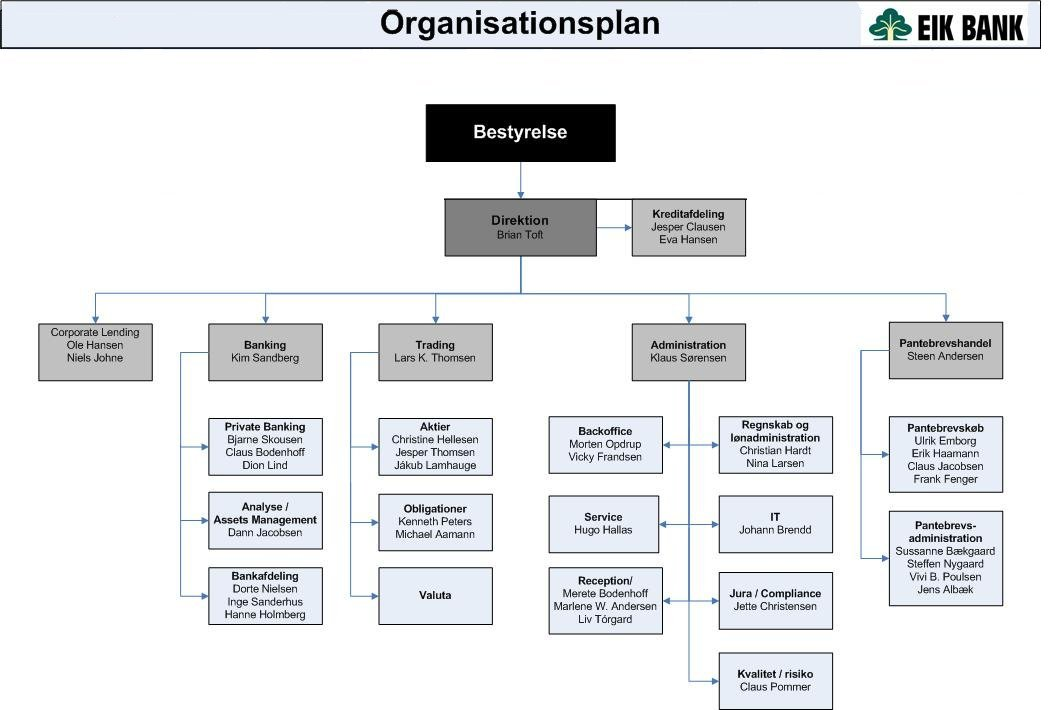
\includegraphics[scale=1.1, width=1.0\textwidth]{Billeder/Organisationsplan.jpg}
	\caption{Organisationsplan}
	\label{Organisationsplan}
\end{figure}
\end{center}




\newpage
\section{Problemstilling}

Det problemomr�de vores projekt ligger inden for, er de private kunder der s�ger r�dgivning af deres formuer, og h�rer dermed ind under Private Banking.

Private Banking best�r af r�dgivning af kunder og planl�gning af deres �konomiske forhold. De �konomiske forhold deles op i indt�gts-, formue- og pensionsforhold. Kunderne kan for eksempel f� r�dgivning om hvordan kundens �konomi ser ud i tilf�lde af uarbejdsdygtighed, hvordan man bedst sikrer sig en optimal udnyttelse af kundens likvider, om disse likvider kan omstruktureres og s� videre. Det prim�re problem best�r i at kunne vise kunderne en trov�rdig oversigt over og simulering af nuv�rende og fremtidige forhold. Man fors�ger at sikre kunden bedst mulige �konomiske vilk�r fremover, ud fra det grundlag kunden st�r med.

Problematikken med afdelingens nuv�rende arbejdsgang drejer sig hovedsageligt om de v�rkt�jer r�dgiverne har til r�dighed. Bankens Private Banking afdeling benytter i dag Excel regneark, hvor alle tal og forhold indtastes, behandles via formler og derefter printes ud til kunden. Et eksempel p� det nuv�rende system kan ses i bilagene, bilag \ref{Eksisterende}, side \pageref{Eksisterende}.
Indtastningen af kundens data sker ud fra det materiale kunden kommer med, som er p� papirform. Dette materiale drejer sig typisk om depotoversigter, selvangivelser, �rsopg�relser med mere. Sammens�tningen af materialet er endvidere forskelligt fra kunde til kunde, hvormed registreringen af oplysningerne ikke kan g�res til en automatiseret process. R�dgiveren skal alts� holde styr p� papirene samtidig med at de relevante data observeres og tastes ind. Derfor er det vigtigt at indtastningsdelen p� sk�rmen er s� nem at have med at g�re som muligt, hvilket man ikke kan sige at regneark er. 
I regneark har man adgang til alle felter, man kan komme til at skrive i det forkerte felt og slette data der ikke skulle v�re slettet. Endvidere skal man selv s�rge for at slette tidligere data fra hvert felt, da den skabelon regnearket kopieres fra er en tidligere sag. 
Afdelingens r�dgivere �nsker sig i dette regi et v�rkt�j der kan lette indtastningen af kundens data. 

Endvidere m� muligheden for at lave pr�sentable udprint, baseret p� regneark, siges at v�re begr�nset. Dette beskrives af afdelingens r�dgiverer som et andet af hovedproblemerne, at \emph{``man er ikke n�dvendigvis stolt af det resulterende materiale man giver til kunden''}.
Problemet er at servere en �konomisk oversigt for kunden, p� en mere overskuelig og pr�sentabel m�de.

Et andet problem best�r i at kundernes data i Private Banking afdelingens system ikke er centraliseret. Sagerne gemmes p� et f�lles netv�rksdrev. Alle har samme adgangsrettighed til denn mappe. Hver r�dgiver holder yderligere styr p� sine kunder i personlige adressekartoteker, da en kunde normalt tilknyttes �n og samme r�dgiver, som f�lger kunden s� l�nge kunden er tilknyttet banken. Dette kan give problemer hvis en r�dgiver bliver syg, og de andre derfor ikke har adgang til disse data.
\section{Form�l med systemet}

Dette afsnit opsummerer hovedpunkterne fra problemstillingen og anskuer form�let med det nye system fra EIK Banks side.

Det overordnede form�l med det nye system er at g�re det nemmere for den private kunde at f� et overblik over sin �konomi, p� en professionel, indbydende og pr�sentabel m�de. Banken er ikke tilfreds med deres nuv�rende v�rkt�j som det prim�re arbejdsredskab og ser dette som et problem.

Yderligere er det et m�l at lette bearbejdningen af data for EIK Banks Private Banking r�dgivere. Det er relativt besv�rligt og usikkert at arbejde med Excel p� indtastnings- og beregningsniveau, hvor en applikation med windows-form brugergr�nseflade tilbyder langt bedre h�ndtering og sikkerhed. Med sikkerhed t�nkes blandt andet p� at man ikke kan komme til at skrive eller slette elementer der ikke er adgang til, som man kan i et regneark.

Det er endvidere et m�l at samle r�dgiverens v�rkt�jer i �n applikation. Disse v�rkt�jer indbefatter de nuv�rende Excelark og dokumenter, fremskrivningsskabeloner, adressekartoteker og tabelopslag p� diverse offentlige instansers hjemmesider.

\newpage




\newpage
\section{Problemformulering}

Ud fra de betragtninger vi har gjort om det eksisterende system, hvor EIK Bank anvender Excel regneark til simulering af private kunders �konomi, ses det tydeligt at et nyt system vil kunne bidrage med v�sentlige forbedringer. Disse forbedringer vil til dels komme r�dgiveren og dennes arbejdsgang til gode og dels vil de komme kunden til gode ved et hurtigere og bedre overblik, i form af et mere professionelt udprint. Systemet skal ikke lave v�sentligt om p� de processer der ligger i den nuv�rende arbejdsgang, men g�re det lettere at udf�re arbejdet. For at vi kan finde ud af hvordan det nye system skal konstrueres, er det n�dvendigt at analysere en r�kke forhold, hvoraf problemformuleringen kan defineres:

%Hvordan kan vi udvikle et bruger- og udvidelsesvenligt system til private banking, som giver kunden et forbedret overblik over deres �konomiske forhold, i forbindelse med registrering af kunders privat�konomi.\\
%Vi vil yderligere unders�ge hvordan vi kan skabe et godt design af brugergr�nsefladen og om vi med fordel kan inddrage elementer fra eksperimentiel systemudvikling i processen. Vi er endvidere interesserede i at implementere systemet ved hj�lp af design patterns, hvorfor vi vil unders�ge hvilke der kan v�re relevante for vores system.

EIK Bank har et krav om at systemet skal v�re brugervenligt, kunne udskrive professionelt udseende rapporter til kunden og skabe gennemskuelighed og overskuelighed af kundens �konomi. Hvordan kan vi opfylde dette krav ved inddragelse af eksperimentielle systemudviklingsmetoder og teori om brugervenlighed?

Et andet krav siger at systemet skal v�re modul�rt og udvidelsesvenligt. Kan vi ved brug af design patterns opfylde dette krav, og i s� fald med hvilke design patterns?



%\begin{itemize}
%\item Hvordan f�r vi skabt et optimalt design af brugergr�nsefladen?

%\item Vi er interesserede i at implementere systemet ved hj�lp at design patterns. Hvilke fordele kan vil f� for systemet? Hvilke design patterns er relevante for denne applikation?

%\item Vi er endvidere interesserede i at inddrage aspekter af eksperimentiel systemudvikling i projektet. Hvordan vil dette p�virke projektforl�bet?

%\item Hvad kan vi g�re for at systemet ikke tilpasses den ene r�dgivers arbejdsform mere end den andens?

%\item Hvordan kan vi forbedre systemets visualiseringsgrad overfor kunden, med hensyn til udprint af data?
%\end{itemize}








\chapter{Metodologi}
\section{Metodologi}

Med henblik p� den grundl�ggende metodologi handler dette afsnit om de filosofier og principper vi har arbejdet efter og hvordan de er blevet anvendt.

For at beskrive en metodologi kigger vi p� hvordan projektet er nedbrudt i faser, hvilke opgaver der skal udf�res i hver fase og hvilket output der skal produceres. Yderligere ses der p� hvem der involveres i faserne og opgaverne, hvorn�r de udf�res og hvordan projektet skal styres. Man kan, hvis man finder det n�dvendigt, ogs� se p� hvilke forhold opgaverne udf�res under og hvilke hj�lpev�rkt�jer man kan tage i brug. Se kilde \cite{ISD}.

I projektets f�rste uge fokuserede vi p� at blive enige om hvilke principper vi ville arbejde efter og have som styrings\-principper.

\subsection{Filosofier}

Vi blev hurtigt enige om f�lgende, helt grundl�ggende, principper eller filosofier om man vil:

\begin{itemize}
\item Vi vil fors�ge at arbejde ud fra en risiko-drevet tankegang, forst�et p� den m�de, at den n�ste opgave vi skal l�se skal v�re den opgave der er st�rst konsekvens ved ikke at f� l�st. Hermed er vi hele tiden opm�rksomme p� ``at kn�kke den h�rdeste n�d f�rst''.
\item Vi har et princip om at vi skal dele rollerne mellem os p� en s�dan m�de at de roterer blandt os. Dette er for at mindske risikoen for at vi sidder fast i gamle rutiner og arbejdsformer. Nogle er for eksempel mere vant til at styre m�der og prototypesessioner end andre og andre er mere vant til at holde sig i baggrunden og observere. Nogle er gode til at kode, hvor andre er bedre til det systemudviklingsm�ssige aspekt. Det skal ikke v�re fastlagt at dem der er vant til en opgave, dermed er selvskrevne til at udf�re opgaven n�ste gang. Vi vil derudover ogs� p� denne m�de hver i s�r fors�ge at udvikle os p� andre omr�der end vores kerneomr�der. Der er dog ogs� et paradoks med denne rotation, p� den ene side skal alle v�re med til alt, p� den anden side kan der spares tid og udvikles mere effektivt, hvis folk laver det de er bedst til. Her kan f�lelsen af tidspres, v�re den faktor der g�r at man afviger fra sit princip.
\item Vi inddrager elementer fra eksperimentiel systemudvikling. Her t�nkes specielt p� prototyping. Vi vil endvidere anvende elementer fra de agile metoder, hvor for eksempel det daglige morgenm�de er inspireret af den agile udviklingsmetode Scrum. De agile metoder er netop kendetegnet ved at v�re fleksible og kunne tilpasse sig forl�bet, ved hyppig opf�lgning p� processen.
\item I forbindelse med kravindsamling vil vi g�re brug at prototyping, som et 'RAD'\footnote{Rapid Application Development} moment. Vi vil prim�rt g�re brug at den papirbaserede Lo-Fi \footnote{Low Fidelity} prototype, kombineret med video- og lydoptagelse af sessionerne.
\item Aktiv brugerdeltagelse er v�sentlig for os, hvorfor vi afholder en ugentlig briefing for de, i projektet, involverede personer fra EIK Bank. Udover dette inddrager vi brugerne i udviklingen, her t�nkes p� prototypesessioner, kravindsamling, m�der med mere.
\item Vi anvender ikke UP\footnote{Unified Process}. Hermed menes, at vi ikke deler vores projektforl�b op i inception, elaboration, construction og transition, i en fastlagt iterativ process. I forbindelse med dokumentation over for opgaven arbejdes der ikke efter en dokumentdrevet tankegang (dette er med inspiration fra XP). Vi har, i opgaven, ikke noget �nske om at lade os drukne i dokumentation. I forhold til selve systemet m� vi dog stille vores eget �nske om let dokumentgang til side og lave den grad af dokumentation som virksomheden �nsker. Vi vil alts� tage elementer fra UP i brug n�r vi f�ler det bliver relevant.
\item Vi vil, og skal, stille s� mange ``dumme'' sp�rgsm�l som muligt. Ikke for at stille dumme sp�rgsm�l, men for at f� de bedst mulige forklaringer p� de ting vi sp�rger om. Problemet er at vi, s�vel som de involverede medarbejdere fra EIK Bank, er fagspecialister p� hver vores omr�de. Derfor kan det v�re vanskelig at kommunikere med hinanden p� en s�dan m�de at alle parter forst�r hinanden. Derfor vil vi hellere sp�rge ind til et problem en gang for meget, end en gang for lidt.
\end{itemize}

\subsection{Arbejdsform}
Det overordnede framework for projektet er inspireret af spiralmodellen og dens iterative adf�rd. Vi nedbryder dermed projektforl�bet i faser. Herunder er det fastlagt, at vi har korte iterationer p� 1 uges varighed.
\begin{itemize}
\item For hver iteration skal der l�ses fastlagte opgaver:
\begin{itemize}
\item Dagen starter med at afholde et internt morgenm�de, hvor der bliver gjort status og lavet dagsorden for hvad der skal laves den p�g�ldende dag, se Bilag \ref{Morgenmoeder} p� side \pageref{Morgenmoeder}. Dette er efter forbillede af XP og Scrum. Dagsordenen nedskrives til hvert m�de og gemmes.
\item N�r dagen er omme skrives der dagbog, hvor der bliver noteret hvad der er lavet og sket, se Bilag \ref{Dagboeger}.
\item Der laves en ugentlig planl�gning af n�ste iteration. Dette vil sige at der hver fredag bliver lavet en plan for n�ste uges forl�b og denne uges m�l. Det ugentlig m�l resulterer typisk i f�rdigg�relsen af et eller flere af projektets delm�l, alts� et delsystem. Hver iteration l�ber fra fredag til torsdag, hvormed deadlinen for ugens m�l er fredag morgen. Den ugentlige plan nedskrives og gemmes. I dette planl�gningsforl�b opklares hvad der i kommende iteration er den ``h�rdeste n�d''. Dette g�res internt i gruppen.
\item Der afholdes et ugentligt informationsm�de med vores kontaktpersoner fra EIK Bank. Dette er for at vise fremskridt, engagement, �benhed og for at bevare interessen omkring vores arbejde. Endvidere er vi interessede i l�bende at sikre os at vi og EIK Bank er enige om det arbejde der bliver udf�rt. Efter m�derne skrives der referater, som vi bruger til at behandle indtryk fra og resultater af m�derne. M�det er stilet mod vores to kontaktpersoner fra private banken afdelingen, samt to medarbejdere fra IT-afdelingen. 
\item Der skal bruges tid p� at skrive rapport mindst �n gang om ugen. Som udgangspunkt sker dette hver fredag, hvormed fredag bliver en ``skrive-dag''.
\end{itemize}
\end{itemize}

\subsection{Vore erfaringer med v�rkt�jer og metodologien}

Noget af det f�rste vi erfarede i forbindelse med vores principper, var at m�l og planer ikke har nogen effekt hvis der ikke er konsekvens bag ordene. Det er ikke hensigtsm�ssigt bare at rykke en deadline eller lade v�re med at opfylde et m�l, hvilket kan ske hvis der ikke er nogen konsekvens ved at g�re det. Dermed er det vigtigt at f� defineret sine m�l pr�cist og at m�lene holdes inden for s� realistiske rammer som muligt. Ved at v�re opm�rksom p� dette f�r vi ogs� bedre mulighed for at f� success med at planl�gge os ud af eventuelle problemer. 

Et af de f�rste m�l, der kunne opfattes som en h�rd n�d, var at bestemme hvilken database der skulle anvendes og hvor denne database skulle ligge. L�s mere om denne problematik i \ref{Database}, p� side \pageref{Database}. For at f� svar p� dette sp�rgsm�l skrev vi en mail, der blev sendt videre til bankens datacentral. Problemet var dog at vi ikke havde talt om hvad vi skulle g�re hvis vi ikke fik svar p� mailen inden vores deadline udl�b. Dette fik vi ikke og dermed stod vi med et problem. Efter en del overvejelser blev det vedtaget at holde os til planen, i henhold til ovenst�ende afsnit. Dette gjorde vi ved at tage en beslutnig om at arbejde videre med en l�sning som vi vidste var mulig, nemlig at anvende en Access database, fremfor at risikere at spilde tid p� en uholdbar l�sning. Vores tanker og �nske om at arbejde med en mere avanceret databasel�sning blev dermed droppet og vi havde nu n�et vores m�l.

De daglige rutiner, her t�nkes specielt p� morgenm�det, har vist sig at have en god effekt p� arbejdsgangen, p� flere m�der. For det f�rste hj�lper morgenm�det til at sikre at alle gruppemedlemmer ved hvad der er lavet, hvad der skal laves, hvad der foreg�r og hvem der laver hvad. M�det er yderligere en god m�de at sikre at der bliver taget h�nd om vigtigste problemer, i henhold til ugeplanl�gningen. Det er alts� et et godt v�rkt�j til at holde fokus p� det arbejde der skal udf�res og til at holde styr p� hvad der er lavet. Her er dagbogen ogs� et hj�lpev�rkt�j som vi, i samspil med morgenm�det, har haft gavn af. Dagbogen er knapt s� formel og kr�ver ikke n�dvendigvis et decideret m�de internt i gruppen, men gemmes og giver mulighed for tilbageblik og status, se Bilag side \pageref{Dagboeger}.

Den ugentlige planl�gning af n�ste iteration har v�ret en effektiv m�de til at identificere de mest presserende problemer og til at koordinere den tid der har v�ret til r�dighed. Med denne planl�gning har vi, som f�r skrevet, haft fokus p� at identificere de ``h�rdeste n�dder''. De sidste to uger af projektet, har vi dog ikke haft overordnede m�l for udviklingen, da ugerne har v�ret reserveret til rapportskrivning. Rapportskrivning mener vi umiddelbart ikke kan planl�gges og koordineres s� lang tid i forvejen, hvorfor der ikke udf�rt ugeplanl�gning i denne fase.

Iterationens l�ngde og varighed, fra fredag til og med torsdag, har v�ret et punkt der tog noget l�ngere tid at beslutte sig for. Et argument mod den valgte varighed, har v�ret at vi reelt kun har haft 4 dage til udviklingen i hver iteration, i og med at fredag, som iterationens f�rste dag, hovedsageligt er blevet brugt til fredagsbriefing, planl�gning af iterationen samt rapportskrivning. Man skal dog huske p� at disse ting ogs� er vigtige at tage sig tid til. Vi har alts� haft mulighed for, via fredagens aktiviteter, at planl�gge, koordinere og vurdere hvilke m�l der skal s�ttes for iterationen. Dette har virket ganske godt og vi f�ler selv at have sat relativt realistiske m�l.

For at ``holde kontakten'' med virkomheden og dens medarbejdere har vi, som skrevet, afholdt et briefingsm�de hver fredag kl 09:30. Vores agenda, til dette m�de, har v�ret at forklare hvad vi har lavet i den forgangne uge og hvad planen er for den kommende uge. Der er blevet forberedt en invitation til hvert m�de, hvor dagsordenen er blevet pr�senteret p� punktform. Denne invitation er blevet sendt ud til de relevante personer dagen inden. Dette har vi til dels gjort for at give medarbejderne en mulighed for at bed�mme om m�det kunne v�re interessant for dem eller ej og dels for at give medarbejderne mulighed for at forberede sig til m�det.
Vi f�ler at vi har opn�et en god kontakt med bankens medarbejdere via briefingsm�derne og vi har uden tvivl f�et sat mange ting p� plads og im�dekommet tvivl og misforst�elser. For eksempel havde vi p� et tidspunkt taget en afgr�nsningsm�ssig beslutning, hvor vi var af den opfattelse at fremskrivningerne var vigtigere end udprintsfunktionaliteten. Dette fremlagde vi til m�det og det viste sig at EIK Bank ikke var enige i denne prioritering. Hermed undgik vi at arbejde videre ud af ``et forkert spor'' og vi valgte, som resultat af m�det, at lytte til EIK Banks mening og fokusere p� udprintningen.

Et af de f�rste projektstyringsm�ssige tiltag vi tog, var at udvikle en tidslinie over projektforl�bet p� kalenderform. Denne tidsplan fylder �n A4 side og er inddelt i 10 uger, fra d. 30. januar til d. 3. april. Det gav os et tidligt overblik over hvor mange iterationer vi har haft til r�dighed og hvordan tiden kunne prioriteres. Ud fra dette overblik blev vi enige om f�lgende inddeling:

\begin{itemize}
\item Uge 4: Den f�rste uge af projektet g�r med planl�gning, indledende tanker og installation p� kontoret.
\item Uge 5, 6, 7, 8, 9, 10 og 11: De 7 uger/iterationer vi har til analyse, design og implementering.
\item Uge 12 og 13: Rapportskrivning.
\end{itemize}

I forbindelse med den mere praktiske del af projektstyringen, har vi fra starten anvendt et system til versionsstyring. Systemet hedder SVN\footnote{Subversion} og tager sig af h�ndtering af dokumenter, kode og andet, med andre ord alt vores materiale. Systemet fungerer som en server- og klient l�sning, hvor serveren holder og styrer repositoriet hvor data ligger. Denne Subversion serverapplikation k�rer p� en ekstern Linux server. Via Windows-klienten Tortoise SVN kan man tilf�je nyt materiale, redigere i det eksisterende materiale og hvis noget skulle g� galt, genskabe data fra tidligere revisioner. Vi har haft adgang til projektets data derhjemme, n�jagtig som vi har haft det p� vores computere p� EIK Bank. Systemet holder styr p� hvem der har lavet hvad og hvorn�r det er blevet lavet. Data slettes aldrig fra repositoriet selvom det bliver slettet via klienten, det bliver bare fjernet fra den aktive del af repositoriet, hvorfor man altid har mulighed for at finde data frem igen.

%==
%
%Er vi p� vej over i at identificere n�dder i kraft af, at der er ting vi ikke har erfaring med. Jeg (klaus) mener ikke at manglende erfaring g�r en n�d til en h�rd n�d. Det er ogs� meget vigtigt er der er enighed i gruppen om hvad der er den h�rdeste n�d. En anden type n�d kunne ogs� v�re af kommunikations-/forst�elsesm�ssig karater.

%Vi har haft et lille problem med kommunikationen med kunden. Vi har kommet til at give udtryk for at det ikke er noget problem at lave det Ene og det andet p� det nye system. Det er i sig selv ikke noget problem, men dette kan komme til at fremst� som et l�ft for hvad det nye system kommer til at indehode. Det er meget vigtigt at vi i samarbejde med kunde er enige om hvad der er �nskeligt og hvad der er muligt. Specielt set i lyset af den meget begr�nsede tid vi har til vores r�dighed.

%Holde flere og samtidigt kortere sessioner, hvormed kvaliteten gerne skulle blive bedre. Afgr�ns sessionerne bedre.


\chapter{Kravindsamling}
\section{Prototyping}

\subsection{Vores brug af prototyping}
For at skabe en, mellem udvikler og bruger, f�lles forst�else af systemet, kan det v�re ganske frugtbart og forholdsvist omkostningsfrit at bygge en prototype og bruge denne som en pr�-udviklingsplatform. Der findes forskellige former for prototyper, som har det til f�lles at de er meget dynamiske og relativt lette samt omkostningsfrie at lave �ndringer i. Hermed er det ikke altafg�rende at prototypen er komplet, fra f�rste gang den anvendes i en session mellem udviklere og brugere. Det vigtige er, at man kommer hurtigt i gang med at specificere krav, snakke layout, unders�ge workflow med mere. Prototyping er alts� et eksperimenterende element i vores systemudviklingsmetode, som st�r i kontrast til den typisk mere dokument- og analysedrevne og 
traditionelle form for systemudvikling, s�som Unified Process.

Det vigtigste aspekt i forbindelse med prototyping er fasts�ttelsen af krav til systemet. I denne henseende er prototyping lige s� meget et hj�lpev�rkt�j for kunden/brugeren, som for udviklerne, da kunden langt fra altid selv er klar over hvilke krav de har til et fremtidigt system. Kunden f�r et tidligt indblik i systemet og dermed l�ngere tid til at t�nke over hvad de vil have systemet til at kunne. 

Netop aspektet med at man hurtigt kommer igang med at visualisere systemet og fastl�gge krav, ligger til grund for vores valg af prototyping-teknik, nemlig Lo-Fi. prototyping teknikken. Lo-Fi er en papirbaseret prototype der repr�senterer et sk�rmbillede af det fremtidige system. Under sessionen uddeles der roller til udviklerne, nemlig facilitator, 'computer' og observat�r. Det er udviklernes opgave at afholde og styre sessionen, hvor kunden/brugeren bliver pr�senteret for prototypen og en r�kke scenarier der skal gennemg�s. Kunden/brugeren kan nu udf�re den stillede opgave ved at 'lege' at han anvender systemet, hvor 
'computeren' s�rger for at systemet udf�rer det kunden/brugeren g�r. Vi har endvidere valgt at anvende Midi-Fi\footnote{Midi-Fidelity.} prototyping, i form af video-, billeder og lydoptagelser af vores prototype sessioner, til dels for at st�tte observat�ren og til dels for at dokumentere vores process, se figur \ref{prototype2_KundeData} p� side \pageref{prototype2_KundeData}, figur \ref{prototype2_FormueForhold_popup1} p� side \pageref{prototype2_FormueForhold_popup1} og figur \ref{prototype2_FormueForhold_popup2} p� side \pageref{prototype2_FormueForhold_popup2}.

Prototyping er, som f�r n�vnt, et eksperimenterende v�rkt�j, hvorfor det er vigtigt for udviklerne at have en god forst�else for og et godt kendskab til prototyping. Der er mange situationer hvor manglende styring og mangelfuld forberedelse v�sentligt kan mindske det udbytte man f�r af en prototype. Ved at unders�ge teorien omkring prototyping, inden man anvender teknikken, opn�r man det bedste resultat. Vi har som studerende p� datamatiker\-uddannelsen haft prototyping og eksperimentiel systemudvikling som emne p� fjerde semester, hvor vi udover at studere teorien, lavede prototyping studiegrupperne imellem. Det er ud fra denne erfaring at vi har anvendt prototyping i forbindelse med vores hovedopgave projekt hos EIK Bank.

Som udgangspunkt har vi lagt fokus p� indtastningsdelen af systemet og har derfor udviklet  prototyper til denne. Vi har startet med at l�gge fokus p� indtastingsdelen, da denne del er vital for resten af systemet. Den var det mest logiske sted at begynde, da ingen af systemets resterende delsystemer, fremskrivninger og udprintning, kan eksistere uden en fungerende indtastningsdel. Yderligere udtrykte EIK Bank �nske om et mere afgr�nset og velfungerende produkt, hvorfor vi ikke �nskede at gabe over for stor en mundfuld.

Til at simulere de opgaver en bruger kan komme ud for, har vi f�et materiale i form af en rigtig sag fra private banking. Ud fra dette materiale kunne vi derfor skabe trov�rdige scenarier.

\subsection{Prototype 1}

Vi har arbejdet med denne prototype i projektets anden uge/iteration.

\subsubsection{Form�l}
\begin{itemize}
\item At f� et tidligt indblik i EIK Banks arbejdsgange i forbindelse med indtastning af en kundens stamdata 
og �konomiske forhold.
\item At f� afpr�vet vores visioner omkring systemets virkem�de.
\item At f� indsamlet krav og specificeret krav til systemet.
\item At f� �velse i at afholde prototyping-sessioner.
\end{itemize}

\subsubsection{Setup}

Vi valgte at bygge vores f�rste prototype p� basis af en, i gruppen, intern brainstorming. Her brugte hvert medlem af gruppen en halv time p� at forme sin egen version af systemet. Ud fra de resulterende skitser evaluerede vi vores ideer og tanker og samlede derfra det bedste fra hver udgave, til et samlet udkast. Dermed blev prototype 1 til. Se vedlagte billede under bilag, reference. 

Der blev afholdt en session med vores kontaktpersoner fra private bank\-ing, som begge er r�dgivere, hvor setup'et var ens i form af samme prototype og scenarier. Grunden til at vi holder en session med hver r�dgiver er, at vi gerne vil have den enkelte r�dgivers personlige mening og opfattelse. Vi var ikke interesserede i at r�dgiverne kommer til at farve hinandens udmeldinger eller p� anden m�de p�virker hinanden. Vi anvendte videooptagelse af sessionerne, for at fastholde dokumentationen. Gruppemedlemmerne var tildelt roller, i form af facilitator, 'computer' og observat�r. Til sessionerne forberedte vi scenarier til brugeren, som havde til form�l at simulere situationer brugeren kan komme ud for i den nuv�rende arbejdsgang. Den f�rste session var planlagt til at vare 1 time, hvor brugeren skulle gennemg� de opstillede scenarier, nemlig 4 styk:

\begin{enumerate}
\item \emph{Indtast kundens stamdata ud fra det udleverede materiale.}
\item \emph{Indtast kundens indt�gtsforhold.}
\item \emph{Indtast kundens formueforhold.}
\item \emph{Indtast kundens pensionsforhold.}
\end{enumerate}

\subsubsection{Gennemf�relse}
	
\subsubsection{Session 1}

Vi startede med at pr�sentere os selv og vores roller. Derefter forklarede vi hvad vi havde planlagt til sessionen og hvad vi gerne ville n� frem til. Derudover spurgte vi om det var i orden at vi optog forl�bet p� video, dette fik vi en accept af. Sessionen blev gennemf�rt ved gennemgang af scenarierne, dog tog den l�ngere tid end planlagt, vi overskred tidsplanen med cirka et kvarter.
Der blev afrundet med evaluerende sp�rgsm�l og indtryk fra b�de os og r�dgiveren.

\subsubsection{Session 2}

Denne session var, som session 1, planlagt til at vare 1 time. Vi ville her fors�ge at v�re bedre til at overholde tidsplanen. Vi fors�gte at bruge lidt mere tid p� at introducere og forklare forl�bet, opdelingen af vores roller under sessionen og hvad det i det hele taget gik ud p�. Vi fik igen accept af brugen til at video\-optage. Scenarierne blev gennemg�et, men det lykkedes desv�rre ikke at holde sessionen indenfor den planlagte tidsramme. Sessionen blev afsluttet med en evaluering af forl�bet.

\subsubsection{Samlet evaluering}

Vi fandt ud af hvor vigtigt det er at tage sig tid til at f� forklaret hvad form�let med en session er, hvad den indeb�rer, hvad rollerne indeb�rer og hvordan brugeren kan interagere med systemet. For eksempel burde vi have brugt flere kr�fter p� at forklare, at 'computeren' udelukkende reagerer p� sessionsdeltagerens input og ikke g�r andet end det. Dette punkt m� gerne g� lidt langsomt. Vi var ikke alt for gode til dette, hvilket er en erfaring vi vil tage med os til n�ste session. 

Vores brugere er r�dgivere af natur. Hermed menes at de er vant til at styre samtaler og dialog. Dette menes ikke som en kritik, men som en konstatering af at facilitator skal v�re ekstra opm�rksom p� at styre sessionen, hvilket vi oplevede var sv�rt. 'Computeren' var generelt ikke opm�rksom p� at melde fejl n�r brugeren udf�rte noget ulovligt, hvilket skaber forvirring i situationen. Denne forvirring udmynter sig i misforst�elser af hvad systemet kan og man risikerer at brugeren tager styringen. Det er en �velse at overholde de roller man har, hvilket ikke altid lykkedes lige godt selvom vi havde planlagt dem godt. Da vi har et princip om job-rotation, skiftede rollerne fra session 1 til session 2. Dette betyder ogs�, at man ikke kan specialisere sig s� meget i en rolle, og dermed m� forvente at det tager l�ngere tid f�r samarbejdet kommer til at k�re som �nsket. 

Gennem evaluering af vore egne indsatser, har vi fors�gt at blive bedre til at overholde og respektere de roller der er tildelt. Det er for eksempel ikke hensigtsm�ssigt, som computer, at afbryde facilitator midt i en instruktion. Yderligere er det at l�re og forst� hvordan folk hver is�r arbejder, og er forskellige, et punkt vi har arbejdet med. 

Det kan v�re en stor hj�lp for brugeren at lave et forklaringsark, hvor symbolerne (knapper, radioknapper, tekstfelter, osv.) p� prototypen er beskrevet. Dette forklaringsark skal ligge fremme, til adgang for brugeren. Hermed har brugeren hele tiden muligheden for at bevare overblikket og ikke standse for meget op hvis han bliver i tvivl om hvad symbolerne betyder. Vi havde ikke et s�dan forklaringsark under session 1, hvor vi observerede at brugeren enten havde glemt betydningen af eller ikke forstod symbolerne. Dette fik vi fulgt op p� under session 2, med godt resultat. 

Det er vigtigt at de sk�rmbilleder der ikke bruges gemmes for brugeren. Hvis ikke dette g�res risikerer brugeren at blive distraheret og springe i sk�rmbillederne, uden at bede computeren om det, hvilket mindsker graden af en realistisk simulering af en computers virkem�de. Yderligere forstyrrer det den plan vi har lagt for forl�bet. P� den anden side gav det os en forst�else af, at en stor grad af fleksibilitet i systemet er n�dvendig. Samtidigt fandt vi ud af at den navigeringsbar mellem sk�rmbillederne som vi havde lavet, mindskede graden af fleksibilitet da den var l�st. Hermed menes at navigeringen foregik �t sk�rmbillede af gangen, uden mulighed for at springe et sk�rmbillede over. Dette p�pegede r�dgiveren i session 2 som et problem. 

Generelt fik vi rigtig meget god information ud af sessionerne med prototype 1. Vi blev meget klogere p� systemet og de nuv�rende arbejdsgange.

Vi vil gerne blive bedre til at estimere og forudsige varigheden af de sessioner vi afholder. Noget af det vi har gjort for at estimere er at vi hver is�r er kommet med vores bud p� hvor lang tid en session vil tage og derefter ligge lidt til, for at fors�ge p� at v�re p� den sikre side. Det har dog desv�rre, hver gang, vist sig at vi har lagt for lidt tid til. Vi fik god �velse i prototyping og mange erfaringer med p� vejen.

\subsection{Prototype 2}

Vi har arbejdet med prototype 2 i projektets tredie uge/iteration.

\subsubsection{Form�l}
For at sikre kvalitet og for at f� et optimalt udgangspunkt for at g� i gang med design\-fasen, har vi valgt at udvikle en forbedret version af prototypen, en 'f�rdig' prototype, om man vil. Denne prototype har de foresl�ede forbedringer fra prototype 1 med, samt at vi valgte at l�gge en del mere v�gt p� layout og udformning. Form�let med disse forbedringer var at g�re det nemmere at f� indholdet til at v�re der p� en p�nere og mere pr�sentabel m�de. 

Til denne session har vi �nsket en samlet gennemgang, diskussion og dialog omkring forbedringer og eventuelle forv�rringer, og undladt at basere sessionen p� scenarier. Diskussionen �nskede vi skulle foreg� mellem r�dgiverne, vi gav dog ikke udtryk for dette, da det helst skulle komme af sig selv. Hermed �nskede vi at f� dem til at stille hinanden sp�rgsm�l, som vi ikke selv ville kunne have t�nkt p�. Faremomentet er at de som fagfolk kan komme til at tale s� specifikt at vi som udenforst�ende ikke kan forst� pointerne.

M�let med denne prototype kan opfattes som et kvalitetscheck af de allerede indsamlede data og en 
konfirmation af hvad vi er blevet enige om med kunden.

Form�let er alts� at pr�cisere hvilke felter der skal v�re i indtastningsdelen i systemet.

\subsubsection{Setup}
Til prototypen brugte vi forskelligt farvet papir til at skelne mellem elementer, og sk�rmbilledearealet var dobbel s� stort. Til denne prototype blev der afholdt en samlet session med de to medarbejdere der deltog i sessionerne med prototype 1. Hvor vi i forbindelse med prototype 1 valgte at dokumentere p� video\-form, valgte vi i forbindelse med prototype 2 at n�jes med at optage lyd. Grunden til dette var at det var mere praktisk at n�jes med lydoptagelse p� grund af det udstyr vi havde til r�dighed, som ikke kunne optage video i mere end 3 minutter af gangen. Ved at lave lydoptagelse var vi fri for besv�ret med hele tiden at skulle tjekke udstyret. Derudover f�lte vi at det ikke var n�dvendigt at dokumentere endnu en session med video, da det tager l�ngere tid at behandle og bearbejde. Derudover tog vi et almindeligt foto af hver sk�rm i prototypen, for hver gang et sk�rmbillede blev debateret f�rdig og der blev enighed om hvad sk�rmbilledet skulle indeholde. Dette foto brugte vi som dokumentation af de forskellige sk�rmbilleders indhold. Der var igen tildelt roller til gruppemedlemmerne og der var afsat 1 time til denne session, se figur \ref{prototype2_KundeData} p� side \pageref{prototype2_KundeData}, figur \ref{prototype2_FormueForhold_popup1} p� side \pageref{prototype2_FormueForhold_popup1} og figur \ref{prototype2_FormueForhold_popup2} p� side \pageref{prototype2_FormueForhold_popup2}.

\subsubsection{Gennemf�relse}
Vi startede med at pr�sentere de 2 brugere for hvad form�let med sessionen var og informerede om hvordan forl�bet var planlagt. Vi forklarede at der var afsat 1 time til sessionen. Vi fik som svar hertil igen at vide at det tager den tid det tager og at vi ikke n�dvendigvis skal stoppe f�r sessionen er fuldendt. Herefter blev der startet fra f�rste sk�rmbillede og frem, hvor hvert sk�rmbillede blev gennemg�et og vurderet. Yderligere blev de enkelte situationer, hvor indholdet af sk�rmbilledet �ndrer sig, alt efter hvad man trykker p�, vurderet. Hver f�rdig sk�rm blev, som planlagt, fotograferet.

\subsubsection{Evaluering}
Selvom sessionen desv�rre tog dobbelt s� lang tid som planlagt, f�ler vi at den forl�b godt. Den forl�b velstruktureret, omend det kneb med koncentrationen til sidst p� grund af det lange tidsforl�b p� 2 timer. Som erfaring har vi gjort os at 2 timer er for lang tid, der skal som det mindste v�re en god pause. Det er mere optimalt med 1 times varighed. Vi fik en rigtig god snak om arbejdsgangene og en konfirmation af hvad vi var kommet frem til op til dette punkt. Vi fik udarbejdet en udspecificeret 'f�rdig' prototype, som vi kan opfatte som en 'f�rdig' liste 
over hvad der skal v�re hvor i indtastningsdelen af systemet. Med hensyn til fordelingen af roller og det at overholde disse roller var sessionen rigtig god. Det virkede godt at vi n�jedes med at optage lyd denne gang. Dette aspekt virkede ogs� mere afslappende og uformelt p� brugerne, idet der ikke stod et kamera og filmede hver bev�gelse. Under denne session var vi blevet bedre til at styre sessionen, brugerne og forl�bet. Vi var mere opm�rksomme p� at styringen ikke m� blive delt mellem brugere og udviklere. Vi fik ogs� ros for at tage styringen.

\subsection{Konklusion af vores brug af prototyping}

Vi har fundet ud af hvor vigtigt det er at holde en stram styring af sessionerne og overholde de aftalte roller. 'Computeren' skal ikke g�re andet end at udf�re det brugeren beder den om og melde fejl hvis det er n�dvendigt. Det er facilitators opgave at s�rge for at styre sessionen og brugeren, uden af give for meget hj�lp. Brugeren m� ikke f� lov til at overtage styringen. Ligeledes er det vigtigt at lave en grundig introduktion til sessionen, hvor man tager sig tid til at forklare m�let med sessionen, reglerne for sessionen med mere og hvor man sikrer sig at brugeren har forst�et disse punkter. 

Vi har b�de f�et god prototype-teknisk erfaring og vi har n�et m�let med at f� et tidligt indblik i arbejdsgange og krav.

Vi har fundet ud af at det er sv�rere end som s� at sp� om hvor lang tid en session vil komme til at tage. Sessionerne med prototype 1 tog begge v�sentligt l�ngere tid end beregnet, hvor sessionen med prototype 2 tog dobbelt s� lang tid som planlagt. Dette er selvf�lgelig ikke helt optimalt, b�de planl�gningsm�ssigt for os, s�vel som for EIK Banks medarbejdere. Vi har dog v�ret s� priviligerede at EIK Banks medarbejdere har givet os den tid det m�tte tage at gennemf�re sessioner og m�der, hvormed det i vores situation ikke har v�ret et voldsomt problem at overskride tiden.

\subsection{Konklusion i forhold til systemet}

Vi fik opklaret en masse specifikke sp�rgsm�l omkring hvilke felter, knapper, informationer med mere medarbejderne forventede i hvilke situationer. I denne henseende fandt vi ud af at mindre og smarte features, som for eksempel direkte links til www.skat.dk, skal prioriteres lavere end  kernekravene og den basale funktionalitet i programmet, se afsnit \ref{Kravliste} side \pageref{Kravliste}.

Vi fandt ud af at der er stor forskel p� hvordan medarbejderen griber det udleverede materiale an. En af medarbejderne sorterer f�rst papirerne og deler materialet op efter person, hvor den anden tager papirene �n for �n og stort set i den r�kkef�lge de ligger i. Dette har betydning for os, i og med at systemet skal v�re s� fleksibelt at det kan bruges af, og passer til, alle r�dgiverne. Ydermere er der forskel p� hvordan mennesker interagerer med computere. En medarbejder gik fint i sp�nd med vores r�kkef�lge af sk�rmbilleder, en anden ville gerne have mulighed for at springe i r�kkef�lgen. Dette var endnu et argument for at systemet skal v�re fleksibelt og ikke tilpasset en bestemt type bruger.

Vi fik et mere detaljeret indblik i workflowet, b�de i form af nuv�rende og fremtidige arbejdsgange. Dette er et meget vigtigt punkt, da vores system i f�rste omgang ikke skal �ndre p� private banking afdelingens nuv�rende arbejdsgange, men prim�rt fremme visualiteten og lette behandlingen af data. Dermed er det os der skal konstruere et system der passer til de eksisterende arbejdsgange. Det virkede som om at brugerne, under sessionerne, fors�gte at gennemtvinge deres vante arbejdsgange i det nye system. Dette viser os at det kan v�re vanskeligt og m�ske endda urealistisk, at realisere nye arbejdsgange ved at indf�re en nyt computersystem.

\newpage
\section{Kravliste}

Vi ser det fremtidige system som best�ende af to delsystemer. Et delsystem til indtastning og et delsystem til rapportering. 
\\
\\
\begin{tabular}{ll}
Skala: &1. prioritet betegnes som ``Must have''\\
       &2. prioritet betegnes som ``Could have''\\
       &3. prioritet betegnes som ``Nice to have''\\
\end{tabular}
\\
\\
Til indtastningsdelen har vi fundet f�lgende krav:\\

\tablefirsthead{
  \hline
  \multicolumn{1}{|l|}{Nr} & 
  \multicolumn{1}{p{4.0cm}|}{Krav} & 
  \multicolumn{1}{l|}{Prioritet} &
  \multicolumn{1}{p{5.0cm}|}{Note} \\
  \hline
}

\tablehead{
  \hline
  \multicolumn{1}{|l|}{Nr} & 
  \multicolumn{1}{p{4.0cm}|}{Krav} & 
  \multicolumn{1}{l|}{Prioritet} &
  \multicolumn{1}{p{5.0cm}|}{Note} \\
  \hline
}

\tabletail{
  \hline
  \multicolumn{4}{|r|}{\small Fors�tter p� n�ste side.}\\
  \hline
}
\tablelasttail{\hline}
\bottomcaption{Kravliste.\label{Kravliste}}

\begin{supertabular}{|l|p{4.0cm}|l|p{5.0cm}|}
1  & Systemet skal kunne printe (oversigter, grafer ol.) & 1 & I f�rste omgang 'begr�nset'.\\ \hline
2  & Systemet og udprint skal have et professionelt look & 1 & Genbrug af officiel font, farver, logo, design stil osv.\\ \hline
3  & Kunden ser m�ske programmet under indtastning og skal derfor kunne genkende applikationens stil p� udprintet. 	& 1 & \\ \hline
4  & Rapporten skal udstr�le konservatisme, gennem overskulighed, gennemskuelighed og trov�rdighed. & 1 & \\ \hline
5  & Der skal ikke printes logo.				& 1 & Der bruges brevpapir.\\ \hline
6  & Man skal kunne skifte database ved kun at modificere \'et modul.	& 1 & \\ \hline
7  & Systemet skal kunne bruges af en person som er ind�vet i Private Bankings papirgange, og som kan l�se og skrive. & 1 & \\ \hline
8  & Man skal kunne springe mellem de forskellige indtastningssk�rme.	& 1 & \\ \hline
9  & Systemet skal ikke kr�ve at alle felter udfyldes.		& 1 & Hvis en kunde ikke har nogle pensioner, s� skal disse ikke tastes ind. = fleksibilitet.\\ \hline
10 & Der skal v�re kontrol af typen der bliver indtastet i enkelte felter.	& 1 & Telefon, Cpr m� kun indeholde tal, og s� skal der kun kunne indtastes tal.\\ \hline
11 & Systemet tager sig af positive og negative tal. & 1 & Udgift = negativ, indt�gt = positiv som default. Dette kan �ndres ved at skrive minus foran.\\ \hline
12 & Sk�rmene skal opdatere sig n�r noget nyt er tastet ind.		& 1 & \\ \hline
13 & Der skal v�re labels til indtastningsfelter som siger hvad der skal tastes ind.	& 1 & \\ \hline
14 & Man skal kunne oprette s� mange emner i en kategori p� en gang som muligt.	& 1 & Eksempelvis skal muligheden for at taste renteindt�gt, l�nindkomst osv. ind p� en indt�gtsform v�re til stede uden at formen �bnes og lukkes efter hver indtastning. Med hensyn til aktier og obligationer har man tit mange af og disse skal derfor tastes ind i en datagrid.\\ \hline
15 & Emner der falder uden for kategori skal kunne tastes i et 'Andet' felt.	& 1 & \\ \hline
16 & Rapporten skal have s� f� sider som muligt. & 1 & Set i forhold til at alt skal kunne skrives ud og at det skal v�re overskueligt.\\ \hline
17 & Systemet skal v�re brugervenligt.			& 1 & \\ \hline
18 & Opret, slet, l�s og rediger en session.          			& 1 & \\ \hline
19 & Opret, slet, l�s og rediger en kunde.            			& 1 & \\ \hline
20 & Opret, slet, l�s og rediger et indtaegtsforhold.			& 1 & \\ \hline
21 & Opret, slet, l�s og rediger et pensionsforhold. 		& 2 & \\ \hline
22 & Opret, slet, l�s og rediger et formueforhold.			& 2 & \\ \hline
23 & S�ge p� kunder.				& 2 & \\ \hline
24 & Systemet skal v�re nemt at l�re.			& 2 & \\ \hline
25 & De forskellige lister af Aktiver, Passiver og Pensioner skal have kolonner med summer. En total og en for hver part i familien. 											 & 2 & Er �ndret fra 1 til 2, da det ikke er et prim�rt krav.\\ \hline
26 & Der skal v�re et simpelt notesystem. Dvs. en note der f�lger hele sagen.         				 & 2 & Det har vist sig, pr. 24-02-06, at v�re en 2. \\ \hline
27 & Alle indtastninger skal v�re brutto (alts� f�r skat)                             	    	 & 2 & �ndret fra 1 til 2 da det ikke har det prim�rere fokusomr�de.\\ \hline
28 & Under indt�gtsforhold b�r vi benytte F�R arbejdsmarkedsbidrag.                   	    	 & 2 & �ndret fra 1 til 2 da det ikke har det prim�rere fokusomr�de.\\ \hline
29 & Efter 5-10 sager skal det tage den erfarne konsulent 15-30 min. at taste en kunde ind.    & 2 & Det tager i dag 30-60 min.\\ \hline
30 & Efter 5-10 sager skal det tage den nye konsulent 30-45 min. at taste en kundes data ind.  & 2 & \\ \hline 
31 & Kontrol af indtastninger i felter.   		           		& 3 & Dette kunne v�re modulus 11 kontrol af CPR nr. Det kunne v�re at huske p� at der er renteudgifter forbundet med et l�n.\\ \hline
32 & Der skal v�re et udvidet notesystem. Dvs. noter til hver post i en sag.        					 & 3 & \\ \hline
33 & R�dgiveren skal kunne anvende systemet uden for kontoret.        			                   & 3 & Det har vist sig, pr. 24-02-06, at v�re en 3'er.\\ \hline
34 & Systemet skal kunne simulere fremskrivninger           & 3 & Det har vist sig, pr. 24-02-06, at v�re en 3'er. Auto udregning. Dette afgr�nser vi os helt fra.\\ \hline
35 & Det skal v�re muligt at f� et overblik over kunden og dennes personlige forhold, alts� om kunden er selvst�ndig, bor i udlandet og s� videre.         & 3 & \\ \hline
36 & B�rn: Har de b�rn, hvor mange, deres navne, CPR numre og s� videre. Er b�rnene f�llesb�rn eller ej? Er der tilknyttet nogen b�rneopsparing? Dette kan enten laves som punktform eller som en note. & 3 & Er �ndret fra 1 til 3, dette kan skrives i notefeltet.\\ \hline
37 & B�rn skal ikke opfattes som en kunde.                  & 3 & \\ \hline
38 & Er de l�n\-mod\-tag\-ere eller selv\-st�ndige (er det Aps. eller er det A/S), hvilke virksomheder de arbejder i. Dette kan enten lavet som punktform eller som en note.             & 3 & Det skrive i en note. \\ \hline
39 & Links til www.skat.dk og lignende s� r�dgivere kan tjekke huspriser og lignende. 	       & 3 & \\ \hline
40 & Det skal v�re synligt hvem der er kontaktperson for kunden.                      	       & 3 & \\ \hline
41 & Adgangsbegr�nsning og identificering via log-in        & 3 & \\ \hline
42 & Systemet er baseret p� en cental database              & pt. 3 & I fremtiden 1.\\ \hline
43 & Realisering af midler (skatte beregning)         			& 3 & \\ \hline
44 & Man skal manuelt kunne �ndre be\-skat\-nings\-pro\-cen\-ter.                              & 3 & \\ \hline
45 & Systemet skal kunne printe alle data fra en session.   & 3 & \\ \hline
\end{supertabular}

Note: N�r der skrives datoer ville det v�ret smart hvis det er nemt at l�se, men det skal ogs� v�re muligt at sortere. For at undg� uoverensstemmelser med dato formater i koden og i databasen laver vi datoen som en streng. Det at kunne sortere er en feature vi afgr�nser os fra.  Generelt kan vi sige at vi afgr�nser os fra 2. og 3. prioriteringer p� grund af tiden.

%Note: Den st�rste forhindring til at starte med, er at finde ud af om vi kan basere vores applikation p� en database eller ej. Hvis ikke at vi kan det m� vi l�gge hovedene i bl�d og komme op med en anden l�sning.

Note: Krav 41 til og med 45 er ganske vagt formulerede og p� ingen m�de essentielle for at applikationen kan fungere. P� n�r krav 41, som vi har kendt siden begyndelsen af forl�bet, er kravene fremkommet senere i udviklingsforl�bet p� baggrund af fremvisning af applikationen for EIK Banks r�dgivere. Kravene er ikke nemme at kvantificere og man kan m�ske diskutere om de ikke n�rmere har status af at v�re retningslinier for udviklingen af systemet. De er dog tilf�jet vores kravsliste, idet vi vurderer at vigtigheden af dem er stor nok. At disse krav f�rst bliver formuleret s� relativt sent i forl�bet er beklageligt for os som udviklere. Er der noget vi kunne have gjort for at undg� dette? M�ske kunne vi have g�et endnu h�rdere til EIK Bank r�dgiverne under sessionen hvor vi fors�ger at fastl�gge og kvantificere kravene til applikationen, hermed dog ikke sagt at vi ikke var direkte i vores sp�rgem�de. Denne session med prototype 2 varede i n�rheden af 2 timer og der kom virkelig meget information p� bordet. Det h�rer i�vrigt ikke til sj�ldenhederne med l�ngere\-varende m�der. Problemet her best�r i at allerede efter 30 min er koncentrationsevnen dalet betydeligt, og efter 1� time er man n�et et punkt hvor der for alvor begynder at opst� misforst�elser i kommunikationen.

\chapter{R�d tr�d}
\section{Gennemgang af process}
Dette afsnit handler om hvordan vi greb projektet an.

\begin{itemize}
\item \textbf{F�rste uge:}
Vi blev installeret p� kontoret og vist rundt i huset, s�dan at alle i huset vidste hvem vi var. Dette var med til at f� os til at f�le os velkomne.

Vi holdt et m�de hvor vi som udviklere og EIK Bank hver is�r udtrykte �nsker og forventninger om projektforl�bet. Det var her at grunden blev lagt til et ugentligt m�de, hvor vi kunne freml�gge hvad vi havde lavet og hvad vi ville lave i den kommende uge.

Den f�rste n�d der skulle kn�kkes omhandlede kravet om at systemet skulle bygges op omkring en central database. Grunden til at dette er den f�rste n�d er at databasen vil komme til at danne grundlag for systemet. Problemet bestod i at unders�ge hvilken database vi havde til vores r�dighed, og hvordan tilgangen til den ville blive. Som man kan l�se i afsnit \ref{Database} p� side \pageref{Database}, s� havde vi flere muligheder og valget faldt p� en Access database som, i form af de fremtidige udvidelsesmuligheder, vil blive placeret p� EIK Bank's fil server.

Det var ogs� i forbindelse med denne n�d at det gik op for os, hvor vigtigt det var at definere og pr�cisere vores n�dder og m�l i en s�dan grad at vi, som udviklere, ikke var i tvivl om konsekvensen af ikke at n� et m�l.

Derudover havde vi en session hvor vi kiggede en medarbejder over skulderen, for at finde ud af hvad deres nuv�rende arbejdsgang best�r af. Denne session fik vi lov til at videofilme og sammen med observation p� noteform dannede det grundlag for dokumentationen af sessionen.

Det var endvidere i denne uge at vi fik konstrueret den f�rste Lo-Fi prototype.

\begin{figure}
\centering
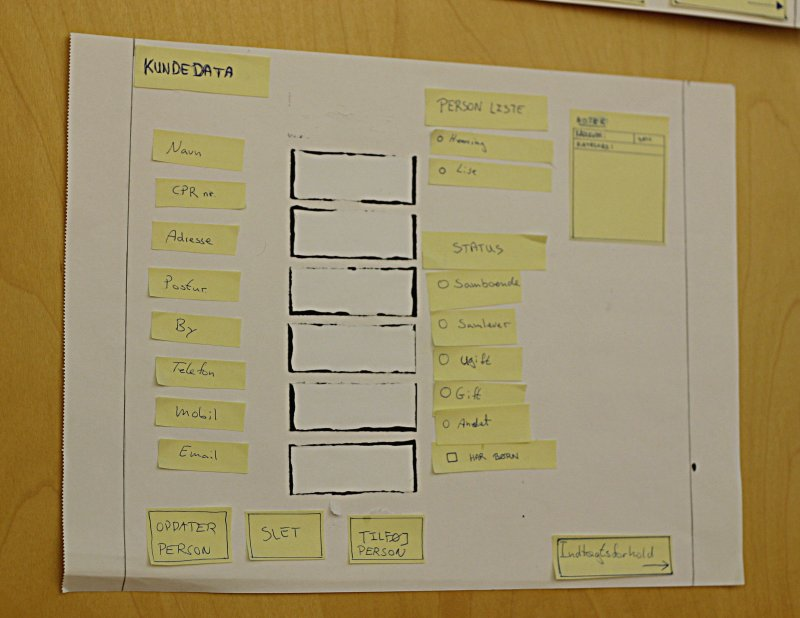
\includegraphics[width=1.00\textwidth]{Billeder/Prototype_Praecisering_Stills/Session1/PT1_KundeData2.jpg}
\caption{Prototype 1, KundeData}
\label{PT1_KundeData}
\end{figure}

\begin{figure}
\centering
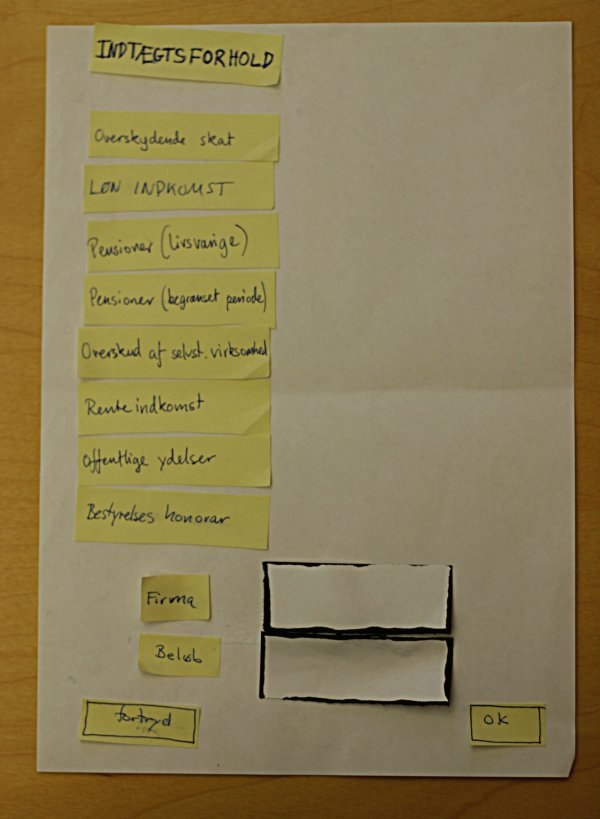
\includegraphics[width=1.00\textwidth]{Billeder/Prototype_Praecisering_Stills/Session1/PT1_IndtaegtForholdPopup.jpg}
\caption{Prototype 1, IntaegtForhold popup}
\label{PT1_IntaegtForholdPopup}
\end{figure}

\begin{figure}
\centering
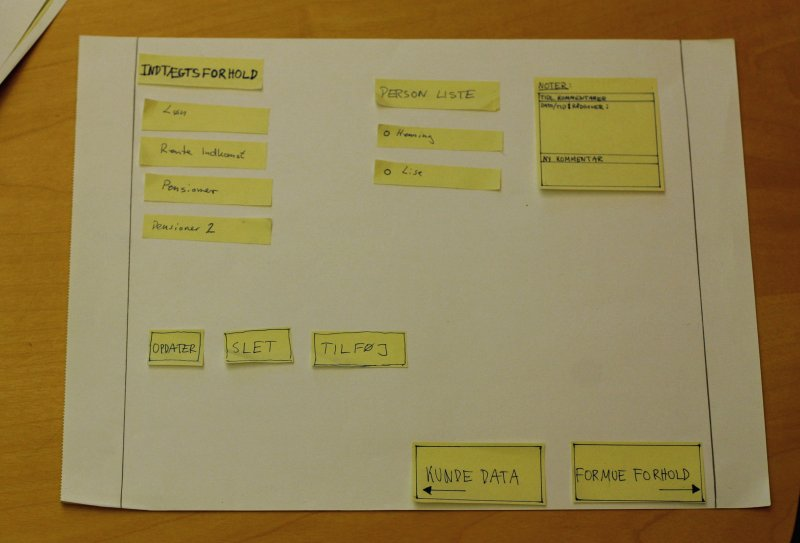
\includegraphics[width=1.00\textwidth]{Billeder/Prototype_Praecisering_Stills/Session1/PT1_IntaegtForhold2.jpg}
\caption{Prototype 1, IntaegtForhold}
\label{PT1_IntaegtForhold}
\end{figure}

\item \textbf{Anden uge:}
Vi afholdte to sessioner med den f�rste prototype, hvor m�let var at f� indsamlet krav til systemet, se afsnit \ref{Kravliste} p� side \pageref{Kravliste}. Sessionerne blev dokumenteret ved hj�lp af video og notetagning. Ugen blev ogs� brugt til at analysere de selvsamme krav, og s� fik vi et crash kursus i pensionsteori. Denne uges h�rde n�d var at indsamle krav og at f� en forst�else af EIK Banks verden. Derudover blev vi einge om at fredag fremover skulle v�re en dag hvor vi skrev rapport.


\item \textbf{Tredje uge:}
Vi konstruerede anden prototype og afholdte tredje prototype session. Foto fra sessionen kan ses p� side \pageref{prototype2_KundeData}, \pageref{prototype2_FormueForhold_popup1} og \pageref{prototype2_FormueForhold_popup2} 
Til denne session valgte vi at g�re brug af lyd\-optagelser og noter. Det var ogs� i denne uge at vi fandt ud af hvad vi skulle fokusere p� i vores rapport. Det vil sige at vi valge to studieomr�der, brugevenlige brugergr�nseflader og design patterns. 

\begin{figure}
	\centering
		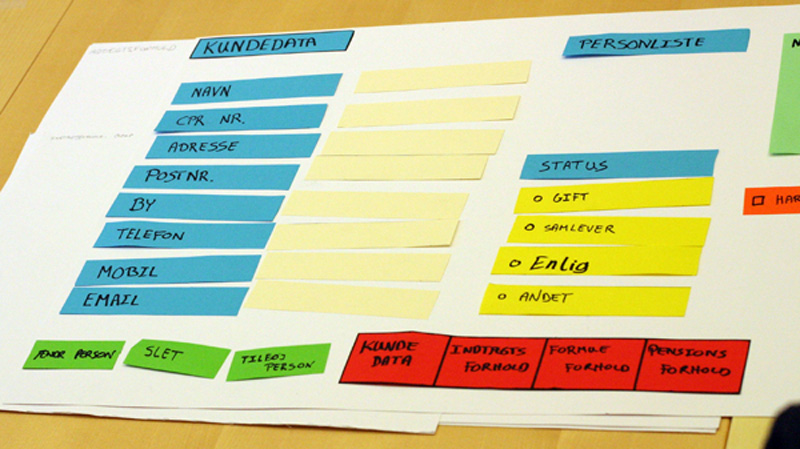
\includegraphics[width=1.00\textwidth]{Billeder/Prototype_Praecisering_Stills/PT2_KundeData1.jpg}
	\caption{Prototype 2, KundeData}
	\label{prototype2_KundeData}
\end{figure}

\begin{figure}
	\centering
		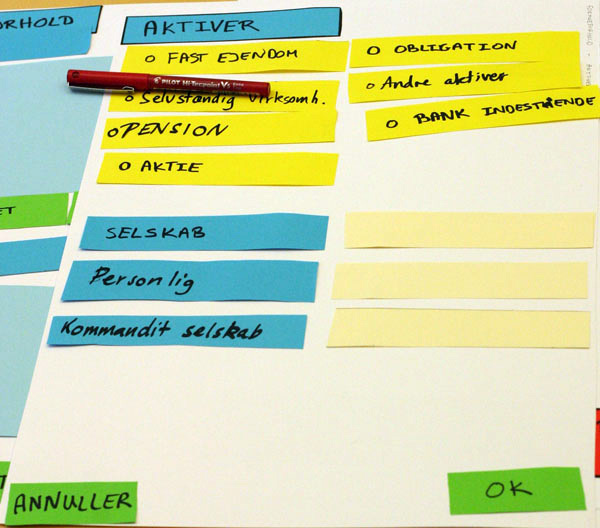
\includegraphics[width=1.00\textwidth]{Billeder/Prototype_Praecisering_Stills/PT2_FormueForholdPopupAktiv1.jpg}
	\caption{Prototype 2, FormueForhold popup}
	\label{prototype2_FormueForhold_popup1}
\end{figure}

\begin{figure}
	\centering
		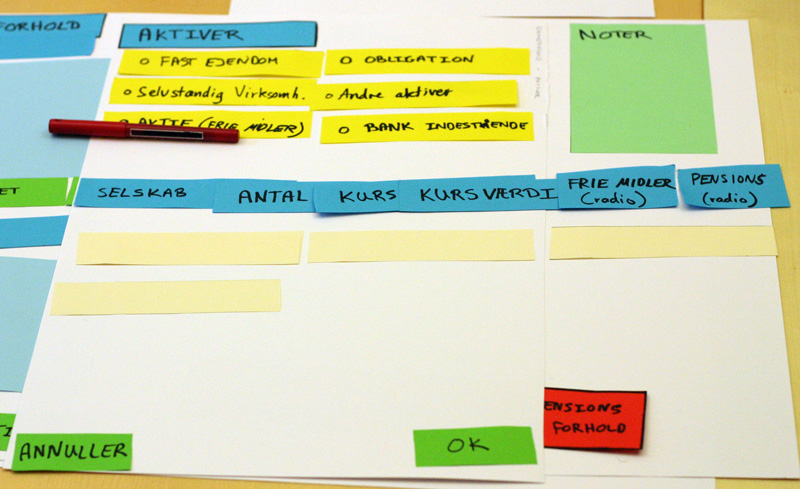
\includegraphics[width=1.00\textwidth]{Billeder/Prototype_Praecisering_Stills/PT2_FormueForholdPopupAktiv2.jpg}
	\caption{Prototype 2, FormueForhold popup 2}
	\label{prototype2_FormueForhold_popup2}
\end{figure}

\item \textbf{Fjerde uge:}
Denne uge omhandlede prim�rt sp�rgsm�l om design af det nye system. Vi identificerede klasser og lavede den overordnede arkitektur til systemet. Det udmyndigede sig i et klassediagram, hvilket kan ses i afsnit \ref{klassediagram} p� side \pageref{klassediagram}. Vi fik lavet en testapplikation som gjorde brug af design patternet Model View Controller. Dette kan der l�ses mere om i afsnit \ref{design_pattern} p� side \pageref{design_pattern}. Denne test var grundlaget for arkitekturen i systemet. Denne uges h�rde n�d gik ud p� at f� kodet en lille applikationen som kunne l�se og skrive til en Access database. Denne applikation skulle derfor testes p� en af EIK Banks computere og alt gik godt. Testen kan l�ses i afsnit \ref{Test af database tilgang} p� side \pageref{Test af database tilgang}. Det var ogs� i denne uge at lavede et strukturdokument der fort�ller om navnekonventioner i koden.

\item \textbf{Femte uge:}
Ugen gik med med at programmere sidste uges fastlagte arkitektur. Vi diskuterede hvordan og hvorledes med performance og database. Diskutionen kan l�ses i afsnit \ref{databasePerformence} p� side \pageref{databasePerformence}. Der var i denne uge ikke nogen n�d, ud over det faktum, at der var kilometer vis af kode der skulle kodes og der naturligvis ikke var tid nok i d�gnet.

\item \textbf{Sjette uge:}
Vi programmerede forsat p� livet l�s, men til forskel fra sidste uge fokuserede vi mere p� at f� koden til at virke sammen med de brugergr�nseflader vi havde lavet. Det var ogs� i denne uge at vi blev enige om at begynde at kode brugergr�nsefladen til 'indt�gter' og 'kunde' helt igennem, for s� at kunne bruge den som skabelon for de resterende brugergr�nseflader. P� den m�de kunne vi n�jes med at lave fejl �t sted og dermed f� vigtige kodem�ssige erfaringer, som s� i fremtiden kunne bruges p� de andre sk�rme. Den h�rde n�d gik igen fra sidste uge. 

P� den ugentlige fredagsbriefing pr�senterede vi EIK Bank for en afgr�nsning, som gik ud p� at udlade printfunktionaliteten i systemet. Det var EIK Bank ikke enige i og dermed blev vores plan �ndret og vi fandt lige pludselig en ny h�rd n�d.

\item \textbf{Syvende uge:}
Som reaktion p� sidste uges fredagsm�de arrangerede vi et m�de med EIK Bank hvor vi kvantificerede en del af kravene. Vi kom ogs� igang med den h�rdeste n�d, det vil sige udprintning, fik unders�gt emnet p� nettet og konsulteret en l�rer p� skolen. Vi fik til dels implementeret regler for brugergr�nsefladen, p� en s�dan m�de at brugeren ikke kan komme til at lave ulykker.

\item \textbf{Ottene uge:}
Vi arbejdede h�rdt p� at f� kn�kket den h�rdeste n�d, udprintning. Se afsnit \ref{udprint} p� side \pageref{udprint}. Den formatering, som vi var blevet enige med EIK Bank om, voldte os store problemer og vi blev internt i gruppen enige om at lave �n printfunktion som virkede, frem for at lave noget halvf�rdigt som ikke virkede. Det betyder at vi kun til dels har f�et kn�kket n�dden. Vi kan printe, men ikke helt som vi gerne skulle. Vi fik ogs� finpudset de sidste ting i koden, lavet sk�rmene 'KundeData' og 'Indtaegt' f�rdige og vi fik skrevet kommentarer de steder hvor koden var f�rdig. Det var ogs� i denne uge af vi lukkede for videreudvikling p� systemet, for herefter at fokusere p� rapport skrivning.

\item \textbf{Niende uge:}
Den h�rdeste n�d nu at skrive rapport og f� den f�rdig. Vi fik ogs� lavet en test session hvor vi ville se, om der var potentiale i vores system, ang�ende kravet om hvor lang tid det m� tage at indtaste kunde oplysninger. Vi fik afleveret en forel�belig rapport til EIK Bank s� de kunne l�se den igennem og se at vi ikke har skrevet noget inkriminerende om EIK Bank.

\item \textbf{Tiende uge:}
Der var stadig en del der skulle skrives til rapporten og det blev gjort. Diagrammer, sk�rmbilleder og s� videre blev gjort f�rdige og klar til at komme i rapporten. Nu da rapporten er f�rdig er den sidste h�rde n�d kn�kket.
\end{itemize}


\section{Eksempel p� dokumentation}
EIK Bank har udtrykt �nske om at vi, i udviklingsperioden, fokuserer p� funktionalitet i applikationen, fremfor dokumentation af systemet. For at give et eksempel p� dokumentation af applikationens funktionalitet, har vi valgt at gennemg� hvordan vi opretter en indt�gt, fra start til slut. Vi vil her vise relevante diagrammer, fra krav og usecase-, til klasse- og sekvensdiagrammer og demonstrere funktionens kald ned gennem arkitekturens lag. Dermed giver vi ogs� et indblik i hvordan vores arkitektur h�nger sammen.

Dokumentation er ikke helt uv�sentlig n�r der udvikles software til en bank. N�r en bank vil tage et edbsystem i brug skal det godkendes af Finanstilsynet. Det betyder at banken skal dokumentere systemet efter g�ldende lovgivning.

Ud fra de fastlagte funktionelle krav om hvad applikationen skal kunne, ses det blandt andet at programmet skal kunne tilf�je, se, slette og redigere en indt�gt i et kundeforhold. Udf�relsen af dette krav sker i forbindelse med indtastningen af kundens forhold. Kravet er fundet ved at se p� hvilke kundeforhold der findes i EIK Banks nuv�rende system. Vi har til dette eksempel valgt at bruge del\-kravet 'tilf�j indt�gtsforhold', og som indt�gtsforhold bruger vi aktieindkomst. Kravet st�r som nummer 20 p� kravlisten og ud fra det kan vi definere f�lgende usecase, se figur \ref{fig:IndtaegtUsecase} p� side \pageref{fig:IndtaegtUsecase}.

\begin{figure}
	\centering
		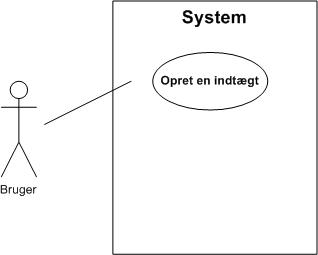
\includegraphics{Billeder/IndtaegtUsecase.jpg}
	\caption{Usecase Indtaegt}
	\label{fig:IndtaegtUsecase}
\end{figure}

Funktionen ligger i klassen 'Indtaegt' og er navngivet \textit{GemIndtaegt()}. Klassen 'Indtaegt' er abstrakt, hvilket betyder at man ikke kan instantiere klassen, vi instantierer subklasserne og ikke superklassen. Metoden \textit{GemIndtaegt()} er virtuel, hvilket betyder at de klasser der arver metoden, nemlig subklasserne, har mulighed for at overskrive funktionen. Se udsnittet af klassediagrammet, figur \ref{fig:ClassDiagramIndtaegt}, side \pageref{fig:ClassDiagramIndtaegt}.

Nedenst�ende arkitektur-diagram viser strukturen i applikationen, i forbindelse med 'Indtaegt', se figur \ref{fig:IndtaegtStruktur} p� side \pageref{fig:IndtaegtStruktur}. Der gives derudover et eksempel fra appliktionenen p� hvilken indflydelse design patternet MVC har p� vores arkitektur og den opdeling det i praksis medf�rer. Der kan l�ses om MVC i afsnit \ref{MVC} p� side \pageref{MVC}.

\newpage
\begin{figure}
	\centering
		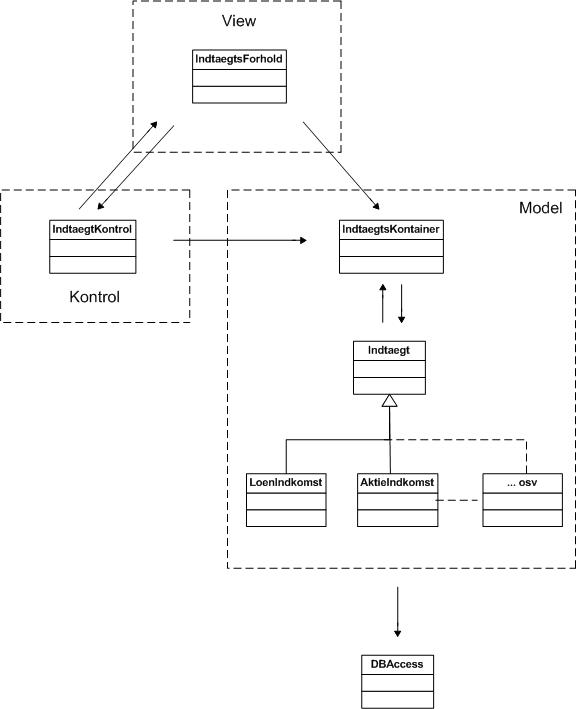
\includegraphics[width=1.0\textwidth]{Billeder/IndtaegtStruktur.jpg}
	\caption{System arkitektur}
	\label{fig:IndtaegtStruktur}
\end{figure}

F�lgende sekvensdiagram viser de specifikke kald i strukturen i forbindelse med at oprette en 'indtaegt', i dette tilf�lde en 'aktieindkomst', se figur \ref{fig:IndtaegtSekvens} p� side \pageref{fig:IndtaegtSekvens}. Af praktiske �rsager, hvilket vil sige pladsmangel p� siden, har vi valgt at springe visse kald over i diagrammet. Hele forl�bet beskrives i nedenst�ende gennemgang, hvor 2 til og med 5 er udeladt fra sekvensdiagrammet:

\begin{enumerate}
\item Brugeren opretter en ny indt�gt p� formen 'Indtaegter' (view) i applikationen. Dette g�res ved at trykke p� knappen 'Tilf�j'.
\item Formen 'Indtaegter' sender en event videre til kontrol klassen 'IndtaegtKontrol'.
\item 'Indtaegtkontrol' kalder, via eventhandleren, funktionen \textit{session.get\-Kunde()} for at opklare hvilken kunde der er valgt p� personlisten.
\item \textit{session.GetKunde()} kalder \textit{KundeKontainer.GetKunde()}, som returnerer kunde-objektet til 'IndtaegtsKontrol'.
\item Eventhandleren i 'IndtaegtKontrol' kalder nu \textit{Kunde.Gem\-Aktie\-Indkomst()} med udbytte og kursgevinst som parametre.
\item \textit{Kunde.GemAktieIndkomst()} kalder \textit{IndtaegtsKontanier.Gem\-Aktie\-Indkomst()}.
\item \textit{IndtaegtsKontainer.GemAktieIndkomst()} opretter nu en ny instans af 'AktieIndkomst', som f�r overf�rt parametrene til dens konstrukt�r. 
\item Derefter kaldes \textit{GemIndtaegt()} p� objektet 'AktieIndkomst'.
\item \textit{AktieIndkomst.GemIndtaegt()} starter med at kalde baseklassens \textit{GemIndtaegt()}.
\item \textit{Indtaegt.GemIndtaegt()} s�rger for at lave plads i tabellen 'Indtaegter' i databasen.
\item Derefter opdaterer \textit{AktieIndkomst.GemIndtaegt()} den oprettede tupel i databasen, med de data der skal gemmes for aktieindkomsten,
\item Til slut opretter \textit{IndtaegtsKontainer.GemAktieIndkomst()} objektet i datastrukturen, ved at tilf�je aktieindkomsten til den generiske liste af indtaegter.
\end{enumerate}

Ovenst�ende afspejler den algoritme vi har konstrueret til at gemme et kundeforhold. Algoritmen kan ses i 6 trin, p� side \pageref{gem-algoritme} under afsnittet \ref{gem-algoritme}.

\newpage

\begin{figure}
	\centering
		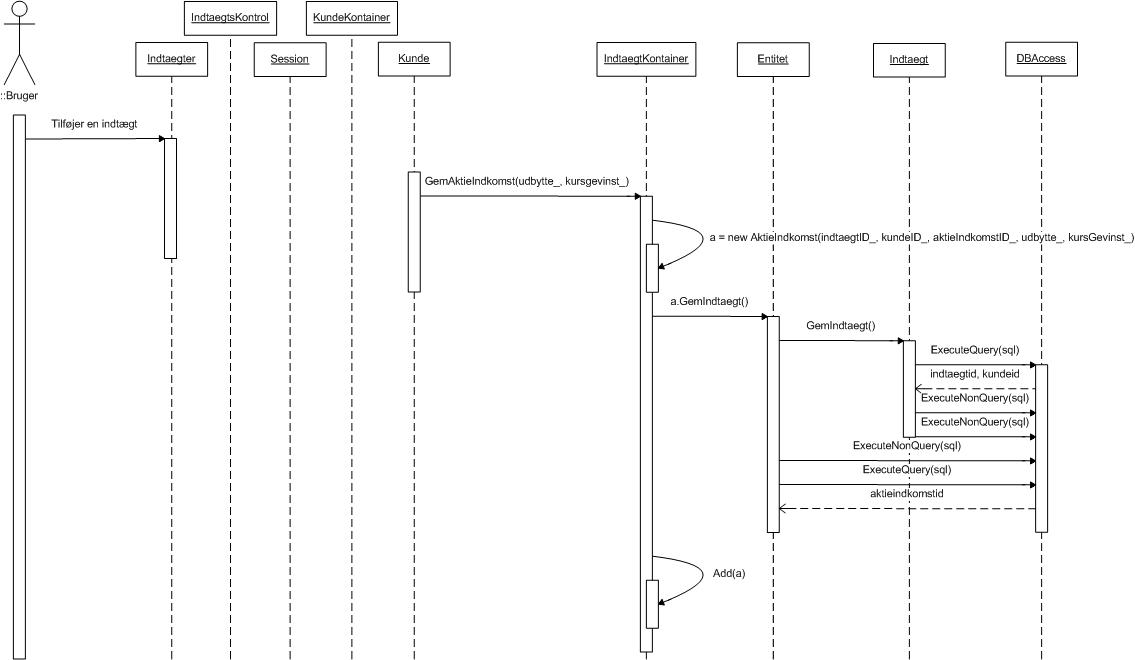
\includegraphics[angle=270, width=0.90\textwidth]{Billeder/IndtaegtSekvens.jpg}
	\caption{Sekvensdiagram GemIndtaegt}
	\label{fig:IndtaegtSekvens}
\end{figure}


\newpage
Her viser vi et udsnit af koden som underst�tter sekvensdiagrammet \ref{fig:IndtaegtSekvens} p� side \pageref{fig:IndtaegtSekvens}.
\lstset{language=[Sharp]C, % fort�ller hvilket sprog koden er skrevet i.
  basicstyle=\small, breaklines=true}
\begin{lstlisting}
public partial class Indtaegter : Form
{
  private void btnIndtaegterTilfoej_Click(object sender, EventArgs e)
  {
    indtaegtKontrol.getEvent(sender);
    set_false();
  }
}

//F�lgende er et resultat af at en bruger har trykket p� knappen tilf�j p� popup formen til 'Indtaegter'

public class IndtaegtKontrol
{
  private System.Windows.Forms.Button SenderBtn = null;
  
  private Indtaegtsforhold indtaegtForm;
  private Indtaegter indtaegtPopUpForm;
  private Session session;
  private Indtaegt.Indtaegt indtaegt;

  public void getEvent(object sender)
  {
    if (sender.GetType().Name == "Button")
    {
      //Her typecastes objektet 'sender' til typen 'Button'
      SenderBtn = (System.Windows.Forms.Button)sender;

      if (sender.GetType().Name == "Button")
      {
        SenderBtn = (System.Windows.Forms.Button)sender;
        if (SenderBtn.Name == "btnIndtaegterTilfoej" && SenderBtn.Text == "Tilf�j")
          {
          Kunde kunde = null;

          if (indtaegtForm.rdoPerson1.Checked)
          {
            kunde = session.GetKunde(0);
          }
          else if (indtaegtForm.rdoPerson2.Checked)
          {
            kunde = session.GetKunde(1);
          }
          indtaegtPopUpForm.Refresh();

          //Her springer vi lidt i funktionen for kun at vise det, for eksemplet, relevante kode. Det vil sige uvedkommende forgreninger er undladt.

          else if (indtaegtPopUpForm.rdoAktieIndkomst.Checked)
          {
            try
            {
              int udbytte = Convert.ToInt32(indtaegtPopUpForm.txtUdbytte.Text);
              int kursgevinst = Convert.ToInt32(indtaegtPopUpForm.txtKursGevinstTab.Text);
              kunde.GemAktieIndkomst(udbytte, kursgevinst);
            }
            catch (FormatException fe)
            {
              Console.WriteLine("IndtaegtKontrol.btnTilfoej : " + fe.Message);
            }
          }
          indtaegtForm.OpdaterTrae(kunde);
        }
      }
    }
  }
}

//F�lgende er et resultat af IndtaegtKontrol.kunde.GemAktieIndkomst(udbytte, kursgevinst);

public class Kunde
{
  private IndtaegtsKontainer indtaegter;
  
  public void GemAktieIndkomst(int udbytte_, int kursgevinst_)
  {
    indtaegter.GemAktieIndkomst(udbytte_, kursgevinst_);
  }
}

//F�lgende er et resultat af Kunde.indtaegter.GemAktieIndkomst(udbytte_, kursgevinst_);

public class IndtaegtsKontainer
{
  private List<Indtaegt> indtaegter;

  public void GemAktieIndkomst(int udbytte_, int kursgevinst_)
  {
    AktieIndkomst a = new AktieIndkomst(0, kundeID, 0, udbytte_, kursgevinst_);
    a.GemIndtaegt();
    indtaegter.Add(a);
  }
}                

//F�lgende er et resultat af kaldet IndtaegtsKontainer.a.GemIndtaegt();

public class AktieIndkomst : Indtaegt
{
  private int aktieIndkomstID;
  private int udbytte;
  private int kursGevinst;
 
  public override void GemIndtaegt()
  {
    ///Tilf�jer en entry i tabellen Indtaegt
    base.GemIndtaegt();
    ///Tilf�jer aktieindkomsten til tabellen aktieindkomst, med relation til 
    ///den indtaegt der blev tilf�jet ovenfor
    string sql = "INSERT INTO aktieindkomst (indtaegtid, udbytte, kursgevinst) values (" + base.IndtaegtID + "," + udbytte + "," + kursGevinst + ")";
    DBAccess.getDBInstance().ExecuteNonQuery(sql);

    ///Henter det p�g�ldende indtaegtid
    sql = "SELECT aktieindkomstid FROM aktieindkomst WHERE indtaegtid=" + base.IndtaegtID;
    DataSet myDataSet = DBAccess.getDBInstance().ExecuteQuery(sql);

    try
    {
      aktieIndkomstID = Convert.ToInt32(myDataSet.Tables["Result"].Rows[0][0].ToString());
    }
    catch (NullReferenceException nre)
    {
      Console.WriteLine("AktieIndkomst.GemIndtaegt 2 : " + nre.Message);
    }
  }
}

//F�lgende er et resultat af kaldet AktieIndkomst.base.GemIndtaegt();

public abstract class Indtaegt
{
  private int indtaegtID;
  private int kundeID;
        
  public virtual void GemIndtaegt()
  {
    ///Finder den tupel i tabellen indtaegt der er klar til brug (den med det h�jeste id)
    string sql = "SELECT indtaegtid, kunde.kundeid FROM indtaegt inner join kunde on indtaegt.kundeid = kunde.kundeid WHERE navn='Default'";
    DataSet myDataSet = DBAccess.getDBInstance().ExecuteQuery(sql);
    int emptyIndtaegtID = 0;
    int defaultKundeID = 0;
    try
    {
      emptyIndtaegtID = Convert.ToInt32(myDataSet.Tables["Result"].Rows[0][0].ToString());
      defaultKundeID = Convert.ToInt32(myDataSet.Tables["Result"].Rows[0][1].ToString());
    }
    catch (NullReferenceException nre)
    {
      Console.WriteLine("Indtaegt.GemIndtaegt 1 : " + nre.Message);
    }

    ///Inds�tter en ny tom tupel i indtaegt (id+1).
    sql = "INSERT INTO indtaegt (kundeid) VALUES (" + defaultKundeID + ")";
    DBAccess.getDBInstance().ExecuteNonQuery(sql);

    ///Opdaterer den (tomme) hentede tupel med det tilh�rende kundeID.
    sql = "UPDATE indtaegt SET kundeid=" + KundeID + " WHERE indtaegtid=" + emptyIndtaegtID;
    DBAccess.getDBInstance().ExecuteNonQuery(sql);
    this.IndtaegtID = emptyIndtaegtID;
  }
}

//F�lgende er et resultat af kaldet IndtaegtKontrol.indtaegtForm.OpdaterTrae(kunde);

public partial class Indtaegtsforhold : Form
{
  private IndtaegtKontrol indtaegtKontrol;
  private Session session;
        
  public void OpdaterTrae(Kunde k)
  {
    List<Indtaegt.Indtaegt> indtaegtListe = k.getIndtaegtKontainer().GetIndtageter();
            
    treeIndtaegter.Nodes.Clear();

    foreach (EIKBank.Indtaegt.Indtaegt i in indtaegtListe)
    {
      if (treeIndtaegter.Nodes.Count == 0)
      {
        TreeNode gren = new TreeNode(k.getIndtaegtKontainer().GetSumAfIndtaegt(i));
        treeIndtaegter.Nodes.Add(gren);
        TreeNode blad = new TreeNode(i.Praesenter());
        gren.Nodes.Add(blad);
      }
      else
      {
        bool found = false;
        foreach (TreeNode n in treeIndtaegter.Nodes)
        {
          if (n.Text.Equals(k.getIndtaegtKontainer().GetSumAfIndtaegt(i)))
          {
            found = true;
            TreeNode blad = new TreeNode(i.Praesenter());
            n.Nodes.Add(blad);
          break;
          }
        }
        if (found == false)
        {
          TreeNode gren = new TreeNode(k.getIndtaegtKontainer().GetSumAfIndtaegt(i));
          treeIndtaegter.Nodes.Add(gren);
          TreeNode blad1 = new TreeNode(i.Praesenter());
          gren.Nodes.Add(blad1);
        }
      }
    }
  }
}
\end{lstlisting}



\chapter{Tekniske l�sninger}
\section{Vores valg af udviklingsmilj�}

Vi har i gruppen hver is�r forskellige programmeringssprog som vi br�nder for og har arbejdet mest med. Nogle er til Java, nogle er til C\# og andre er til noget helt tredje. Dog havde vi den f�llesn�vner at alle i gruppen havde det samme valgfag p� 4. semester, nemlig .Net \& Visual Studio 2003. Her dannede vi ogs� gruppe, for at lave valgfagsprojekt i samme fag. I valgfagsprojektet skulle vi lave en applikation i Visual Studio 2003 og her valgte vi C\# som programmeringssprog. Vi skulle endvidere bygge en Access database og fik dermed �velse i at koble de to v�rkt�jer sammen.

Da vi begyndte p� hovedopgaven var .Net frameworket lige udkommet i version 2.0 og Visual Studio var udgivet i den nye version 2005. EIK Bank har ikke haft nogen pr�ferencer over for  hvilket sprog applikationen udvikles i, da de ikke selv har udviklere siddende i huset. Eneste anm�rkning fra bankens side var at vi godt m�tte tage videre\-udviklings\-muligheder med i overvejelserne. Derfor lod vi vores f�lles erfaring fra 4. semester v�re et af argumenterne for at v�lge .Net platformen og sproget C\#. Et andet argument var at vi gerne ville arbejde mere med .Net og C\# og l�re platformen bedre at kende, da den er ``oppe i tiden''. Derfor mener vi ogs� at vores valg er med til at ``fremtidssikre'' systemet, da banken engang i fremtiden med sikkerhed kan finde ekstern arbejdskraft til videreudvikling af systemet i og med at platformen er udbredt og anvendes mange steder.

\newpage
\section{Database}\label{Database}

Vi har brugt en del tid i l�bet af den f�rste uge p� af finde ud af hvilken databasel�sning vi kunne bygge EIK Banks nye system op omkring. Umiddelbart s� vi tre mulige l�sninger.

\begin{enumerate}
\item EIK Bank har i forvejen et samarbejde med SDC\footnote{Sparekassernes Data Central}, hvor SDC leverer alt det n�dvendige hardware og software. Vi t�nkte at SDC m�ske havde eller kunne s�tte en databaseserver op som applikation, som vi kunne k�re op imod. Det kunne de s�dan set godt, men det koster omkring 50.000,- i oprettelse og ca. 3.000,- om m�neden, og det ville s� v�re en IBM DB2 databaseserver. Det dur ikke, dels fordi at det er for dyrt (vi havde slet ikke t�nkt p� at det kostede penge) og dels fordi at DB2 er alt for stort i forhold til det vi skal bruge.
\item En anden l�sning kunne v�re at s�tte en lokal database server op i EIK Bank. Det har der ikke umidelbart v�ret stemning for. Det handler mest om at der ikke er ressourcer, i form af arbejdskraft, til at vedligeholde en s�dan server.
\item EIK Bank har hos SDC en filserver, som alle medarbejdere har adagang til. P� denne filserver kunne vi l�gge en databasefil, i form af en Access database.
\end{enumerate}

Konklusionen er at vi v�lger mulighed nr. 3. Dette er ikke det mest optimale valg, da der er flere problemer med Access.

For det f�rste er der en performancem�ssig faktor, hvor Access ikke leverer nogen s�rlig god ydelse.

Yderligere er der problemet med at en Access database, eftersom det bare er en fil, ikke tager h�nd om problemet med samtidig skrivning til samme data i databasen. Der er ikke nogen applikation der tager h�nd om, styrer og beskytter databasen.

Vi er st�dt p� flere, mere generelle, databaseproblematikker.
Under tilgang til databasen kan der opst� problemer. Problemet kaldes 'Lost Update': Konsulent 1 tager data om kunde X med ud til et m�de med kunde X og laver en masse rettelser.
Konsulent 2 tager, i dette tidsrum, adgang til databasen og laver nogle sm� rettelser i selvsamme data til kunde X og tilf�jer sine rettelser til den centrale database. Konsulent 1 kommer tilbage og vil nu uploade sine rettelser om kunde X, fra sin b�rbare computer til den centrale database. Problemet best�r i at de rettelser konsulent 2 har lavet, bliver overskrevet af konsulent 1. Og dermed vil en opdatering blive tabt. 

Problemet er if�lge EIK Bank ikke tilstede da to konsulenter aldrig arbejder p� de samme kunder. Det vil sige at der eksisterer et 1:1 forhold mellem konsulent og kunde. Vi m� derfor antage at sandsynligheden for at problemet skulle opst� i praksis er meget lille. Vi vil dog, som udviklere, mene at det er n�dvendigt at tage h�nd om problemet, da man ikke med hundrede procent sikkerhed kan afvise at problemet kan forekomme. Det er et fremtidsaspekt at den administrative afdeling skal st� for indtastningen, hvorfor man ikke kan afvise at en r�dgiver og en administrativ medarbejder kan komme til at tilg� samme kunde samtidigt.

N�r konsulenten er ude hos kunden kan konsulenten ikke vide om der vil v�re netadgang eller ej. Det betyder at konsulenten skal have data om kunden med hjemmefra. N�r konsulenten kommer hjem igen skal han l�gge de nye data ind i databasen. Vi kunne alts� lave en l�sning, som gemmer data lokalt p� computeren, n�r der ikke er kontakt med den centrale database. Den gemte data skal tilf�jes til den centrale database n�r r�dgiveren kommer tilbage til EIK Bank. Senere har vi t�nkt at r�dgiveren kan koble op til den centrale database med et mobilmodem. Denne l�sning kr�ver dog en del mere arbejde, i form af en webservice, der vil kr�ve en webserver.

\subsection{Mapping af database}
Med udgangspunkt i vores klassediagram skal vi have konstrueret en database. Dette g�r vi ved at 'mappe' fra vores konceptuelle model, hvilket vil sige vores klassediagram, til en relationel model. Til dette form�l benytter vi os af en 8 trins algoritme. Vi skal finde:

\begin{enumerate}
\item Regul�re klasser. Vi har regul�re klasser i form af Kunde, Indt�gt, Pension, Aktiv og Passiv.
\item Svage klasser og identificering af �n til mange (1:M) relationsforhold. Dem har vi ikke nogle af.
\item �n til �n (1:1) relationsforhold. Disse har vi ikke nogle af. Hvis vi ser p� klasse\-diagrammet ser vi (1:1) forhold mellem en entitet og en kontainer. Men da disse kontainerklasser ikke er regul�re klasser, skal der ses bort fra dette.
\item Regul�re (1:M) relationsforhold. En s�dan relation findes mellem Session og Kunde. Da Kunde er p� mange-siden, inkluderer vi Sessions prim�rn�glen som fremmedn�gle i Kunde. P� den m�de kommer Kunde til at pege p� den Session som kunden er en del af.
\item Mange til mange (M:N) relationsforhold. Disse har vi ikke nogle af.
\item Flerv�rdigede attributter. Disse har vi ikke nogle af.
\item Tern�re relationsforhold. Disse har vi ikke nogle af.
\item Udvidet klassediagram.
Dette g�r ud p� at mappe 'specialisering og generalisering' til databasen. Der er 4 forskellige m�der hvorp� vi kan g�re dette. Der tages udgangspunkt i den arv der er i Aktiv, som er superklassen, og de forskellige aktiver (aktier, obligationer mv.) som er subklasser.
\item[A] Vi har valgt denne model, hvor vi laver et relationsskema for hver klasse og inkluderer prim�rn�glen fra superklassen som fremmedn�gle i subklassen. Det har den fordel at vi ikke f�r redundant eller un�dige 'null' atributter.
\item[B] En anden version g�r ud p� at lave et relationsskema for hver subklasse. Dette giver problemer n�r der skal s�ges, da der i s� fald skal laves en join af subklasserne. Dette betyder at der skal s�ges i flere tabeller for at finde det man s�ger efter. Et andet problem er, at de data som subklasserne har til f�lles vil blive repr�senteret redundant. 
\item[C] En tredje l�sning er et relationsskema for superklassen med attributterne fra alle subklasserne, plus een attribut til at skelne mellem subklasserne. Denne l�sning bruges n�r der er tale om disjunkte attributter i subklasser, hvormed der menes forskellige, ikke-overlappende attributter. Problemet er her at der vil v�re un�digt mange null attributer
\item[D] En fjerde l�sning er et relationsskema for superklassen med attributterne fra alle subklasserne, plus en attribut der agerer som flag til alle subklasserne. Denne l�sning bruges n�r der er tale om overlappende attributter i subklasser. Der er de samme problemer som med punkt C. Vi kan med fordel g�re brug af denne model n�r Pensionsforhold og dens subklasser skal mappes. 
\end{enumerate}

\subsection{Hvordan skal vi indl�se data fra databasen\label{databasePerformence}}
Vi skal nu kigge p� hvordan vi kan konstruere tilgangen til databasen, i henhold til det at l�se data ind i datastrukturen, ved programmets opstart. Hvor meget skal der hentes fra databasen?
Skal det hele hentes p� en gang eller skal det deles op? Hvor ofte skal der hentes data? Disse er overordnede sp�rgsm�l som vi vil besvare i det efterf�lgende.

F�lgende algoritme beskriver hvorledes data hentes fra databasen og oprettes i datastrukturen.
\begin{enumerate}
\item Hent alle sessioner fra databasen.
\item Opret en session i datastrukturen.
\item Hent de personer, fra databasen, der h�rer til den session
\item Opret en person i datastrukturen.
\item Hent alle indt�gtsforhold, fra databasen der h�rer til den person.
\item Opret disse indt�gtsforhold i datastrukturen..
\item Hent alle formueforhold/Aktiver, fra databasen der h�rer til den person.
\item Opret disse formuefhold/Aktiver i datastrukturen..
\item Hent alle formueforhold/Passiver, fra databasen der h�rer til den person.
\item Opret disse formueforhold/Passiver i datastrukturen..
\item Hent alle pensionsforhold, fra databasen der h�rer til den person.
\item Opret disse pensionsforhold i datastrukturen..
\item Hvis der er flere kunder, g� til punkt 4.
\item Hvis der er flere sessioner, g� til punkt 2
\item F�rdig.
\end{enumerate}

Da EIKBank i skrivende stund har omkring 1500 sessioner og hver session har 1,5 person med hver 14 forskellige forhold, s� bliver det til 31500 kald til databasen. Dette skal kunne g�res mere effektivt, hvilket beskrives i de efterf�lgende afsnit.

Test af tilgangen til databasen.
\lstset{language=[Sharp]C, % fort�ller hvilket sprog koden er skrevet i.
  basicstyle=\small, breaklines=true}

\begin{lstlisting}
Public static void main(String[] args){
   Console.WriteLine(System.DateTime.Now);
   for (int i = 0; i < 10000; i++)
   {
      DBAccess.getDBInstance().ExecuteQuery("select * from kunde");
   }
   Console.WriteLine(System.DateTime.Now);
   Console.ReadKey();
}
\end{lstlisting}
\begin{verbatim}
start output : 20-02-2006 11:09:01
slut output  : 20-02-2006 11:16:53
\end{verbatim}

I ovenst�ende kode bliver databasen tilg�et 10.000 gange, samt at der er udskrevet start- og sluttidspunkt. Denne test er udf�rt med en OLEDB forbindelse. Databasen ligger p� samme maskine som koden. Det tog alts� 7 minutter og 52 sekunder. Det giver ca. 22,7 forsp�gelser pr sekund.
En loadtid p� sm� 8 minutter er selvsagt ikke tilfredsstillende og vi skal finde en bedre l�sning. 

En anden ting man kunne g�re var kun at l�se session og kunder ind fra databasen. Det giver s� kun 
$1500*1,5=2250$ tilgange til databasen, som vil tage 2250/22,7 = 1 minut og 40 sekunder, hvilket 
heller ikke er helt godt nok.

En tredje ting man kunne g�re er at hente alle sessionerne ind og oprette dem. Derefter hentes alle personerne fra databasen og man k�rer s� de $1500*1,5=2250$ gange gennem datastrukturen og opretter personerne. Det giver i alt to tilgange til databasen som tager under 1 sekund, men en k�retid i datastrukturen som siger $f(O)=Ln(2250)$, hvor det til de to f�rste metoder er $f(O)=1$. Det er denne metode vi vil bruge. F(O) er store o notation.

Senere skal alle kundens forhold hentes fra databasen, hvilket giver 21 (en for hver tabel) kald per kunde, men der hentes kun data for de kunder der er i en session. Det vil giver max 42 kald til databasen. Det giver os 44 kald til databasen og en forsinket opstart p� 2 sec. Hermed har vi n�et en mere realistisk tilgang til databasen.

Der er ikke noget krav fra kundens side om at systemet skal v�re hurtigt til at starte op. S� den eneste grund til at bruge krudt p� det her er, at det ikke er hensigtsm�ssigt at vente 5 min. p� at et program starter op. (Det forventes dog inddirekte at programmet har en "normal" responstid, hvilket vil sige at man h�jest skal vente i et par sekunder)

Med hensyn til en eventuelt fremtidig opgradering af databasen, er det et af kravene til systemet at det skal v�re tilpas modul�rt opbygget, s� kun DBAccess modulet skal �ndres. Dog er SQL-kaldene i flere tilf�lde specifikke for Microsoft, hvorfor ogs� SQL-kaldene skal revurderes og skrives om til normal SQL standard. Et eksempel p� dette er vores brug af ordet 'Session' som et tabelnavn i databasen. Da dette er et reserveret ord i OLEDB (Jet x.x) driveren, skal navnet i Microsoft SQL-s�tningen skrives som '[Session]'. Dette vil ikke virke med almindelig SQL-standard.

\subsection{Hvordan skal vi skrive data til databasen?}

En af grundene til at vi skal kigge n�rmere p� dette, er netop Access's problem med at den ikke tager h�jde for samtidighedsproblemet\footnote{samtidig skrivning til databasen}. Derfor er vi n�dsaget til selv at lave en konstruktion der beskytter os mod dette. Ud over dette skal vi igen overveje de performance- og sikkerhedsm�ssige forhold.

Der er to m�der at gribe sagen an p�:

\begin{enumerate}
\item Der gemmes kun n�r en session afsluttes.
\item Der gemmes hver gang for eksempel en 'aktie' eller en 'pension' bliver oprettet og/eller �ndret.
\end{enumerate}

For at sikre konsistensen i databasen, er der nogle skridt der skal tages. Man kunne for eksempel g�re det p� en s�dan m�de at der altid er en tom record i databasen, som altid har det h�jeste id. 

Det man s� skal g�re, n�r en ny post oprettes, er:
\begin{enumerate}
\item Fra databasen v�lges den tomme tupel, ved: SELECT id FROM tablenavn WHERE kolonnenavn='tom'; Den skal bruges til at gemme den nye post i.
\item Man inds�tter en ny tom tupel med et nyt max(id).
\item Man opdaterer den tupel med det tidligere max(id).
\item Hvis der er tale om at gemme hver gang en post oprettes, s� skal denne ogs� oprettet i datastrukturen.
\end{enumerate}

Herunder ses et eksempel p� hvordan koden ser ud til 'gem kunde'.
\lstset{language=[Sharp]C, % fort�ller hvilket sprog koden er skrevet i.
  basicstyle=\small, breaklines=true}

\begin{lstlisting}
public void SaveKunde(int sessionID_, string navn_, long cpr_, string adresse_, int postnr_, int telefon_, int mobil_, string email_, int civilStatus_, bool harBoern_)
{
//Finder den tomme post
  string sql = "SELECT kundeid FROM kunde WHERE navn='Empty'";
  DataSet myDataSet = new DataSet();
  myDataSet = DBAccess.getDBInstance().ExecuteQuery(sql);
  int kundeID = 0;
            
  try
  {
    kundeID = Convert.ToInt32(myDataSet.Tables["Result"].Rows[0][0].ToString());
  }
  catch (NullReferenceException nre)
  {
    Console.WriteLine(nre.Message);
  }
            
  String getDefaultSessionIDSql = "SELECT sessionid FROM [session] WHERE raadgiver = 	'Empty'";
  myDataSet = new DataSet();
  myDataSet = DBAccess.getDBInstance().ExecuteQuery(getDefaultSessionIDSql);
  int defaultSessionID = 0;
            
  try
  {
    defaultSessionID = Convert.ToInt32(myDataSet.Tables["Result"].Rows[0][0].ToString());
  }
  catch (NullReferenceException nre)
  {
    Console.WriteLine(nre.Message);
  }
            
  //Oprette en ny tom post
  String setTomtObjekt = "INSERT INTO kunde(navn, sessionid, postnr) VALUES ('Empty'," + defaultSessionID + ", 800)";
  Console.WriteLine(DBAccess.getDBInstance().ExecuteNonQuery(setTomtObjekt).ToString());
	
  //Opdatere den tidligere tomme post
  sql = "UPDATE kunde SET sessionid="+sessionID_+", navn='"+navn_+"', cpr="+cpr_+", adresse='"+adresse_+"', postnr="+postnr_+", telefon="+telefon_+", mobil="+mobil_+", 	email='"+email_+"', civilstatus="+civilStatus_+", harboern="+harBoern_+" where 	kundeid="+kundeID;
  Console.WriteLine(DBAccess.getDBInstance().ExecuteNonQuery(sql));

  //S�tter ind i datastrukturen.
  addKunde(sessionID_, kundeID, navn_, cpr_, adresse_, postnr_, telefon_, mobil_, email_, civilStatus_, harBoern_);
}
\end{lstlisting}

Denne algoritme virker kun n�r en kunde skal oprettes i databasen. Skal vi derimod oprette en 
indt�gt, et aktiv eller et passiv, s� skal algoritmen v�re anderledes.

Den ser s�dan ud.\label{gem-algoritme}:
\begin{enumerate}
\item V�lg DEN Indt�gt som peger p� kunden med navnet 'Default'.
\item Opret en ny Indt�gt der peger p� kunden med navnet 'Default' (der er nu 2 tomme tupler).
\item Opdater indt�gten fra trin 1 s� den peger p� den aktuelle kunde.
\item Opret for eksempel en AktieIndkomst, som peger p� Indt�gten fra trin 1.
\item V�lg den AktieIndkomst som peger p� Indt�gten fra trin 1.
\item Opret AktieIndkomsten i datastukturen.
\end{enumerate}

Herunder ses et eksempel p� 'gem aktieindkomst'.
\lstset{language=[Sharp]C, % fort�ller hvilket sprog koden er skrevet i.
  basicstyle=\small, breaklines=true}

\begin{lstlisting}
public override void GemIndtaegt()
{
//trin 1
  string sql = "SELECT indtaegtid, kunde.kundeid FROM indtaegt inner join kunde on indtaegt.kundeid = kunde.kundeid WHERE navn='Default'";
  DataSet myDataSet = DBAccess.getDBInstance().ExecuteQuery(sql);
  int indtaegtID = 0;
  int kundeID = 0;

  try
  {
    indtaegtID = Convert.ToInt32(myDataSet.Tables["Result"].Rows[0][0].ToString());
    kundeID = Convert.ToInt32(myDataSet.Tables["Result"].Rows[0][1].ToString());
  }
  catch (NullReferenceException nre)
  {
    Console.WriteLine("AktieIndkomst.GemIndtaegt 1 : " + nre.Message);
  }

//trin 2
  sql = "INSERT INTO indtaegt (kundeid) VALUES (" + kundeID + ")";
  DBAccess.getDBInstance().ExecuteNonQuery(sql);

//trin 3
  sql = "UPDATE indtaegt SET kundeid=" + KundeID + " WHERE indtaegtid=" + indtaegtID;
  DBAccess.getDBInstance().ExecuteNonQuery(sql);

//trin 4
  sql = "INSERT INTO aktieindkomst (indtaegtid, udbytte, kursgevinst) values ("+indtaegtID+","+udbytte+","+kursGevinst+")";
  DBAccess.getDBInstance().ExecuteNonQuery(sql);

//trin 5
  sql = "SELECT aktieindkomstid FROM aktieindkomst WHERE indtaegtid="+indtaegtID;
  myDataSet = DBAccess.getDBInstance().ExecuteQuery(sql);

  try
  {
    aktieIndkomstID = Convert.ToInt32(myDataSet.Tables["Result"].Rows[0][0].ToString());
  }
  catch (NullReferenceException nre)
  {
    Console.WriteLine("AktieIndkomst.GemIndtaegt 2 : " + nre.Message);
  }

  IndtaegtID = indtaegtID;
  AktieIndkomstID = aktieIndkomstID;
}

public void GemAktieIndkomst(int udbytte_, int kursgevinst_)
{
  AktieIndkomst a = new AktieIndkomst(0, kundeID, 0, udbytte_, kursgevinst_);
  a.GemIndtaegt();
//trin 6
  indtaegter.Add(a);
}
\end{lstlisting}

Denne konstruktion sikrer at chancen for at to personer gemmer samtidigt p� samme id, er blevet meget lille. Den g�r ogs� det at der altid er et tomt id at gemme p�. Den g�r det ogs� muligt at oprette en entitet i datastrukturen med alle attributter. Alternativet er selv at skulle fasts�tte id'er, men s� skal man selv holde styr p� hvem der kan oprette hvilke id'er og hvilken v�rdi de skal have, for ikke at komme til at oprette to ens id'er. Et andet alternativ er at inds�tte sin data i databasen for s� at hente den ud igen med det, fra databasen oprettede, nye id. Problemet er her at man ikke ved hvilket id entiteten har f�et, da der kan v�re flere som gemmer samtidigt. N�r man s� sp�rger efter den med max(id) risikerer man at f� fat i den forkerte entitet. Hvis ikke der gemmes n�r en entitet er oprettet, s� f�r den ikke noget id og s� kan det blive sv�rt at identificere objektet i datastrukturen. For at summere op, s� har vi valgt at gemme data i databasen hver gang man i programmet opretter en entitet, og samtidig at oprette denne i datastrukturen. Dette betyder at vi benytter os af de to algoritmer som er beskrevet ovenfor.

\subsection{Normalisering af databasen}

N�r vi nu har f�et lavet vores database, er det tid til at se p� om den er konstrueret p� en hensigtsm�ssig m�de. Med hensigtsm�ssigt menes om den logiske databasestruktur er optimeret mest muligt. Det vil sige at finde betydningen af data og sammenh�ngen mellem disse. Vi skal finde og fjerne redundant data, og vi skal sikre entydig identifikation af data. Det er ogs� hensigtsm�ssigt at se p� mulige fremtidige �ndringer, og i den sammenh�ng at se p� om det er nemt eller sv�rt at udvide med en alternativ database. 

For at vi kan g�re disse ting skal vi unders�ge betydningen af data. For eksempel kan vi se p� hvad en kunde er i EIK Banks verden. Kort sagt best�r en kunde at persondata og fra nul til mange indt�gter, formueforhold og pensioner. Kundetabellen, som kan ses nedenfor, er ogs� et godt eksempel p� en tabel hvor man typisk kan finde redundant data. Redundant data forkommer n�r to eller flere kunder har adresse i samme by og postnr. Det giver problemer n�r det ut�nkelige sker, at en by skifter navn eller at byen skifter postnr. Det betyder at opdateringen af disse 
data kan resultere i inkonsistent data. Til at hj�lpe os med at optimere en logisk datastruktur g�r vi brug af normalisering. Normalisering forg�r i flere trin, startende fra f�rste normalform til femte normalform og hvert trin sikrer at visse problemer ikke kan opst�. N�r en database for eksempel er normaliseret efter tredie normalform, s� opfylder den ogs� f�rste og anden normalform.

For at vores database kan siges at opfylde 1. normalform skal
hver tupel have en entydig identifikation\footnote{l�s: n�gle}. Det betyder at en delm�ngde af identifikationen ikke alene m� kunne bruges som identifikation. Alle felter skal v�re atomariske, hvilket vil sige at de ikke m� indeholde lister, arrays med flere. Det betyder ogs� at der ikke m� v�re en repeterende delm�ngde af felter i en tupel. Der skal v�re en fast tupel l�ngde. Til hver tabel skal der v�re en fast tupel type. Det vil sige at en tupel i en tabel altid skal best� af de samme felter.

De to sidste punkter kan vi ikke undg� at opfylde. Til session har vi valgt at lave et sessionid som identifikation p� en tupel. Da en r�dgiver sagtens kan v�re en del af flere sessioner samme dag med samme tomme note, kan vi ikke bruge nogle eller en kombination af disse felter som identifikation. Derfor bruger vi sessionid som identifikation og derved er f�rste punkt opfyldt. Session indeholder ikke nogle lister, hvormed andet punkt ogs� er opfyldt.

For at opfylde 2. normalform skal databasen v�re p� 1. normalform, og
alle ikke-identifikationsfelter skal v�re afh�ngige af hele identifikationen. Det betyder at hvis 
der er en identifikation som er sammensat af flere felter, s� skal ikke-identifikationsfelterne v�re afh�ngige af alle identifikationsfelterne.

Da vi ikke har nogle sammensatte identifikationer opfylder vores database 2. normalform.

For at opfylde 3. normalform skal databasen v�re p� 2 normalform, og alle ikke-identifikationsfelter m� ikke v�re transitivt afh�ngige af identifikationen. Dette betyder at et felt i en tabel er afh�ngig af et andet felt i anden tabel, som s� er afh�ngig at identifikationen.

Et klassisk skoleeksempel p� dette er postnr og by problematikken, hvor by er afh�ngig af postnr, som igen er afh�ngig af identifikationen. Dermed er By transitivt afh�ngig af KundeID. Det man g�r, og som vi ogs� har gjort, er at skille by ud i en tabel for sig med identifikationen postnr. Postnr i kunde-tabellen laver vi om til en fremmedidentifikation.

Nedenfor ses et udsnit af vores tabeller.

\lstset{language=SQL, % fort�ller hvilket sprog koden er skrevet i [dialekt].
  basicstyle=\small, breaklines=true}

\begin{lstlisting}
CREATE DATABASE eikbank;

CREATE TABLE session(
  sessionid  AUTOINCREMENT PRIMARY KEY,
  raadgiver  TEXT,
  dato       TEXT, //Her kunne vi brugt et 'date' istedet for text, men det giver tit for mange problemer med computer installationer, programmeringssprog og databaser.
  note       TEXT
);

CREATE TABLE kunde(
  kundeid     AUTOINCREMENT PRIMARY KEY,
  navn        TEXT,
  cpr         LONGINT,
  adresse     INT,
  postnr      INT FOREIGN KEY REFERENCES postnr,
  telefon     INT,
  mobil       INT,
  sessionid   INT FOREIGN KEY REFERENCES session,
  civilstatus INT,
  harboern    BOOL
);

CREATE TABLE postnr(
  postnr  AUTOINCREMENT PRIMARY KEY,
  by      TEXT          NOT NULL
);
\end{lstlisting}

Et andet sted i databasen hvor der har v�ret problemer, er i tabellerne 'Aktie' og 'Obligation'.

\lstset{language=SQL, % fort�ller hvilket sprog koden er skrevet i [dialekt].
  basicstyle=\small, breaklines=true}

\begin{lstlisting}
CREATE TABLE aktiv(
  aktivid AUTOINCREMENT PRIMARY KEY
  kundeid int           FOREIGN KEY REFERENCES kunde
);

CREATE TABLE aktie(
\end{lstlisting}
  \vdots
\begin{lstlisting}
  antal      INT,
  kurs       INT,
  kursvaerdi INT,
\end{lstlisting}
  \vdots
\begin{lstlisting}
);

CREATE TABLE obligation(
\end{lstlisting}
  \vdots
\begin{lstlisting}
  antal      INT,
  kurs       INT,
  kursvaerdi INT,
\end{lstlisting}
  \vdots
\begin{lstlisting}
);

\end{lstlisting}

I og med at $kurs*antal=kursv�rdi$ kan vi fjerne $kursv�rdi$ fra tabellerne og lade applikationen regne kursv�rdien ud n�r den p�g�ldende form bliver genereret. Det er ikke hensigtsm�ssigt at gemme en sum, som kan regnes ud fra de to andre tal, s� l�nge at summen ikke skal bruges til noget senere. Vi har alts� her fjernet redundant data, hvilket forhindrede tabellerne $aktie$ og $obligation$ i at opfylde 1. normalform.
 
%Det vil sige at vi har redundant data i tabellerne, og dermed opfylder disse to tabeller ikke 1. normalform. Den simple l�sning er at slette kursvaerdi fra tabellerne og lade applikationen udregne denne ud fra kurs og antal.

Her stopper det for vores vedkommende. Man kunne g� videre med Boyes-Codd normalform og 4. og 5. normalform. Generelt kan man sige at man dekomponerer (nedbryder) sine tabeller n�r man normaliserer sin database. Problemet med 4. og 5. normalform er at de tager sig af problemer som kun opst�r i meget komplekse databaser. Der kan v�re problemer ved at bruge Boyes-Codd normalform i kraft af det ikke altid er muligt at g� tilbage til et tidligere trin (3. normalform). Disse mulige problemer og begrundelser g�r at vi stopper efter 3. normalform.

\subsection{Start-ops�tning af databasen}
For at applikationen skal kunne virke skal der v�re noget data i databasen. Uden denne data vil algoritmerne til at gemme kunder, indt�gter, aktiver og passiver ikke virke. I n�ste afsnit er 'x', 'y', 's', 't', 'o', 'p' og 'q' er naturlige tal og deres v�rdiger bliver automatisk sat i prim�rn�glen af databasen. Man skal selv huske at s�tte de rigtige fremmedn�gler. Tallet 'r' er lidt specielt da dette er et faktisk postnr og skal tastes ind manuelt. 

\begin{center}
\begin{table}[pbt]
\begin{tabular}{|l|l|l|l|}
\hline
\multicolumn{4}{|l|}{Session}\\ \hline
\underline{SessionID} & Raadgiver & Dato & Note \\ \hline
$x>0$ & Default & & \\ \hline
$y>0, y \neq x$ & Empty   & & \\ \hline
\end{tabular}
\caption{Session Tabel\label{session tabel}}
\end{table}

\begin{table}[pbt]
\begin{tabular}{|l|l|l|l|}
\hline
\multicolumn{4}{|l|}{Kunde}\\ \hline
\underline{KundeID} & Navn & Postnr & SessionID \\ \hline
$s>0$           & Default & 800 & x \\ \hline
$t>0, t \neq s$ & Empty   & 800 & y \\ \hline
\end{tabular}
\caption{Kunde tabel\label{kunde tabel}}
\end{table}

\begin{table}[pbt]
\begin{tabular}{|l|l|}
\hline
\multicolumn{2}{|l|}{Intaegt}\\ \hline
\underline{IndtaegtID} & KundeID \\ \hline
$o>0$ & s \\ \hline
\end{tabular}
\caption{Indtaegt tabel\label{indtaegt tabel}}
\end{table}

\begin{table}[pbt]
\begin{tabular}{|l|l|}
\hline
\multicolumn{2}{|l|}{Aktiv}\\ \hline
\underline{AktivID} & KundeID \\ \hline
$p>0$ & s \\ \hline
\end{tabular}
\caption{Aktiv tabel\label{aktiv tabel}}
\end{table}

\begin{table}[pbt]
\begin{tabular}{|l|l|}
\hline
\multicolumn{2}{|l|}{Passiv}\\ \hline
\underline{PassivID} & KundeID \\ \hline
$q>0$ & s \\ \hline
\end{tabular}
\caption{Passiv tabel\label{passiv tabel}}
\end{table}

\begin{table}[pbt]
\begin{tabular}{|l|l|}
\hline
\multicolumn{2}{|l|}{Postnr}\\ \hline
\underline{Postnr} & By \\ \hline
800 & H�je Taastrup\\ \hline
\end{tabular}
\caption{Postnr tabel\label{postbr}}
\end{table}
\end{center}

\subsection{Sikkerhed}
En af de ting vi ikke har kigget s� meget p� er transaktionsstyring. Transaktionsstyring er ikke helt uv�senligt n�r vi kigger p� vores gem algoritme, se afsnit \ref{gem-algoritme} p� side \pageref{gem-algoritme}. Da databasen tilg�es fem gange pr. genneml�b er der mange ting som kan g� galt. Hvis der g�r noget galt et sted, s� fejler hele algoritmen. I s�dan et tilf�lde hvor der er skrevet noget, men ikke det hele, til databasen, ville det v�re mest praktisk at lave et rollback. Det vil sige at skrive databasen tilbage til tilstanden f�r man begyndte at skrive. 
Nedenfor ses et eksempel p� hvordan dette kunne implementeres. F�lgene kode er pseudokode.
\lstset{language=[Sharp]C, % fort�ller hvilket sprog koden er skrevet i.
  basicstyle=\small, breaklines=true}
\begin{lstlisting}
IDbTransaction trans = null;
try{
  trans = connnection.BeginTransaction(IsolationLevel.Serializable);
  Gem algoritmen
  trans.Commit();
}
catch(exception e){
  trans.Rollback();
  Console.WriteLine(e.messege);
}
\end{lstlisting}
\newpage
\section{Udprintsfunktionalitet\label{udprint}}

\subsection{Indledende overvejelser}

Ud fra kravet fra EIK Bank om at systemet skal kunne printe en p�n rapport ud til kunden, har vi unders�gt hvilke muligheder vi har for at l�se denne opgave. Vi var alle i gruppen uerfarne med det at konstruere print-funktionalitet, hvorfor en del research af omr�det var n�dvendig.

Vi lagde fokus p� udprint-funktionaliteten i de sidste to uger af den tid vi havde til at udvikle systemet i. Det f�rste vi gjorde var at unders�ge muligheden for selv at konstruere en udprint-konstruktion, via de print-libraries der ligger i Visual Studio. Vi fandt dog hurtigt ud af at denne konstruktion ville blive temmelig kompliceret og kr�ve rigtig meget tid at lave. Kodeomfanget ville blive voldsomt og det at researche og finde ud af hvordan det kunne g�res, ville blive meget omfangsrigt. Vi konstruerede, til form�let, en helt simpel test-applikation, hvor vi printede en variabel fra datastrukturen ud. Dette virkede fint, men der er lang vej fra en simpel variabel til en konstruktionen af en f�rdig rapport.

Da vi ikke f�lte at dette var den rigtige l�sning, begyndte vi at se p� alternative muligheder. Vi unders�gte om der allerede findes v�rkt�jer skabt til at l�se problemet. Til det form�l fandt vi, via hj�lp fra en l�rer p� Niels Brock, v�rkt�jet Crystal Reports. Crystal Reports er et komponentbaseret rapporteringsv�rkt�j til .Net, med andre ord en udskriftsgenerator der kan lave formularer med datafelter fra databasen eller fra datastrukturen. Med dette v�rkt�j kan man konstruere og designe en rapport ud fra de data man har i sin applikation, hvor den resulterende rapport minder meget om et pdf-dokument. Der er inkluderet udprint-funktionalitet i v�rk�tjet, hvormed printproblematikken er l�st for vores vedkommende, da man kan printe rapporten ud, ved et simpelt tryk p� en knap. Hermed kan programmet ogs� levere en digital udgave af rapporten p� sk�rmen, f�r man printer, hvilket var et �nske fra EIK Banks side.

Crystal Reports viste sig rent faktisk at v�re inkluderet i Visual Studio 2005, det udviklingsmilj� som vi har brugt til udviklingen af applikationen. S� til form�let, syntes Crystal Reports at v�re den perfekte l�sning. B�de i henhold til vores problem med selve funktionaliteten, men ogs� i forhold til EIK Banks behov.


\subsection{V�rkt�jet Crystal Reports}

Crystal rapporten bliver genereret runtime, det vil sige n�r programmet k�rer og brugeren p� et tidspunkt beder om at f� rapporten lavet. 

Rapporten tilf�jes til programmet som en komponent, hvor man kan definere hvilken datakilde komponenten skal have. Vi er ikke interesserede i at have databasen som datakilde, da vi allerede har trukket data ind i datastrukturen fra databasen �n gang. Dermed er det for os n�rliggende at lade rapporten f� sine data direkte fra datastrukturen, ogs� da det formentlig vil v�re hurtigere at tilg� datastrukturen end at tilg� databasen. Til dette form�l oprettes et dataset, hvor de for rapporten, relevante data placeres. Rapporten f�r det oprettede dataset som datakilde og har dermed adgang til de data den skal bruge. Disse data omfatter kundens personlige data og �konomiske forhold.

Designet af rapporten kan foreg� via den wizard som opretter rapporten, eller via et 'tr�k og slip' designview hvor man manuelt kan styre komponenterne i rapporten. 

Designet af selve rapporten baserede vi p� et tidligere udarbejdet layout, hvor kunderne i en session var stillet op ved siden af hinanden i kolonnner og hvor de �konomiske forhold var listet i r�kker. Vi lavede dette udkast i en almindelig teksteditor, ud fra et udkast som EIK Bank selv fremstillede tidligt i projektforl�bet. Derefter fremlagde vi det for EIK Bank til en fredagsbriefing, for at f� deres mening om layoutet og for at vise dem hvad vi havde forestillet os i forbindelse med rapporten. EIK Bank udtrykte tilfredshed med layoutet og vi havde dermed et udgangspunkt til layoutet af rapporten som begge parter var enige om.

\subsection{Vores erfaring med Crystal Reports}

Vores arbejde med Crystal Reports viste sig dog desv�rre at skulle blive en del mere tungt og problemfyldt end vi havde regnet med. Det var et stort problem for os at f� v�rkt�jet til at g�re hvad vi gerne ville have det til at g�re. Vi manglede simpelthen erfaring med et v�rkt�j, som ingen af os p� forh�nd kendte til. Vi f�rte mail-korrespence med en l�rer fra skolen der har forstand p� omr�det og havde endda et m�de med denne l�rer. Denne hj�lp fik os i gang, men det rakte desv�rre ikke til en fuld forst�else for v�rkt�jets virke. Vi s�gte desuden hj�lp p� online communitites, men det lykkedes ikke at f� brudt problemet med at formatere rapporten l�st.

Mere specifikt l� problemet blandt andet i at f� crystal til at vise kunderne kolonnevis. Vi kunne ikke f� v�rkt�jet til at skrive andet end p� r�kkevis. Efter en del k�mpen med dette, valgte vi i stedet at fors�ge os med at lave �n rapport per kunde i sessionen. Dette lykkedes til dels, vi fik programmet til at generere en rapport per kunde, alt efter hvor mange kunder der er i en session. Der var stadig problemer med den rapport som kom ud som resultat af dette. Det lykkedes os ikke at f� v�rkt�jet til at vise sumbel�b for hver af kunderne. Vi kunne ikke f� Crystal til at skrive summer af en tabel ud, uden ogs� at skrive hver tupel i tabellen ud, hvilket ikke var hensigten.

Vi fik alts� v�rkt�jet til at hente relevant data ud af datas�ttet, men kunne ikke f� denne data formateret og sorteret. Derfor endte vi ikke med det tilsigtede resultat.






\chapter{Studieomr�de}
\section{Studieomr�der}

I forbindelse med projektforl�b og rapportskrivning har vi valgt at l�gge fokus p� to studieomr�der. Det prim�re studieomr�de omhandler design af applikationens brugergr�nseflader, hvor vi har defineret f�lgende m�l:

\begin{itemize}
\item At designe en brugervenlig og intuitiv brugergr�nseflade.
\item At hj�lpe med til at give bankkunden et nemt og hurtigt overblik over dennes �konomi, p� en pr�sentabel m�de.
\item At skabe et professionelt look p� de data EIK Bank udleverer til sine kunder, i form af en �konomisk oversigt over kundens forhold.
\end{itemize}

Omfanget af teorien omkring design af brugergr�nseflade er alt for stor til at det hele er relevant og anvendeligt i vores projekt, hvorfor vi kun vil arbejde inden for et afgr�nset omr�de med emnet, som afspejles af de m�l vi har sat ovenfor.
 
Det andet og sekund�re studieomr�de omhandler brugen af design patterns i systemarkitekturen. Det vi, i projektet, vil l�gge v�gt p� er det design pattern der hedder 'Model View Control' (fremover MVC). Form�let med brugen af MVC er at g�re applikationens dele s� uafh�ngige af hinanden som muligt, hvormed det bliver nemmere at skifte og �ndre delene uafh�ngigt af hinanden. Eksempler p� s�danne dele er brugergr�nsefladerne og databasetilgang osv. Det er et m�l fra vores side og et krav fra EIK Banks side at det nye system skal v�re udvidelsesvenligt, hvorfor det giver mening at implementere MVC i vores sammenh�ng. Vi kan alts� opn� dette ved at opdele systemet i moduler, hvilket MVC vil hj�lpe med til. Vi benytter endvidere design patternet Singleton flere steder i applikationen. Singleton sikrer at der kun findes �n samtidig instans af et objekt. Mere om dette under afsnit \ref{design_pattern} p� side \pageref{design_pattern}.

Der er mange andre design patterns som kunne hj�lpe med til at n� disse og andre m�l, men vi har valgt at afgr�nse os fra brugen af flere design patterns, b�de af tidsm�ssige, men ogs� af omfangsm�ssige �rsager.

\newpage
\section{Design af brugergr�nseflade}

``At designe en god grafisk brugergr�nseflade indeb�rer delvist disciplin, videnskab og  kreativitet'', se kilde \cite{MCToday}. Med disciplin menes to ting. Den ene ting vi skal f�lge er de konventioner og regler der findes for brugergr�nseflader til den p�g�ldende platfom. I vores tilf�lde er denne platform Microsoft Windows. Da vi udvikler i Visual Studio, som er et Windows udviklingsmilj�, f�r vi en del elementer for�ret. Disse elementer er for eksempel skrifttyper og udseende p� knapper, rullegardiner med videre. Hermed siger vi ikke at disse elementer ikke kan �ndres, men det er ikke noget vi har fokuseret meget p�. Den anden ting som disciplin d�kker over er principperne for godt design af brugergr�nseflader. Se afsnit \ref{principper_for_godt_design} p� side \pageref{principper_for_godt_design}. 
Med videnskab menes der usability testing, som ogs� er et omr�de vi ikke brugt tid p�. Usability d�kker over hvor brugbart et system er, herunder hvor tilfredsstillende og produktivt systemet er. Man kan lade brugerne teste systemet og dermed finde ud af hvor lang tid en opgave tager, hvor mange fejl der bliver lavet, hvor stor grad af frustration der er i forbindelse med brugen af systemet og s� videre. Se kilde \cite{ooa_ood}. N�r det kommer til kreativitet har vi blandt andet kigget p� valg af farver, valg af logoer og ikoner med videre.

\subsection{Teori om brugergr�nseflader}
Der er forskel p� funktionalitet og brugergr�nseflade i et program. Funktionalitet d�kker over hvad programmet faktisk g�r, mens brugergr�nsefladen d�kker over hvordan brugerne interagerer med programmet, alts� hvordan brugeren opfatter systemet og hvordan dette system arbejder. %At kunne g�re sig det klart, at der er en forskel p� funktionalitet og brugergr�nseflade i nogen sammenh�nge er absolut n�dvendigt og det er ikke noget nyt. T�nk p� en bil, man beh�ver ikke forst� hvordan bilens indre dele arbejder sammen for at kunne k�re den.

N�r man skal lave en god grafisk brugergr�nseflade, er der 3 vigtige faldgrubber man skal v�re opm�rksom p� og fors�ge at undg�, se kilde \cite{MCToday}:

\begin{enumerate}
\item At man benytter sig af en problemcentreret og ikke en brugercentreret designproces.
\item At man ikke forst�r eventdreven programmering til fulde og ikke f�r udnyttet denne.
\item At man ignorerer affordance, metaforer og manipulation.
\end{enumerate}

Yderligere findes der 10 designprincipper for brugergr�nseflader, som vi kommer ind p� efterf�lgende, se kilde \cite{MCToday}. Da det ikke er alle 10 principper vi kan p�f�res vores applikation, vil vi kun liste dem vi har anvendt. Se afsnit \ref{principper_for_godt_design} p� side \pageref{principper_for_godt_design}.

\subsubsection{Den brugercentrerede design proces}
Tidligere fokuserede udviklere udelukkende p� om programmet virkede, og et godt program var et der brugte f� ressourcer. Dette er essencen i den problemcentrede designprocess. Programmerne var endvidere rettet mod fagfolk med en baggrund i computermilj�et. Idag er der rigelige computerressoucer til r�dighed og langt de fleste brugere besidder ikke avancerede computerf�rdigheder, se kilde \cite{MCToday}. Det samme kendetegner vores situation. 

Vi vil i vores designproces ikke kun designe et program der virker eller bruger f� ressourcer. Vi stiler mod at udvikle et program, man som bruger skal bruge mindst mulig grad af tilv�nning til og uddannelse i, for at kunne anvende. Alts� et program med en h�j grad af brugervenlighed og intuitivitet.

For at opn� dette er det vigtigt at brugerne af systemet involveres gennem hele udviklingsprocessen. Vi, som udviklere, skal pr�ve at forst� deres arbejdsopgaver, det v�rkt�j de bruger og den m�de de t�nker p� i arbejdssituationerne. For at kunne opn� denne forst�else kr�ver det at vi har flere testsessioner med brugerne, hvor vi f�r mulighed for at lade brugerne f� indflydelse p� de justereringer vi laver p� vores design. Se kilde \cite{MCToday}.

Jo bedre vi forst�r brugerne og jo mere de er involverede i udviklingen, des bedre vil vi kunne konstruere vores system.

%Tidligere blev der under udviklingen og bed�mmelsen af programmer fokuseret p� om programmet virkede. Et virkelig godt program var yderligere et der brugte f� ressourcer.Programmerne var endvidere rettet mod fagfolk ofte med en eller anden baggrund i computermilj�et. Den periode vi befinder os i nu, er der rigelig computerressoucer og de fleste computerbrugere besidder ikke avancerede computerf�rdigheder. Derfor m� et program i dag ikke kun bed�mmes ud fra om det virker og bruger f� ressourcer, men ogs� om det er let at l�re. Et virkelig godt program i dag bed�mmes ud fra om det fungerer, naturligvis, men ogs� om det er s� brugervenligt at det slet ikke skal l�res. Dvs. at man som bruger ikke beh�ver at blive opl�rt, ind�vet eller uddannet i et program for at kunne bruge det. For at opn� dette m� brugerne af systemet involveres gennem hele udviklingsprocessen. Modsat problemcentreret programmering, som prim�rt fokuserer p� opgaven, s� fokuserer man i brugercentreret design p� hvordan brugere tilg�r arbejdet, b�de de manuelle og de automatisere metoder. Man �nsker herved at forst� brugernes arbejdsopgaver, forst� deres mentale modeller af disse arbejdsopgaver og forst� det v�rkt�j som de allerede kender. Gentagne cyklusser med brugerinvolverede tests og justeringer er n�dvendige inden produktet er f�rdigt.

\subsubsection{Eventdreven programmering}
Vi vil g�re brug af eventdreven programmering i projektet. Eventdreven programmering handler om at der kan ske h�ndelser i programmet, som udl�ser en effekt. En event kan betegnes som en h�ndelse eller en handling, og kan v�re en indtastning p� tastaturet eller et museklik. Disse events aktiveres af brugeren af systemet. Hvis systemets events konstrueres p� en hensigtsm�ssige m�de, kan det hj�lpe med til at sikre at brugergr�nsefladen ikke l�ser brugeren og bestemmer hvordan brugeren skal interagere med systemet. Der skal ikke v�re nogen predefineret menu, som bestemmer hvordan der man�vreres rundt i programmet. Programmet skal ikke give brugeren besked p� at indtaste data eller bev�ge sig efter et fastlagt m�nster. Derimod b�r brugeren kunne springe frem og tilbage i programmet. Dette sker netop ved at udf�re events i brugergr�nsefladen.

I det der kaldes et proceduredrevent program, l�ses en opgave trin efter trin og typisk efter et fastlagt m�nster. Bruger indtaster data n�r programmet giver besked om det og brugeren kan ikke springe frem og tilbage i programmet. Man�vrering forg�r gennem en predefineret menu. B�de proceduredrevne og eventdrevne programmer n�r frem til samme resultater, forskellen ligger i hvordan brugeren interagerer med og styrer programmet. 

De gode eventdrevne programmer omfatter brugercenteret design, og de bedste af disse ligger stor v�gt p� brugernes opfattelse og viden om det milj� de f�rdes i. Med viden menes der den specialistviden de har om det fagomr�de de arbejder med. Som udvikler vil ens programmer forbedres, hvis man forst�r ens brugeres opfattelse og viden. P� baggrund af dette kan man konstruere genkendelige billeder, der giver mening for brugerne.

%Eventdreven programmering er mods�tningen til proceduredreven programmering. I proceduredreven programmering l�ses en opgave trin efter trin. Bruger indtaster data n�r programmet giver besked om det og brugeren kan ikke springe frem og tilbage i programmet. Man�vrering forg�r gennem en predefineret menu. %En af GUI styrker er at den tillader eventdreven programmering.

\subsubsection{Affordance, metaforer og manipulation}
Affordances kan betegnes som egenskaber for et objekt, der indikerer hvordan man kan interagere med objektet, se kilde \cite{MCToday}. I den virkelige verden kan man 'interagere' med objekter eller genstande ved fysisk kontakt. I computerens verden kan et eksempel v�re opfindelsen af 'skraldespanden' p� computerens skrivebord. For at komme af med dokumenter smides de i skraldespanden. For at slette dokumentet helt, t�mmes skraldespanden. For at gendanne dokumentet ledes skraldespanden igennem. Dette er helt paralelt med den virkelige verden, hvor vi ikke ville sige til skraldespanden at den skal t�mme sig selv, men derimod, ved fysisk kontakt, tage fat i den og t�mme den.

En museknap har den affordance at den kan trykkes ned og dermed produceres der et museklik. Museknappen har ikke andre affordances, der kan eksempelvis ikke trykkes p� en bogstavstast. Selve musen er dog et objekt med flere affordances. Selvom den m�ske passer fint i en menneskeh�nd er det ikke umiddelbart logisk at den skal bev�ges over en overflade f�r den udf�rer sin funktion. En mus er nem at bruge for langt de fleste, men f�rst efter man har l�rt eller opdaget dens affordances. 

En metafor er en billedlig sammenligning mellem to tilsyneladende forskellige kontekster. Et eksempel p� en metafor i vores sammenh�ng, kan v�re det plus vi har anvendt som ikon p� knappen 'Tilf�j', se figur \ref{fig:IkonKnapper}. Helt overordnet og uden for kontekst signalerer plus at addere. I vores system bruger vi dette plus til billedligt at signalere at man med knappen kan addere.

Med manipulation menes der interaktion mellem bruger og system. Man taler om direkte manipulation. I den virkelige verden, er dette den fysiske manipulering, med eksempelvis skraldespanden. I computerverdenen er direkte manipulation det samme, nemlig at man direkte eller ``fysisk'' manipulerer skraldespanden. 

Gode udviklere udnytter brugernes viden om affordances fra den virkelige verdens objekter, for at lave visuelt meningsfyldte og intuitive milj�er. Dette kan opn�s ved brug af metaforer. Et s�dan design forbedrer brugerinterfacet betydeligt, fordi brugeren hurtigere opfatter meningen. Et s�dan design er endvidere langt mere intuitivt end kommandoliniemilj�er med knapper og menuer.

Det er vigtigt at studere sine brugere grundigt og at finde metaforerer der giver mening for dem.  Platformens muligheder for direkte manipulation skal udforskes, som for eksempel det at kunne udf�re en ``drag and drop'' h�ndelse. 

\subsubsection{Principper for godt design af brugergr�nseflader\label{principper_for_godt_design}}
\begin{enumerate}
\item De interagerbare elementer der indg�r i et sk�rmbillede kaldes for ``widgets''.  Widgtes kan v�re knapper, menuer, textbokse, scrollbarer med flere. Brugeren skal uden at blive distraheret kunne forudse hvad den p�g�ldende widget kan, ud fra dens udseende. Dette kan man kalde ``Princippet om konsistens p� widget-niveau'', se kilde \cite{MCToday}. Princippet g�r ud p� at widgets af samme art skal opf�re sig ensartet. Hvis en knap reagerer p� �t museklik, s� skal alle knapper, af samme art, reagere p� �t museklik. Hvis applikationen kr�ver en ny widget, som opf�rer sig anderledes end en typisk eller n�rtbesl�gtet widget, b�r man give den nye widget et distinkt udseende, for at komme eventuel forvirring i fork�bet. For at f� en widgets udseende til at v�re selvforklarende, kan man, ved hj�lp af metaforer, bruge billedlig sammenligning og genkendelse. 

\begin{figure}[btp]
  \centering
    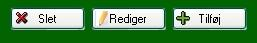
\includegraphics[width=0.99\textwidth]{Billeder/Gui/IkonKnapper.jpg}
  \caption{Ikoner p� knapper.\label{fig:IkonKnapper}}
\end{figure}

Som det kan ses p� figur \ref{fig:IkonKnapper} p� side \pageref{fig:IkonKnapper} har vi valgt at s�tte ikoner p� udvalgte knapper. M�let er, ved at bruge metaforer, at fremme brugerens intuitive forst�else af hvad knappen g�r. Problemet er i vores situation blot at vi ikke, igennem sessioner og samtaler med brugerne, i tilstr�kkelig grad har unders�gt om de ikoner vi har valgt har samme metaforiske betydning for brugerne som for os. Dette giver en hvis grad af usikkerhed omkring vores valg af metaforer. Vi skal ikke udvikle brugergr�nseflader ud fra vores egne opfattelser af metaforer, men inddrage brugeren og observere og bruge deres opfattelser. Under test i afsnittet \ref{TestSession} p� side \pageref{TestSession}, kan der l�ses om hvordan testen af vores applikation gik.

Vi har valgt at lave ikoner til 3 knapper, som alle g�r igen p� de sk�rmbilleder der er i systemet. Knappen 'Tilf�j', hvis form�l er at tilf�je en kunde eller et �konomisk forhold, er designet med et gr�nt plus-ikon. P� knapper, hvis funktion er at slette en kunde eller et �konomisk forhold, har et r�dt kryds som ikon.

\item Brugeren skal kunne forudse et programs opf�rsel, ved brug af sine erfaringer tilegnet fra andre programmer. Dette kaldes ``Princippet om konsistens p� platformniveau''. Konsistens er ikke kun vigtig i forbindelse med widgets, men ogs� i forbindelse med abstraktioner s�som musebev�gelser, menuplacering, ikoner og toolbarstil. Der er mange beslutninger vedr�rende brugergr�nseflader som er specifikke for den enkelte platform. Det er en god ide at finde og f�lge en god guide til design af brugergr�nseflader, rettet mod den platform der arbejdes med. Hvis man f�ler trang til at forbedre p� konventionerne, risikerer man at forstyrre brugernes vante opfattelser, hvilket netop er en af fordelene ved konventionerne; nemlig at sikre konsistens og standardisere design af brugergr�nseflader. Hvis man udvikler p� tv�rs af platforme er det vigtigt at holde konsistens med ``moderplatformen'', for ikke at opn� ukonsistens af applikationen p� tv�rs af platformene. Pointen er at brugeren skifter applikation p� samme platform, langt hyppigere end de bruger applikationen p� tv�rs af forskellige platforme \cite{MCToday}.

Som n�vnt tidligere udvikler vi i et udviklingsmilj� til Microsoft Windows, nemlig Visual Studio. Det er denne platform som vores brugere er vant til at bruge og vil komme til at bruge indenfor applikationens levetid. Ved at bruge Visual Studio f�r vi en masse ting omkring for eksempel printere og printdialoger til vores r�dighed. Dette betyder at vi med minimale anstrengelser kan lave Windowsspecifikke sk�rmdialoger. Hermed opn�r vi den fordel at vores brugere ikke skal s�tte sig ind flere nye ting end h�jst n�dvendigt.

\item Enhver brugeradvarsel og fejldialog, som opst�r p� grund af applikationen, skal ses som en chance for at forbedre brugergr�nsefladen. Gode brugergr�nseflader har sj�ldent brug for programadvarsler eller fejldialoger. Undtagelsen er selvf�lgelig hvor man ikke kan undlade at meddele om fejl, eksempelvis i forbindelse med hardwarefejl, diskfejl, tabt netforbindelse eller advarsler om at det skridt brugeren er ved at tage er irreversibelt og/eller kan medf�re fejl. Ellers ses fejldialoger i brugergr�nseflader som en designfejl. Det er bedre at forebygge, frem for at brokke sig over, at brugeren laver fejl. De hyppigste fejl kommer ofte fra ikke-korrekt formateret brugerinput i en uheldig r�kkef�lge. Dermed er det hensigtsm�ssigt at designe brugergr�nsefladen til at hj�lpe brugerne med at indtaste korrekt data. Hvis programmet kr�ver formaterede data (datoer, m�ntenheder med mere) s� kan man bruge 'begr�nsede' widgets til input, som p� hensigtsm�ssig m�de begr�nser brugerens inputmuligheder. Hvis et bestemt programtrin ikke kan udf�res ordentligt f�r brugeren fuldf�rer andre programtrin fuldst�ndigt, kan man s� vidt muligt skjule det afh�ngige trin, indtil alle afh�ngige forhold er fuldf�rte. For eksempel bruger de fleste brugergr�nseflademilj�er nedtonede widgets til at signalere at den p�g�ldene widget ikke kan v�lges p� nuv�rende tidspunkt. Man kan alts� bruge nedtonede widgets til at begr�nse brugerens handlinger til de tilladte. 

Her kan vi g�re to ting.

\begin{itemize}
\item Det skal synligg�res hvorn�r en knap er aktiv og hvorn�r den ikke er aktiv. Med andre ord, hvorn�r man kan trykke p� en knap og hvorn�r man ikke kan. Dette kan der l�ses mere om i afsnit \ref{kommentar_til_gui} p� side \pageref{kommentar_til_gui}. 
\item Det andet vi kan g�re er at sikre at felter som for eksempel telefon og personnummer kun kan tage imod tal. Ved at tjekke et felt hver gang noget bliver sat ind i det, kan vi sikre at der kun bliver tastet lovlige tegn. Skulle der eksempelvis blive tastet et bogstav i et felt der kun tager heltal, kan vi slettet dette bogstav. Fra brugerens synspunkt vil det se ud som om at programmet ikke reagerer p� andet end tal. Dette g�r at der ikke er behov for un�dige popup advarsler, hvilket er med til at sikre lovlige indtastninger. Punktet er dog blevet nedprioriteret i vores system, hvorfor vi ikke har fokuseret p� omr�det.
\end{itemize}

\item Vi skal str�be efter at f� vores applikation til at v�re selvforklarende. Gode applikationer har udf�rlige manualer og online hj�lpematerialer, der forklarer program features og hvordan de bruges til at l�se problemer i praksis. De bedste programmer er dem hvor brugeren sj�ldent har brug for at benytte manualen eller sl� op p� nettet. Forskellen mellem god og bedst afg�res ofte af hvor selvfoklarende applikationens brugergr�nseflade er. Lige fra valget af labels, skriftst�rrelser og fonttyper, til m�den hvorp� widgets arrangeres p� sk�rmen. Alle designbeslutninger der tr�ffes skal testes af brugere. M�let er at lave en brugergr�nseflade der ikke kr�ver un�dige forklaringer og dermed distraherer. Brugergr�nsefladen skal v�re selvforklarende for en bankr�dgiver, men ikke n�dvendigvis v�re det for en avisredakt�r.

Det vi har gjort i denne situation er at afholde prototypesessioner med brugerne for at finde ud af hvilke ord de s�tter p� deres arbejde og de processer de er involveret i. Hermed har brugerne i vores system bestemt navngivningen af indholdet i systemet, og dermed har de langt hen af vejen selv leveret teksten til de labels vi benytter. I et par tilf�lde har dette f�rt til at vi som udviklere er blevet lidt forvirrede omkring navngivningen. For eksempel hvorn�r det hedder et firma og hvorn�r det hedder et selskab. Det vigtigste her er dog brugbarheden af systemet og at kunden og brugerne er glade.

\item Vi skal undg� tvungen opf�rsel og adf�rd. 
Programmer der er pr�get af tvungen opf�rsel, tvinger brugeren til at udf�re opgaver i en bestemt r�kkef�lge eller p� andre m�der �ndrer p� brugerens forventede respons og adf�rd. Tvungen opf�rsel giver brugeren en generel fornemmelse af ubehag, fordi de begr�nser mere intuitive og naturlige handlinger. Brugt med omtanke kan tvungen opf�rsel dog have sine fordele. For eksempel i forbindelse med 'wizards', som gennem tvungen opf�rsel kan simplificere og guide en bruger gennem komplekse opgaver. Advarsler og fejlmeddelser er ligeledes ofte tvungne, hvilket tvinger brugeren til at tage stilling til et kritisk problem inden de kan vende tilbage til opgaven igen. Tvangen er i dette eksempel n�dvendig, men �del�gger ogs� brugerens koncentration og m�lrettede opf�rsel, og er derfor en grund til at undg� un�dvendige advarsler og fejlmeddelelser. 

De bedste tvungne opf�rsler er afd�mpede, men ikke skjulte. Eksempel: I et typisk tegneprogram giver valget af en widget en �ndret funktion, og giver derfor tvungen opf�rsel. Der er en tekstfelt-widget til at skrive tekst med, der er en pensel-widget til at male med, der er en figur-widget til at lave figurer med. Dette giver sj�ldent problemer, fordi den tvungne opf�rsel er bygget p� en analogi fra virkelighedens verden. % ved at v�lge tegneinstrumenter er der begr�nsninger i farven, teksturen og linietykkelsen der kommer p� vores papir. 
Gode brugergr�nseflader �ndrer musemark�ren for at give yderligere visuel feedback n�r et valg er truffet. S� hvis applikationen absolut kr�ver tvungen opf�rsel, skal man s�rge for at binde den til en st�rk metafor og giv brugeren visuel feedback, hvormed det kan forl�be mere naturligt og ligefremt. 

Vi g�r, til dels, brug af tvungen opf�rsel, n�r brugeren eksempelvis skal oprette en indt�gt. F�rst v�lger man hvilken kunde indt�gten skal tilh�re, trykker tilf�j, v�lger indt�gten, indtaster de relevante data og trykker tilf�j. P� den anden side har vi en navigationsbar som g�r at brugeren frit kan springe mellem de forskellige sk�rme, som p� den m�de sikrer at systemet har en vis fleksibilitet n�r det kommer til forskellige arbejdsformer.

\item Brugergr�nsefladen skal designes s� brugeren kan udf�re sine opgaver uden at ligge synderligt m�rke til brugergr�nsefladen i sig selv. Dette kunne kaldes 'Princippet om gennemsigtighed'. Gr�nseflade-gennemsigtighed sker n�r brugerens opm�rksomhed rettes v�k fra selve gr�nsefladen og naturligt rettes mod opgaven. Dette opn�s gennem flere faktorer, inklusivt et sk�rmlayout hvor b�de v�rkt�j og information er hvor brugeren forventer de skal v�re, hvor ikoner og labels giver mening for brugeren og hvor de brugte metaforer er let genkendelige og dermed lette at l�re, huske og udf�re. At v�lge gode metaforer og f�lge ovenn�vnte principper er en vigtig start, men den mest direkte m�de at sikre en gennemsigtig brugergr�nseflade er ved at udf�re brugertests gennem hele programmets udviklingsforl�b.

Dette er en af de ting vi kunne have gjort anderledes. Vi har brugt tid og kr�fter p� at f� information omkring hvad systemet skal kunne, men vi har ikke brugt tid nok p� at unders�ge hvor p� sk�rmen brugeren helst ser knapper og elementer placeret. Brugerne har haft mulighed for dette under prototypesessionerne, men der har ikke v�ret fokuseret p� det.

Da EIK Banks medarbejdere fra private banking er vant til regnskab og regenark, kunne det v�re en fordel hvis vi fik medbragt elementer fra regneark. Dette kunne v�re datagrids i stedet for tekstfelter, i forbindelse med indtastning. Generelt er der, hos afdelingens medarbejdere, en fork�rlighed for at f� stillet ting op i r�kker og kolonner.
\end{enumerate}

\subsection{Menneskelig opfattelse}
N�r mennesker skal opfatte mange elementer p� en gang har vi en tendens, nogle siger at det er et overlevelsesinstinkt, til at gruppere og forudindtage synsindtryk. Ser vi en del af noget, er vi meget hurtige til ubevidst at bygge videre p� dette synsindtryk. Dette g�r vi for hurtigt at kunne reagere p� en fare.

N�r det kommer til at t�lle mange elementer g�r vi brug af forskellige teknikker til at simplificere opgaven. En af disse teknikker g�r ud p� at gruppere elementerne. Skal vi for eksempel t�lle prikker p� et stykke papir, kan vi hj�lpe os selv ved at s�tte ring omkring fem t�tliggende elementer. Derefter kan man s� t�lle ringene, gange med 5 og l�gge en eventuel rest til. Der er ogs� forskellige teknikker til at gruppere elementer og disse teknikker kommer vi indvp� i afsnittet om Gestaltlovene \ref{Gestaltlovene} p� side \pageref{Gestaltlovene}.

Et andet omr�de hvor vi som mennesker laver opdelinger, er n�r husker tal. For eksempel kan det v�re sv�rt at huske et telefonnummer. Dette kan g�res nemmere ved at dele telefonnummeret op i mindre dele. For eksempel 12 34 56 78 eller 123 456 78 eller 12 345 678, hvor de to sidste opdelinger ikke er s� gode, da vores telefonnumre ikke er delelige med 3. Tricket best�r i at gruppere p� en s�dan m�de at grupperne er mindst mulige, samtidigt med at der er s� f� grupper som muligt. 
Disse to krav er i modstrid med hinanden og det er et kompromis mellem disse der f�r metoden til at virke. Et andet eksempel p� hvor vi deler en opgave op er regnestykker. For eksempel er $14*5=70$, men dette er m�ske ikke lige til at se. Deler vi derimod opgaven op p� en anden m�de bliver det m�ske lidt nemmere. For eksempel ved at sige $10*5+4*5=50+4*5=50+20=70$ eller ved at indse at 14 er en mindre end 15 og s� sige $5*15-5*1=75-5*1=70$.

\subsection{Gestaltlovene}\label{Gestaltlovene}
\subsubsection{Generel teori omkring gestalt}
Gestaltlovene handler om opfattelse af helheder i et billede. Gestalt er en fri overs�ttelse af det tyske ord gestellt, der betyder 'opstilt'. Der er mange gestaltlove, der tilsammen beskriver hvordan man kan designe indholdet p� sk�rmbilleder til at h�nge sammen. Man kan sige at et godt design hj�lper brugeren ved ikke visuelt at distrahere denne fra den egentlige arbejdsopgave. 
De regler der er relevante i forhold til vores projekt beskrives som f�lger:

\begin{itemize}
\item \textbf{Loven om n�rhed:}
Det er vigtigt at elementer der har relation til hinanden, er placeret t�t ved hinanden og dermed opfattes som sammenh�ngende. Man kan alts� danne en gruppering af elementer, ved at placere dem n�r hinanden. For eksempel kan en 'label' (l�s: tekst), der er placeret for langt fra dens tilh�rende 'textbox' (l�s: tekstfelt), resultere i at de to elementer ikke opfattes som sammenh�ngende. Man risikerer yderligere at den p�g�ldende 'label' ligger for t�t p� et andet element som den ikke har nogen relation til. Dermed kan deciderede misforst�elser opst�, hvor brugeren tror at der skal tastes i et andet felt end det tilt�nkte. Loven bruges hermed til at vise hvilke elementer der h�rer sammen. Dette kan opn�s ved et samspil mellem velafstemte mellemrum og brug af r�kker og kolonner.

\item \textbf{Loven om lukkethed:}
For at tydeligg�re sammenh�ngen af et sk�rmbilledes elementer, kan man lukke grupper af elementer inde i en ramme, en s�kaldt 'groupbox' (l�s: ramme). En fornuftig brug af rammer, kan v�re med til at h�jne visualiseringen af sammenh�ngende elementer. Med en fornuftig brug menes at det ikke nytter noget at bruge for mange rammer p� samme sk�rmbillede, hvilket resulterer i et rodet layout.

\item \textbf{Loven om lighed:}
Man grupperer normalt elementer efter hvor meget de ligner hinanden. Dette betyder at elementer der ligner hinanden er placeret t�t op af hinanden, for at tydeligg�re deres betydning. Rent visuelt kan dette eksempelvis opn�s ved brug af fonte, font st�rrelser og farver. Et eksempel p� dette kan v�re grupperingen af knapperne i v�rkt�jslinien i Word, hvor sidestilnings-knapperne ligner hinanden og dermed grupperes sammen. 

\item \textbf{Loven om symmetri:}
Denne regel omhandler brugen af linier og symmetri i sk�rmbilledet. Dette betyder at billedets elementer helst skal flugte med og v�re visuelt knyttet med hinanden, for at skabe et indtryk af balance og helhed. Hvis der er en tydelig asymmetri i sk�rmbilledet, vil dette forvirre og distrahere brugeren.

\item \textbf{Loven om kontinuitet:}
De indirekte linier mellem sk�rmens elementer, som er baseret p� kontinuitet, giver en �get opfattelse af sammenh�ng og gruppering. Mennesket har tendes til at f�lge linier, eksempelvis pile der peger i en retning.
\end{itemize}

Gestaltlovene omfatter generelle elementer i brugergr�nseflade s� som menuer, knapper og ikoner, grafer, tabeller, tekst. De forskellige love skal ikke opfattes som s�rskilte og isolerede fra hinanden, men n�rmere som sammenh�ngende. Sammen giver de en h�j grad af logisk visualisering. Det vil sige at gestaltteorien f�lger princippet om at af helheden er st�rre end summen af delene, se kilde \cite{Gestalt}.

\subsubsection{Vores brug af Gestaltlovene}
Vi har i vores system brugt de gestaltlove som var relevante for vores system. Nedenfor kan ses eksempler p� hvor vi har fundet anvendelse for af forskellige love.
\begin{enumerate}
\item N�rhed: Navigeringsknap-menuen.

\item Lukkethed: Groupboxes.

\item Lighed: Indtastnings felter til kunde oplysninger.

\item Symmetri: Navigeringsknap-menuen.

\item Kontinuitet: Navigeringsknap-menuen.
\end{enumerate}

Se figur \ref{fig:GuiGestalt} p� side \pageref{fig:GuiGestalt}.\\
\begin{figure}
	\centering
		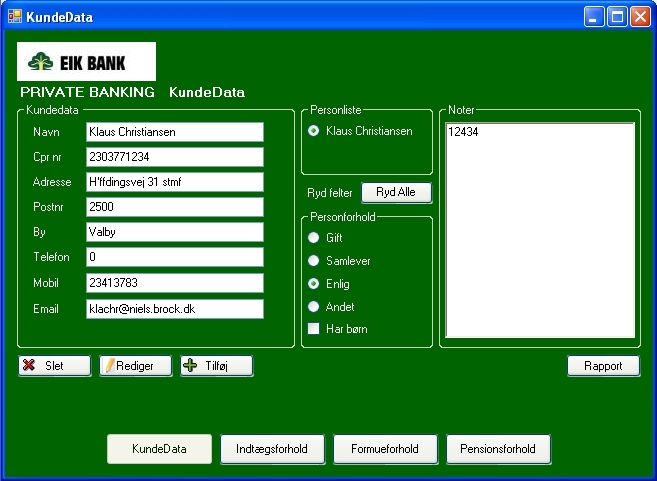
\includegraphics[width=1.00\textwidth]{Billeder/Gui/GuiGestalt.jpg}
	\caption{Gestalt i vores gui.\label{fig:GuiGestalt}}
\end{figure}


\subsubsection{Fremtoning}
\textbf{Ny session}\\
F�rst n�r der skrives i textbox $\Rightarrow$ OK knap enables.\\

\textbf{Indt�gtsforhold}\\
N�r ingen person er valgt $\Rightarrow$ 'Slet', 'Rediger' og 'Tilf�j' gr�tones og disables.\\
N�r en person v�lges $\Rightarrow$ 'Tilf�j' optones og enables.\\
N�r en indt�gt v�lges $\Rightarrow$ 'Slet' og 'Rediger' optones og enables.\\
\\
\textbf{Formueforhold}\\
N�r ingen person er valgt $\Rightarrow$ 'Slet', 'Rediger' og 'Tilf�j' gr�tones for b�de 'Aktiver' og 'Passiver'.\\
N�r en person v�lges $\Rightarrow$ 'Tilf�j' optones og enables for b�de 'aktiver' og 'passiver'.\\
N�r et aktiv v�lges $\Rightarrow$ 'Slet' og 'Rediger' optones og enables.\\
N�r et passiv v�lges $\Rightarrow$ 'Slet' og 'Rediger' optones og enables.\\
\\
\textbf{Pensionsforhold}\\
N�r ingen person er valgt $\Rightarrow$ 'Slet', 'Rediger' og  'Tilf�j' gr�tones og disables.\\
N�r en person v�lges $\Rightarrow$ 'Tilf�j' optones og enables.\\
N�r en pension v�lges $\Rightarrow$ 'Slet' og 'Rediger' optones og enables.\\
\\
\textbf{Tidligere session, Sessionsvalg}\\
N�r Tidligere sessioner er valgt og ingen session er valgt $\Rightarrow$ 'OK' knappen gr�tones og disbles.\\
N�r man vender tilbage til sessionsvalgsform $\Rightarrow$ nusltil alle felter.\\
N�r man skifter fra ny session (hvor OK enables) til tidl session skal OK $\Rightarrow$ disables.\\

\textbf{Kundedata}\\
Ingen kunder i sessionen $\Rightarrow$ radiobuttons visiblity = false; (g�lder ved f�rste load af formen).\\
N�r man trykker p� 'RydAlle' knap skal information i alle felter slettes, og radioknapperne til personerne v�re unchecked.\\
N�r ingen kunde er valgt $\Rightarrow$ 'Slet' og 'Rediger' gr�tones og disables. Se figur \ref{fig:KundeData1} p� side \pageref{fig:KundeData1}.\\
\begin{figure}
	\centering
		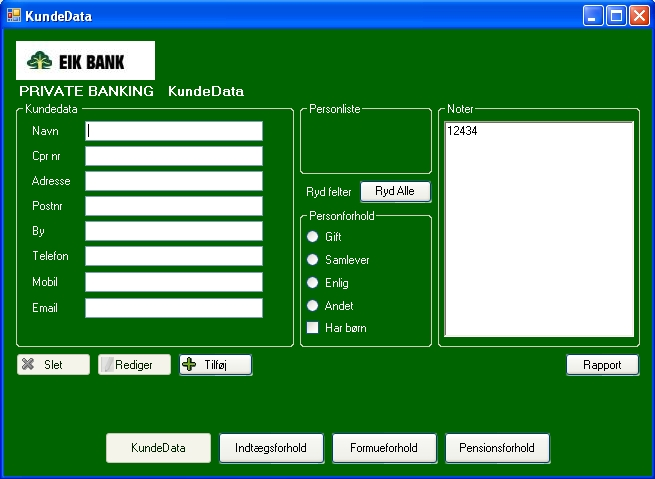
\includegraphics[width=1.00\textwidth]{Billeder/Gui/KundeData1.jpg}
	\caption{KundeData: ingen kunde valgt.\label{fig:KundeData1}}
\end{figure}
N�r en person v�lges p� personlisten $\Rightarrow$ 'Slet' og 'Rediger' optones og enables. Se figur \ref{fig:KundeData2} p� side \pageref{fig:KundeData2}.\\
\begin{figure}
	\centering
		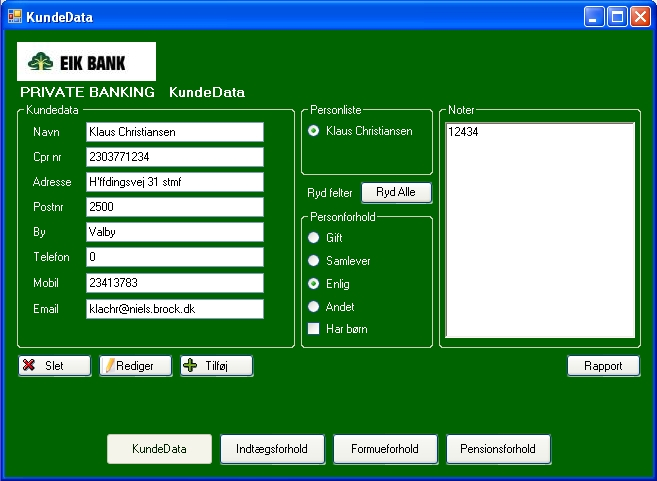
\includegraphics[width=1.00\textwidth]{Billeder/Gui/KundeData2.jpg}
	\caption{KundeData: en kunde er valgt.\label{fig:KundeData2}}
\end{figure}
N�r der er 2 person i forholdet $\Rightarrow$ 'Tilf�j' gr�tones og disables.\\

\textbf{Indt�gtsforhold}\\
N�r ingen person er valgt $\Rightarrow$ 'Slet', 'Rediger' og 'Tilf�j' gr�tones og disables.\\
N�r en person v�lges $\Rightarrow$ 'Tilf�j' optones og enables.\\
N�r en indt�gt v�lges $\Rightarrow$ 'Slet' og 'Rediger' optones og enables.\\

\textbf{Formueforhold}\\
N�r ingen person er valgt $\Rightarrow$ 'Slet', 'Rediger' og 'Tilf�j' gr�tones for b�de 'Aktiver' og 'Passiver'.\\
N�r en person v�lges $\Rightarrow$ 'Tilf�j' optones og enables for b�de 'aktiver' og 'passiver'.\\
N�r et aktiv v�lges $\Rightarrow$ 'Slet' og 'Rediger' optones og enables.\\
N�r et passiv v�lges  $\Rightarrow$ 'Slet' og 'Rediger' optones og enables.\\

\textbf{Pensionsforhold}\\
N�r ingen person er valgt $\Rightarrow$ 'Slet', 'Rediger' og 'Tilf�j' gr�tones og disables.\\
N�r en person v�lges $\Rightarrow$ 'Tilf�j' optones og enables.\\
N�r en pension v�lges  $\Rightarrow$ 'Slet' og 'Rediger' optones og enables.\\

\subsubsection{Kommentar til brugergr�nsefladen\label{kommentar_til_gui}}
Noget af det f�rste der falder os, som udviklere, i �jnene er hvor sv�rt det er at se forskel p� om en knap er klikbar eller ikke klikbar. Grunden til dette skal finde i farvevalget, hvor baggrunden er m�rke gr�n og knapperne er gr�. Et andet problem er at vi har ladet Visual Studio tage sig af forskellene mellem en klikbar og en ikke klikbar knap. En ting vi kunne havde gjort for at forst�rke budskabet om hvorvidt en knap er klikbar eller ej, er at vi kunne havde gjort teksten p� den p�g�ldende knap mindre tydelig. Dette kunne vi g�re ved at v�lge en tekstfarve som ligger t�t p� knappens baggrundsfarve. Samtidig kunne vi havde valgt farverne p� knapper s�dan at de n�sten gik i et med sk�rmens baggrundsfarve. Dette ser vi dog ikke som v�rende n�dvendigt med de knapper som har ikoner. Disse ikoner har vi i to versioner, en med farve til n�r knappen er klikbar og en uden farver til n�r knapperne ikke er klikbare.

\newpage
\section{Design patterns\label{design_pattern}}

Da der foreligger et krav om at vores system skal v�re modul�rt og udvidelsesvenligt, er det n�rliggende at se p� om vi kan indkorporere design patterns i systemarkitekturen. Design patterns g�r ud p� at genkende m�nstre i udviklingsfasen og s� lave en l�sning som er s� generel at den kan genbruges n�ste gang vi st�der p� dette m�nster. 

Der findes mange forskellige design patterns som tager sig af forskellige problemomr�der, 
p� forskellige m�der. Man kan bruge disse forskellige m�der at tackle problemer og/eller opgaver p�, til at kategorisere design patterns i 3 kategorier. De konstruerende, de strukturelle og de handlingsorienterede patterns.

De konstruerende patterns omhandler hvordan man opretter objekter. De strukturelle patterns tager sig af arkitekturen i designet. De handlende patterns fokuserer p� hvordan man behandler objekter og hvordan man designer fremtidssikrede applikationer med videre.

Design patterns giver flere fordele:
\begin{itemize}
\item Genbrugbarhed af gode l�sninger.
\item Skaber f�lles forst�else og kommunikation mellem udviklere.
\item At t�nke probleml�sning p� et h�jere og mere abstrakt plan.
\item Til at beslutte om vi har det rigtige design eller blot et der virker.
\item G�r koden nemmere at �ndre.
\item G�r designet mere modul�rt.
\item G�r koden mere flexibel.
\item G�r kode og design mere elegant.
\end{itemize}

\subsection{Model View Controller\label{MVC}}
Vi vil i dette projekt kigge n�rmere p� det design pattern der hedder MVC\footnote{Model View Controller}. Form�let med dette pattern er at dele et systems ansvarsomr�der op i tre dele, p� en s�dan m�de at de tre dele bliver uafh�ngige af hinanden. Det er her, n�r det kommer til udvidelsesvenlighed, at MVC bliver brugbart. Det er modellagets ansvar at styre behandling af data, databaseadgang og forretningslogik. Det data der bliver sendt fra modellaget skal v�re brugergr�nseflade uafh�ngigt, hvorved s� mange forskellige views som mulig kan bruge modellen. Kontrollaget har ansvaret for at reagere p� forandringer i brugergr�nsefladen (input fra brugeren). Kontrollaget giver modellaget besked om at den skal �ndre sig og giver besked til view om at der er sket �ndringer i modellen, s�dan at view skal opdatere sig. Det er viewlagets ansvar at pr�sentere data for brugeren, det vil sige at view st�r for alt hvad der har at g�re med 'look and feel'. Med 'look and feel' menes at det er view der st�r for at formatere data inden det pr�senteres for brugeren.

Der er to m�der at anskue MVC p�, hvor den ene er en aktiv model og den anden er en passiv model. I den passive model �ndrer modellaget sig kun n�r kontrollaget giver besked om det. Dette medf�rer at modellaget har lav kobling med view og kontrol, hvilket betyder at modellaget ikke ved at de eksisterer. I den aktive model er der andre end view og kontrol som kan �ndre modellaget, dette kunne v�re andre modellag, hvilket g�r at modellaget bliver n�dt til at give bedsked til view om at den har �ndret sig. I dette tilf�lde er det n�rliggende at g�re brug af at et andet design pattern, nemlig Observer, ogs� kaldet Subscriber/Publisher. Ideen er at view tilmelder sig de modeller de gerne vil have besked fra n�r der sker �ndringer i dem. Modellaget giver dermed besked til alle p� listen og viewlaget kan nu hente de nye data. 

Hele form�let med design patterns er at generalisere sine l�sninger og derigennem at kunne genbruge sin kode og de erfaringer man har med at bygge arkitektureren. Der er ingen grund til at skulle opfinde den dybe tallerken for hver gang man skal strukturere et system. 

Det vi vil opn� med MVC er at g�re vores system udvidelsesvenligt. Det smarte er at vi kan �ndre forretningslogikken uden at skulle �ndre i kontrol og viewlaget.

Et eksempel p� brugen af MVC.

\lstset{language=[Sharp]C, % fort�ller hvilket sprog koden er skrevet i [dialekt].
  basicstyle=\small, breaklines=true}

\begin{lstlisting}
public partial class KundeData : Form
{
  KundeKontrol kundeKontrol = new KundeKontrol();
  Session session = new Session();

  private void rdoPerson1_CheckedChanged(object sender, EventArgs e)
  {
     kundeKontrol.getEvent(sender);
  }

  public void VisKunde(Kunde k)
  {
    Kunde k = session.GetKundeKontainer().GetKunde(0);
    this.txtNavn.Text = k.Navn;
    this.txtCpr.Text = "" + k.CPR;
    this.txtAdresse.Text = k.Adresse;
    this.txtPostnr.Text = "" + k.PostNr;
    this.txtBy.Text = session.GetBy(k.PostNr);
    this.txtTelefon.Text = "" + k.Telefon;
    this.txtMobil.Text = "" + k.Mobil;
    this.txtEmail.Text = k.Email;
    this.chkHarBoern.Checked = k.HarBoern;

    if (k.CivilStatus == 1)
      this.rdoStatusGift.Checked = true;
    else if (k.CivilStatus == 2)
      this.rdoStatusSamlever.Checked = true;
    else if (k.CivilStatus == 3)
      this.rdoStatusEnlig.Checked = true;
    else
      this.rdoStatusAndet.Checked = true;
  }
}

public class KundeKontrol
{
  public void getEvent(object sender)
  {
    if (SenderRdo.Name == "rdoPerson1" && kundeForm.rdoPerson1.Checked)
    {
      if (session.GetKundeKontainer().GetAntalKunder() >= 1)
      {
        kundeForm.VisKunde(k);
      }
    }
  }
}
\end{lstlisting}

\begin{figure}
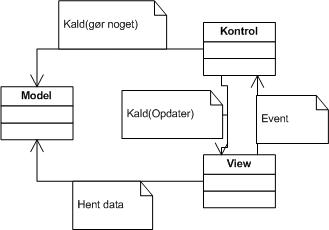
\includegraphics{Billeder/MVC.jpg}
\caption{MVC diagram.}
\end{figure}

N�r brugeren trykker p� en knap p� sk�rmen, sender view et eventobjekt videre til kontrollaget, som f�r modellaget til at udf�re forretningslogikken. N�r modellaget s� er f�rdig giver kontrol laget besked til view om at den skal opdatere sine data.

Et af de problemer vi har haft med MVC, g�r ud p� at placere ansvar mellem kontrollaget og viewlaget. Det er som sagt view der st�r for at formatere og pr�sentere data, og det er kontrollaget der bestemmer hvad der skal vises n�r det kommer til knapper og andre elementer p� sk�rmen. Man kan sige at view bestemmer hvordan data vises og kontrollaget bestemmer hvorn�r data vises og hvilke data der vises. Denne balance kan dog gradb�jes og vi oplevede situationer hvor man kunne diskutere hvor det er mest hensigtsm�ssigt at placere disse ansvarsomr�der, alt efter hvilken kode vi stod med. 

Det er ogs� kontrollagets ansvar at fort�lle modellaget at den skal �ndre sig, men det kan til tider v�re sv�rt udelukkende at holde sig til brugen af kontrol laget. Dette g�lder specielt n�r view skal pr�sentere noget som er dynamisk og et element p� sk�rmen har betydninger for et andet element. Det betyder at view skal bruge data, som view kun kan f� ved at bede modellaget om at lave beregninger. Da vi startede med at kode MVC var vores intention at view kun skulle tilg� modellen med 'get' metoder. Vi har s� senere v�re n�d til at �ndre denne opfattelse, i retning af at view ogs� m� bede modellen om at lave beregninger. Det er dog stadigt kun kontrol som m� bede modellen om at �ndre sig. Hele denne diskussion bunder i disciplin, og jo mere disciplineret og konsekvent vi koder systemet des nemmere bliver koden at gennemskue, b�de for os og for andre udviklere.

Til emnet om design patterns og specielt til MVC har vi gjort brug af f�lgende kilder: \cite{msdnMVC}, \cite{MVC_in_.NET} og \cite{Smalltalk-80}.

\subsection{Singleton\label{singleton}}
Singleton er et andet design pattern som vi, i modularitetens navn, kan g�re brug af. Ideen med dette pattern er at uanset hvor mange gange man instantierer et objekt, som er kodet som en singleton, s� bliver der i memory kun oprettet et objekt ad gangen. Database-tilgangen er en oplagt klasse at implementere som singelton. En fordel ved dette pattern er at der ikke bliver brugt n�r s� meget tid p� at oprette objekter p� heapen.\\

Det kunne se s�dan her ud.
\lstset{language=[Sharp]C, % fort�ller hvilket sprog koden er skrevet i [dialekt].
  basicstyle=\small, breaklines=true}

\begin{lstlisting}
Class DBAccess{        
  private static DBAccess dbInstance;
  public static DBAccess GetDBInstance()
  {
    if (dbInstance == null)
      dbInstance = new DBAccess();
    return dbInstance;
  }

  private DBAccess()
  {
    string stiTilDB = "C:/Documents and Settings/ideas/Skrivebord/HovedOpgave/Test/Accesstestdb/testdb.mdb";
    string ConnString = "Provider=Microsoft.Jet.OLEDB.4.0;Data Source=" + stiTilDB;
    myConnection = new OleDbConnection(ConnString);
    myConnection.Open();
  }
}

public static void main(String[] args)
{
  DBAccess.getDBInstance().Udf�r et eller andet();
}
\end{lstlisting}

Ved at g�re konstrukt�ren privat forhindrer vi, at der kan oprettes flere objekter af typen DBAccess. Dermed er man tvunget til at bruge metoden GetDBInstance som, via if-s�tningen, sikrer at der til enhver tid kun eksisterer �t DBAccess objekt.

%Kilder: http://msdn.microsoft.com/library/en-us/dnpatterns/desmvc.aspx
%http://www.marcclifton.com/Articles/DeclarativeProgramming/MVCPatternandDataBinding/tabid/96/Default.aspx
%http://www.c-sharpcorner.com/Code/2003/Feb/MVCDesign.asp
%http://st-www.cs.uiuc.edu/users/smarch/st-docs/mvc.html

\chapter{Test}

En del af opgaven i forbindelse med udviklingen af et IT-system handler om at sikre kvaliteten af det udviklede produkt. Med kvalitet t�nkes der p� flere aspekter. Et aspekt er for eksempel 
sikkerheden i systemet, hvilket ikke er uv�sentlig i vores projektsammenh�ng. Et andet aspekt 
er rigtigheden af de beregninger systemet laver og om de udviklede algoritmer rent faktisk 
udf�rer den opgave de er konstueret til at udf�re. Man kan ligeledes unders�ge og teste om 
systemet opfylder den �nskede grad af brugervenlighed og fleksibilitet, som dog er lidt bl�dere 
emner der kan v�re sv�re at give et konkret svar p�. Hvis man ikke unders�ger disse, og andre, 
kvalitetsm�ssige aspekter under udviklingsfasen, risikerer man at systemet i sidste ende ikke 
er brugbart. Denne kvalitetssikring opn�s prim�rt gennem forskellige former for tests af systemet, b�de af systemet som helhed og af de involverede delsystemer.

For at kunne teste et specifikt omr�de af et system, er det n�dvendigt at planl�gge testsituationen og g�re sig klart hvad det er man vil teste og hvordan man vil teste det. Det giver typisk mest mening at teste b�de indenfor og udenfor normalomr�det af det data systemet kan repr�sentere. Hvis en funktion for eksempel ikke skal kunne kan behandle negative heltal, er det hensigtsm�ssigt at teste om den s� kan h�ndtere positive heltal, men bestemt ogs� at teste p� hvad der sker hvis funktionen mod forventning skulle modtage et negativt heltal. Der skal, s� vidt muligt, tages h�jde for uventede situationer og fejlbehandling af disse, for at undg� at systemet i yderste konsekvens fejler og/eller g�r ned.

\section{Testmodeller}
Der ligger meget teori og forberedelse til grund for at kunne udf�re tests. Da testemnerne kan v�re ganske forskellige, er det n�dvendigt at have forskellige testmodeller til at kunne d�kke de forskellige test forhold.

Whitebox er en testmodel der bruges til at teste enkelte funktioner i systemet. Man dykker alts� ned i systemets kode og udv�lger typisk dele af denne som testmateriale. Kriterierne for om en funktion best�r en whitebox test ligger i de pre- og postconditions der er opstillet for funktionen. Whitebox tester alts� om pre- og postconditions bliver overholdt.

Blackbox ser, som navnet antyder, systemet som en lukket enhed der skal testes, uden kendskab til hvordan systemets interne dele fungerer. Denne testmodel giver input til et givent system og tager derefter det output systemet leverer, som resultat. Med 'et system' menes ikke n�dvendigvis en hel og f�rdig applikation, men kan ogs� v�re et delsystem.



\section{Testsession\label{TestSession}}
Test af applikationen handler ikke kun om test af koden, men ogs� om test af andre omr�der som for eksempel brugergr�nseflade. Efter at applikationen er kodet, b�r den testes i dens tilsigtede milj�, for at se om den lever op til de krav vi har formuleret i samarbejde med EIK Bank. Kravene er m�lbare og best�r i, at den tid indtastningen af en typisk kundes stamdata tager, skal nedbringes ved hj�lp af vores applikation. P� nuv�rende tidspunkt og med nuv�rende arbejdsgang ligger indtastningstiden p� ca. 30-60 min. for en gennemsnitskundes datas�t. Kravet er formuleret s�dan, at dette skal forbedres efter 5-10 fors�gsrunder med applikationen, ned til i omegnen af 15-30 min, se tabel \ref{Kravliste} p� side \pageref{Kravliste}.

\subsection{Test af applikationen}
For at teste vores applikation vil vi afholde en testsession. Der er dog nogen ting vi b�r overveje og planl�gge inden vi afholder denne. Vi b�r overveje valg af testsubjekter, hvordan testen udf�res og hvilken hypotese som skal testes af. Hypotesen bliver formuleret p� tilsvarende m�de som ovenfor. 
\begin{itemize}
\item Hypotese: Vores applikation kan hj�lpe til at bringe indtastningstiden ned til i omegnen af 15-30 min.
\end{itemize}
%Hvordan ser den bedst mulige testsession ud?

\subsubsection{Den ideelle test}
Milj�et der testes i b�r v�re s� t�t p� applikationens tilsigtede milj� som muligt. Dette inkluderer selvf�lgelig brugerne, som b�r have de samme f�rdigheder og vidensniveau, som de brugere, der skal arbejde med applikationen i fremtiden. I en ideel testsession vil vi have, de anbefalede, minimum 10 testpersoner, se kilde\cite{HCI}. Vi kalder dem fremover testbrugere, istedet for testpersoner, da det er applikationen og ikke selve personerne der skal testes.
 
Vi vil foretage opm�linger af, hvor langt tid det tager at indtaste en kundes data, med r�dgivernes nuv�rende arbejdsgang. Dette vil foreg� i deres vante arbejdsomgivelser. En gruppe p� minimum 10 testbrugere indtaster datas�t af gennemsnitsst�rrelse p� vores system. Efter 5 til 10 fors�g findes den bedste tid, og s� har vi et m�l for tiden det tager at indtaste datas�ttet. En sammenligning mellem tiderne for det gamle og vores nye system vil nu v�re muligt. Det samme vil en vurdering af effekten af det nye system. 


\subsubsection{Vores testsession}
Hvordan blev vores testsession s� egentlig afholdt? P� trods af at vi er s� heldige at have tilgang til de selvsamme brugere, som rent faktisk kommer til at benytte systemet i fremtiden, s� har vi kun 2 testbrugere og ikke de anbefalede minimum 10. Dette kommer vores testresultater naturligvis til at lide under rent statistisk set. P� dagen for testsessionen viser det sig uheldigvis, at antallet af testbrugere er reduceret til �n, p� grund af sygdom.

Vi afsatte en time til testsessionen, fordelt p� � time til selve udf�rslen af testen og � time til uformel snak om sessionen. Vi fordelte roller mellem os. Der var en til at byde velkommen og efterf�lgende v�re observat�r, endnu en observat�r og en facilitator. Vi benyttede et tidligere udleveret datas�t, som testbrugeren skulle k�re igennem. Dette datas�t bestod af materiale fra en rigtig kundesag. Testbrugeren blev stillet to scenarier. F�rst skulle testbrugeren finde kundens stamdata i datas�ttet og indtaste dem, dern�st skulle indt�gtsforholdene findes og indtastes. Herefter stillede vi en h�ndfuld improviserede till�gssp�rgsm�l, hvor testbrugeren blev bedt om at redigere og slette henholdsvis en indt�gt og en person, for at komme rundt i de sidste dele af systemet. I samtalen med EIK Bank r�dgiveren bagefter, ville vi fokusere p� systemets brugervenlighed og effektivitet, og tage noter imens.


\subsection{Resultat af testsessionen}
Sessionen forl�b fint og varede pr�cist en time som planlagt. Tidsm�ssigt tog det testpersonen 11 minutter og 24 sekunder at indtaste henholdsvis kundedata, indt�gtsforhold og det tog yderligere 3 minutter og 31 sekunder komme igennem rediger og slet funktionerne. 

Navigeringen rundt mellem de forskellige forme gik faktisk ret godt. Der var dog lidt forvirring omkring 'tilf�j' knappen. Under oprettelsen af en kunde gik det fint nok med at trykke p� 'tilf�j' knappen, men da der skulle oprettes en indt�gt, gik der l�ngere tid inden testbrugeren fandt ud af, at man skulle markere en kunde, inden man kunne trykke p� 'tilf�j' knappen. Herefter var der skabt forst�else for, at en kunde skulle markeres f�r der kunne indtastes data. 'Rediger' og 'slet' indt�gter virkede ikke helt intuitivt for testbrugeren og kr�vede lidt hj�lp at komme igennem. Det skal s� n�vnes at det var f�rste gang testbrugeren s� og anvendte systemet, udover at have set prototyperne. Testbrugeren fik ikke tid til f�rst at l�re systemet at kende. Sessionen begyndte med det samme.

Der var ogs� lidt forvirring i begyndelsen omkring, at en kunde h�rer sammen med en session. Alts� at der ikke kan eksistere en kunde uden at der eksisterer en session. Dette kunne der sandsynligvis rettes op p� ved at kalde en 'session' for en 'sag' i stedet for, har vi erfaret efterf�lgende. Bortset fra ovenn�vnte problemer navigerede testbrugeren ret godt rundt i programmet.

Under samtalen bagefter kom vi lidt ind p� de tidsm�ssige aspekter i systemet, brugergr�nsefladen og systemet generelt. Vi fandt frem til en hel del forslag til hvordan applikationen kan forbedres. B�de nogle vi var klar over og nogle der var nye. Her er noget af det vi fandt frem til:

Kundedata
\begin{itemize}
\item P� nuv�rende tidspunkt stiller programmet krav om at der under oprettelsen af en kunde skal indtastes f�lgende stamdata: 'CPR nummer', 'postnummer', 'mobilnummer' og 'telefonnummer', mens 'Navn', 'adresse' og 'email' kan udelades. For fleksibilitetens skyld vil det v�re bedre hvis det kun var 'Navn' og 'CPR nummer' der var n�dvendige at indtaste.
\item I den situation hvor der skal tilf�jes en person nr. 2, burde systemet v�re skruet s�dan sammen, at efter der er blevet trykket p� tilf�j, skulle alt information i textfelterne der er indtastet bevares. Kun 'CPR nummer' og 'Navn' skal ryddes.
\end{itemize}


Indt�gtsforhold
\begin{itemize}
\item Der �nskes helt overordnet en opdeling af ansvaret mellem popup�en og indt�gtsformen, p� en s�dan m�de, at indt�gtsformen giver overblikket og popup�en giver detaljerne.
\item For testbrugeren virkede det mere logisk at have knapperne til 'tilf�j', 'slet' og 'rediger' p� popup-formen.
\item Sum p� popup-formen. S�ledes at der er en samlet sum for den enkelte kategori, f.eks. aktier.
\item Totalsum p� hovedformen. Totalsum for samtlige kategorier p� formen, alts� alle indt�gter.
\item N�r der tilf�jes en ny indt�gt skal den ikke inds�ttes nederst i treeview'et p� indt�gtsformen, men f�lge samme r�kkef�lge af indt�gter som p� popup'en. Treeview b�r alts� v�re sorteret.
\item P� popup'en �nskes det, at alle posteringerne under den enkelte kategori skal listes p� �n gang og at de skal listes i r�kker og kolonner.
\item Kundens navn p� popup sk�rmen vil m�ske v�re en god ide.
\end{itemize}


Generelt
\begin{itemize}
\item Fortrydknap: Testbrugeren efterspurgte en 'fortrydknap', som han kendte fra andre programmer. Han synes dog ikke problemet er s� stort, da der ikke er nogen reel risiko for at miste data. Al informationen der skal indtastes, ligger alligevel i kundens datas�t og kan indtastes igen.
\item En advarsel n�r brugeren v�lger 'slet', som beder om en bekr�ftigelse af sletningen.
\item Tusindtalsseperatorer for at tydeligg�re bel�benes st�rrelser.
\end{itemize}


Vi fik ogs� input til vores grafiske brugergr�nseflade. Testbrugeren tillagde ikke ikonerne p� 'tilf�j', 'slet' og 'rediger' knapperne nogen betydning. Plustegnet p� 'tilf�j' knappen og krydset p� 'slet' knappen gav ikke nogen associationer i retning af at slette og tilf�je. Blyanten p� 'rediger' knappen gav heller ikke associationer i retning af at kunne redigere. Til geng�ld kom testbrugeren med et forslag til et nyt ikon til redigerknappen, nemlig et viskel�der. Ideen om at viskel�deret giver bedre associationer end blyanten, m� vi tilslutte os. Til geng�ld var der bedre forst�else for farverne gr�n og r�d, som symboliserede ``go"' og ``stop"'. 

For at vende tilbage til vores hypotese, om at vores system kan nedbringe indtastningstiden fra 30-60 minutter til 15-30 minutter, s� mente testbrugeren direkte adspurgt, at man efter 15 minutters ind�velse vil have v�nnet sig til det nye system. Vi fik ikke svar p� hvorvidt testbrugeren troede at indtastningstiden, ved brug af vores system, vil komme ned p� 15-30 minutter, men han gav udtryk for at systemet vil give en forbedring. Vi spurgte ind til hvad grunden til denne forbedring i forhold til den nuv�rende arbejdsgang kunne v�re. Testbrugeren var af den opfattelse at det nye system kommer til at agere som en slags huskeliste. Med den nuv�rende arbejdsgang bruges et eksisterende excelark, som en slags st�tte eller skabelon, s� en del indtastningsfelter kan genbruges og ny data indtastes. Idet to kunder aldrig er ens og at der kun gemmes relevant information i Excelarket, s� opst�r problemet med at r�dgiveren risikerer at glemmer at indtaste nogle punkter. Vores system sikrer, at der ikke er nogen omr�der der glemmes. Muligheden for at springe rundt mellem de forskellige omr�der er bygget ind i applikationen. Huskelistefunktionaliteten, i mangel p� et bedre ord, h�mmer alts� ikke fleksibiliteten. Selv om det kan lyde som om hypotesen holder, skal man lige huske p� de ting som kan s� tvivl om rigtigheden af de fundne p�stande. 

Vi har kun haft �n testbruger af systemet, og dette er ikke nok til at fastsl� noget med sikkerhed. Det kr�ver flere testbrugere f�r det statistiske materiale er godt nok til at kunne konkludere noget. Testbrugeren har heller ikke haft meget tid til at l�re systemet at kende, s� dataind\-tastningen vil selvf�lgelig kunne foreg� en del hurtigere end under denne session. At sys\-te\-mets pensions- og formuedele heller ikke er implementerede, er ogs� med til at give det fundne resultat en vis usikkerhed. Vi kan ikke teste i r�dgiverens daglige milj�, og dermed tage h�jde for diverse forstyrrende elementer. Vores testsession fandt dog sted i ret lignende rammer, s� vi vurderer det til at v�re relativt ubetydeligt. 

Disse faktorer g�r at vi ikke er i stand til at konkludere noget h�ndfast, men at vi snarere m� kalde det en indikation af, at vores system er i stand til at opfylde den stillede hypotese.


%
%Ulemper: ikke f�rdigt system.

%Tidsm�ssigt / hypotese.


%kronologisk
%Konklusion
%	navigeringen - intuitiv opbygning? 
%		(rediger / slet) ??
% �nsker om forbedringer p� flg punkter: masser af nye guldkorn, nye og gamle.
%	GUI: knapper
%	Tidsm�ssig sammenligning mellem nyt og gammelt system. Var der hold i hypotesen? tager 15 min %ca. Hvorfor: huskeliste effekten, 



	


%Her kommer s� en opsummeret liste over vigtige punkter...
%Hent ind fra notedokumentet, de gode punkter / guldkornene. Veludf�rt.

%Hvad lavede vi til sessionen?
%testsp�rgsm�l / scenarier.
%Gennemk�rsel af programmet.
%Tidl. set programfladerne = n�sten skolet i programmet.
%Uformel snak.
%Tidsn�d.


%I en ideel testsession vil vi have de anbefalede minimum 10 testpersoner, men dette kan i vores situation desv�rre ikke kan lade sig g�re, som beskrevet ovenfor. Man vil foretage opm�linger over hvor langt tid indtastninger tager EIK banks r�dgivere med nuv�rende arbejdsgang og ved brug af applikationen. Vi kunne s� sammenligne disse data til at finde ud af hvilken tidsm�ssig forbedring den nye applikation giver i forhold til den gamle arbejdsgang. Yderligere skulle dette s� forts�tte med adskillige runder hvor alle testbrugere indtaster flere kunders datas�t, b�de med den gamle arbejdsgang og med den nye applikation. Samtidig foretages der stadigv�k opm�linger af tidsforbruget for hver kundes datas�t. P� et tidspunkt l�rer testbrugerne for alvor at bruge systemet og kende den gamle arbejdsgang. De tidsm�ssige forbedringer fra forrige runde vil s� blive negligerbare. Den indsamlede information, specielt de sidste m�linger, kan give et godt billede af de tidsm�ssige forbedringer, som applikationen kan bringe. I den ideele testsituation vil man udf�re testen i dens intenderede milj�, alts� i dette tilf�lde i det kontormilj� som EIK banks r�dgivere til dagligt f�rdes i. P� denne m�de ville alle uforudsete faktorer komme til at spille ind og influere p� testresultaterne p� den mest realistiske m�de. I den ideele testsession kan testbrugere ikke se hinanden under udf�relsen af testen. Dette skyldes at det nogen gange kan v�re sv�rt for testbrugere at slippe tanken om at det er applikationen og ikke dem der testes. Herved kan der opst� et konkurrencepr�g mellem deltagerne, som vil resultere i misvisende resultater. 
%Der er flere ting der g�r, at vi ikke kan opn� den ideele testsituation. Vi har ikke mulighed for at bruge det antal testdeltagere som anbefales, vi er ikke nok personer i gruppen til, at vi kan v�re en facilitator og en observat�r pr. testdeltager, hvis flere testbrugere skal foretages tests samtidig og den prim�re �rsag er, at vi slet ikke har den tid det ville kr�ve at udf�re en s�dan test. 
%Vi skulle have to EIK Bank r�dgivere til test, men bliver kun en, p� grund af uheldige omst�ndigheder under udf�relsen af sport. Selv om dette simplificerer testen har vi stadigv�k ikke mulighed for at k�re flere runder igennem med indtastning af flere dataset indtil EIK Bank r�dgiveren har l�rt applikationen at kende s� godt at flere runder ikke forbedrer indtastningstiden. R�dgiveren har dog set flere udkast til applikationen og b�r godt kunne man�vrere rundt i applikationen. 
%Vi har afsat en time til afholdelse af testsessionen. Hvordan kan tiden bruges bedst muligt? Vi har fravalgt indtastning af data p� den gamle metode og valgt kun at indtaste et datas�t i applikationen. Vi indsamler ikke data nok til at give et reelt overblik over forbedringen af effektiviteten. Vi har derfor valgt at bruge den sidste halve time af testsessionen p� at interviewe og diskutere EIK Bank r�dgiverens indtryk. 


%Problemer med vores test session
%Kun en del af systemet er implementeret.
%Vi har ikke et fuldt antal testpersoner.
%Kan ikke teste i r�dgivernes daglige milj�, og dermed f� alle uforudsete faktorer med.
%Indtastningsdata, vi har ikke nok. Udleveret, selv udarbejde?

%Vi har ikke tid nok.

%GAMMELT:
%Milj�et der testes i b�r v�re s� t�t p� applikationens tilsigtede milj� som muligt. Dette inkluderer selvf�lgelig brugerne, som b�r have de samme f�rdigheder og vidensniveau, som de brugere, der skal arbejde med applikationen i fremtiden. Vi er s� heldige at have tilgang til de selvsamme brugere, som rent faktisk kommer til at benytte systemet i fremtiden. . Til geng�ld har vi kun 2 testbrugere, hvor de anbefalede minimum 10 selvf�lgelig vil give et mere pr�cist resultat, se kilde\cite{HCI}. Dette kommer vores testresultater naturligvis til at lide under rent statistisk set. Det vi fors�ger at teste er om vores applikation kan leve op til krav nr. 28 i kravslisten, se tabel \ref{Kravliste} p� side \pageref{Kravliste}. Kravet er formuleret s�dan at efter 5-10 fors�g skal indtastningstiden p� en gennemsnitskunde v�re p� 15-30 min. P� nuv�rende tidspunkt ligger indtastningstiden p� ca 30-60 min. Vores hypotese bliver formuleret tilsvarende. 

%Selve vores test (ideelt set):
%\begin{enumerate}
%\item Vi udvikler et fiktivt s�t testdata som skal indtastes(evt. 5)
%\item De 2 brugere indtaster skiftevis p� den gammeldags metode og gennem vores applikation.
%\item Pkt. 2 foretages 5 gange.
%\item S� kan der laves statistik p� den eventuelle forbedring.
%\item herefter kommer s� den vigtige feedback, hvor vi kan f� brugeres input. 
%\end {enumerate}
%Den ideele test session:

%p� grund af tidsn�d...

%Hvilke muligheder har vi og hvorfor:
%  -tid.
%  3 muligheder - beskriv dem.

%Vores valg af test:

%Indhold af test session / planl�gning af.
%Mulighed nummer 2 + den meget vigtige feedback.




%\section{Beskrivelse af test}
%Vores kode er testet, men desv�re er langt fra alle test blevet dokumenteret. I det f�lgene afsnit vil vi beskrive hvordan vi under udviklingsarbejdet har test systemet. Generelt burde vi have lavet test samtidigt med udviklingen af applikationen. Ved at lave en eller flere test metoder/funktioner som kan teste en klasses variabe og/eller metoder har vi en fast defineret m�de at test p�. N�r vi s� senere �ndre en metoder i en klasse kan vi uden ekstre arbejde teste den nye implementering og se om den stadig opfylde kravene. Det er vigtigt at test b�de lovlig og ulovlige v�rdiger, sam at test i gr�nseomr�det. Dette er dem nemmeste m�de at teste p�, men af �rsager der af os ikke er kendte, har vi ikke f�et dette gjort. 
%Ved at vente med at test til at applikationen er f�rdig, st�r man over for et stykke arbejde som er uoverkommeligt. Dels fordi at der p� dette tidspunkt er utallige kombinationsmuligheder af klasser og metoder imellem og dels fordi at �ndringer i koden p� dette tidspunkt kan f� hele arkitektur korthustet til at v�lte.

%Vi har udelukkende brugt 'black box' test til at teste systemet. Vi henviser til bilag for at se klassediagrammet, n�r der i det f�lgene omtales forskellige klasser. 

%N�r det kommer til entitets klasser, s� som forskelige indt�gter, det v�re sig 'aktieIndkomst', 'loenIndkomst' mv, har vi via klassernes get og set funktioner tjekket at de v�rdier vi till�gger de lokale variable ogs� er dem vi for ud igen. Med at tjekke mener vi at vi ved at se p� sk�rmen har tjekket om det er de samme bogstaver og tal som bliver sat ind som der blev hentet ud. En anden ting man kunne g�re var at f� programmet til at unders�ger om to tal, tekster eller sandhedsudtryk er lig med hinanden. En anden ting vi har gjort for at kunne tjekke hvilke v�rdier et objekt indholder er at lave print funktioner til objekterne.

%N�r en klasses get og set metoder er teste kan vi g� vidre de mere avencerede metoder, s� som Equels(Object obj). I denne funktion har vi fastlagt hvorn�r to objekter af samme type er ens. Denne metoder returnere enten sandt eller falst, s� den kan ikke blive nemmere. Der ved f�r vi testet en klasses get metoder og vi f�r computeren til at sammen tal, tekststrenge og sandhedudtryk. Derefter g�r vi vidre til at teste funktioner som g�r i databasen og dermed ogs� g�r brug af en anden klasse. Testen af tilgangen til databasen kan ses i afsnit \ref{Test af database tilgang} p� side \pageref{Test af database tilgang}. Nu kan vi s� begyndde at sammes�tte applikationen, nede fra og op, og teste at det virker. Det er generelt ogs� denne metode vi bruger n�r hele applikationen bliver testet. Dermed ikke sagt at det ikke kan komme nye funktioner til i klasserne. Men igen s� skal disse testes inden at brugt andre steder i applikationen.

\section{Test af databasetilgang\label{Test af database tilgang}}
Denne test har 3 form�l.
\begin{enumerate}
\item Vi skal skabe forbindelse til databasen.
\item Vi skal teste om vi kan skrive til databasen.
\item Vi skal teste om vi kan l�se fra databasen.
\end{enumerate}
Til dette form�l skal vi bruge en database, og den ser ud som p� f�lgende figur, se \ref{TestDB} p� side \pageref{TestDB}. Til at starte med er databasen tom.
\begin{table}
  \begin{tabular}{|c|c|c|c|c|}
  \hline
  \underline{UserID} (PK) & Name & Address & Telephone & Email \\ \hline
  autoincrement           & text & text    & int       & text  \\
  \hline
  \end{tabular}
\caption{Test database\label{TestDB}}
\end{table}

\lstset{language=[Sharp]C, % fort�ller hvilket sprog koden er skrevet i [dialekt].
  basicstyle=\small, breaklines=true}
\begin{lstlisting}
class DBAccess
{
   private OleDbConnection myConnection;
   private OleDbDataAdapter myDataAdapter;
   private OleDbCommand myCommand;

   public DBAccess()
   {
       Console.WriteLine("Skriv stien til access databasen");
       String stiTilDB = Console.ReadLine();
       string ConnString = "Provider=Microsoft.Jet.OLEDB.4.0;Data Source=" + stiTilDB;
       myConnection = new OleDbConnection(ConnString);
   }

   public DataSet ExecuteQuery(string sql)
   {
       DataSet myDataSet;
       myDataSet = new DataSet();

       try
       {
           myConnection.Open();
           myCommand = myConnection.CreateCommand();
           myCommand.CommandText = sql;
           myDataAdapter = new OleDbDataAdapter(myCommand);
           myDataAdapter.Fill(myDataSet, "result");
       }
       catch (Exception e)
       {
           myDataSet.DataSetName = e.Message;
           Console.WriteLine(e.Message);
           return myDataSet;
       }
       finally
       {
           myConnection.Close();
       }
       myDataSet.DataSetName = "Result";
       return myDataSet;
   }

   public string ExecuteNonQuery(string sql)
   {
      try
      {
          myConnection.Open();
          myCommand = myConnection.CreateCommand();
          myCommand.CommandText = sql;
          myCommand.ExecuteNonQuery();
      }
      catch (Exception e)
      {
          return e.Message;
      }
      finally
      {
          myConnection.Close();
      }
      return "ok";
   }
}

static void Main(string[] args)
{
  //oprette et DBAccess objekt.
  DBAccess dba = new DBAccess();

  //Inds�tter en 'user' i databasen.
  String sql = "insert into Users (Name, Address, Telephone, Email) values ('Klaus Christiansen', 'H�ffdingsvej 31', 23413783, 'kec2@email.dk')";
  //udskriver om det gik godt eller skidt.
  Console.WriteLine("Data blev indsat i db :" + dba.ExecuteNonQuery(sql));
  Console.ReadKey();

  sql = "select * from Users";
  //V�lger alle 'users' i databasen.
  DataSet ds = dba.ExecuteQuery(sql);
  //Skriver alle 'users' ud en for en.
  try{
    foreach (System.Data.DataRow r in ds.Tables["result"].Rows)
    {
       Console.WriteLine("User ID   : " + r["UserId"].ToString());
       Console.WriteLine("Name      : " + r["Name"].ToString());
       Console.WriteLine("Address   : " + r["Address"].ToString());
       Console.WriteLine("Telephone : " + r["Telephone"].ToString());
       Console.WriteLine("Email     : " + r["Email"].ToString());
       Console.WriteLine();
       Console.ReadKey();
    }
  }
  catch(NullReferenceException nre){
    Console.WriteLine("Der er sket en fejl : "+nre.messege);
  }
}
\end{lstlisting}
Til at lave denne test vil vi g�re brug af en blackbox test. Vi vil tage udgangspunkt i at der findes en database som f�r beskrevet, se tabel \ref{TestDB} p� side \pageref{TestDB}. Skulle denne database ikke v�re tilg�ngelig, vil testen fejle. Dette vil resultere i at f�lgende bliver udskrevet til sk�rmen:
\begin{verbatim}
Data blev indsat i db : 'stien' kan ikke findes.
\end{verbatim}
Hvor stien er den absolutte man har skrevet. Skulle vi derimod fors�ge af udskrive data som ikke findes i databasen vil programmet smide en exception som vil bliver grebet, og fejlen vil blive udskrevet.

\subsection{Selve testen}
Det f�rste der sker er at vi bliver bedt om at indtaste den absolutte sti til databasen. I vi vores tilf�lde skriver vi
'C:/Documents and Settings/ideas/Skrivebord/HovedOpgave/Test/Access testdb/testdb.mdb'.\\
SQL streng 1 = "insert into Users (Name, Address, Telephone, Email) values ('Klaus Christiansen', 'H�ffdingsvej 31', 23413783, 'kec2@email.dk')"\\
SQL streng 2 = "select * from Users"\\
Som resultat giver denne test f�lgende output: Se tabel \ref{TestDBResultat} p� side \pageref{TestDBResultat}.\\

\begin{table}[htbp]
\begin{tabular}{|p{1.0cm}|p{4.5cm}|p{4.5cm}|p{1.0cm}|}
\hline
Indput       & Forventet output           & Faktisk output               & Kon\-klu\-sion \\ \hline
SQL streng 1 & Data blev indsat i db : ok & Data blev indsat i db : ok   & $\surd$ \\ \hline
SQL streng 2 & User ID : $>$ 0             & User ID : 56                 & $\surd$ \\ 
             & Name : Klaus Christiasen   & Name : Klaus Christiasen     & $\surd$ \\ 
             & Address : H�ffdingsvej 31  & Address : H�ffdingsvej 31    & $\surd$ \\ 
             & Telephone : 23413783       & Telephone : 2341783          & $\surd$ \\ 
             & Email : kec2@email.dk      & Email : kec2@email.dk        & $\surd$ \\ \hline
\end{tabular}
\caption{Resultat af databasetest.\label{TestDBResultat}}
\end{table}

\section{Test af gem funktioner\label{Test af gem funktioner}}
Vi skal vise at gem-algoritmen virker. Algoritmen kan ses i afsnit \ref{gem-algoritme} p� side \pageref{gem-algoritme}. 
Nedenfor ses et udsnit af 3 klasser, hvor kun de interessante metoder er med. Vi vil vise at algoritmen virker n�r der oprettes flere aktiver i databasen. Vi har ovenover set at tilgangen til databasen virker. Den opm�rksomme l�ser vil se at der er forskel p� DBAccess ovenover og de kald der bliver lavet nedenunder til selv samme DBAccess klasse. Dette skyldes at ovenst�ende test er lavet f�r vi implementerede design patternet 'Singleton'. Der st�r mere om dette design pattern i afsnit \ref{singleton} p� side \pageref{singleton}.

\subsection{Forklaring af kode}
Det f�rste af de 3 klasseudsnit der ses nedenfor, er klassen 'Aktiv'. Denne klasse er en superklasse, hvilket vil sige at andre klasser kan arve fra den. Den har blandt andet metoden \textit{GemAktiv() }som tager sig at de indledende �velser n�r et aktiv skal gemmes i databasen. Det n�ste udsnit er af klassen 'Aktie' som er en subklasse, da den arver fra 'Aktiv'. Den har ogs� en metode der hedder \textit{GemAktiv()} og den tager sig af at gemme det som er specifikt for en 'Aktie'. Det sidste er et udsnit af klassen 'AktivKontainer'. Udsnittet viser at n�r en kontainer af typen 'Aktiv' instantieres, s� gemmes 6 forskellige 'Aktiver'.

For at testen skal virke er der nogle ting vi m� antage. For det f�rste skal der v�re to tupler i tabellen 'Kunde'.\\

\begin{tabular}{|l|l|}
\hline
\multicolumn{2}{|l|}{Kunde}\\ \hline
\underline{KundeID} & Navn \\ \hline
13 & Default \\ \hline
2  & TueT \\ \hline
\end{tabular}
\\

Vi har desuden brug for at antage f�lgende om tabellen 'Aktiv'.\\

\begin{tabular}{|l|l|}
\hline
\multicolumn{2}{|l|}{Aktiv}\\ \hline
\underline{AktivID} & KundeID \\ \hline
346 & 13 \\ \hline
\end{tabular}
\\

Til sidst antager vi at tabellerne Aktie, BankIndestaaende, FastEjendom med flere, er tomme. N�r der bliver indsat en tupel i en af disse tabeller, s� starter deres ID hver is�r fra 1, og hvergang der inds�ttes en ny tupel s� bliver der lagt en til. Dette betyder at tabellerne sagtens kan have samme ID.
\\

\begin{tabular}{|l|l|}
\hline
\multicolumn{2}{|l|}{Aktie}\\ \hline
\underline{AktieID} & AktivID\\ \hline
\end{tabular}
\\

\begin{tabular}{|l|l|}
\hline
\multicolumn{2}{|l|}{BankIndestaaende}\\ \hline
\underline{BankIndeStaaendeID} & AktivID\\ \hline
\end{tabular}
\\

Det skal for en god ordens skyld n�vnes at det kun er et udsnit af kolonnerne der er vist i tabellerne.

F�rste kald i \textit{Aktiv.GemAktiv() }giver os $kundeid=13$ og $AktivID=346$. S� opretter vi en tupel i tabellen 'Aktiv' som ogs� peger p� 'Kunde' med $KundeID=13$. Denne nye tupel f�r nu $kundeid=13$ og $AktivID=347$. S� opdatere vi 'Aktiv' tabellen og s�tter $KundeID=2$ som er ID'et p� vores kunde, hvor $AktivID=346$.
Nu tager \textit{Aktie.GemAktiv() }over og opretter en tupel i 'Aktie' som peger p� vores $AktivID=346$. Til sidst henter vi det nye \textit{AktieID} som nu er 1. Aktien f�r $ID'et=1$. 

Da denne serie kald startede var det \textit{AktivID}, vi kunne bruge, 346. Nu n�r der er indsat en 'Aktie' er \textit{AktivID} et blevet $346+1=347$. S� hver gang denne algoritme k�rer, bliver \textit{AktivID} �n st�rre og p� den m�de kan vi blive ved med at inds�tte forskellige 'Aktiver' i databasen.

\lstset{language=[Sharp]C, % fort�ller hvilket sprog koden er skrevet i [dialekt].
  basicstyle=\small, breaklines=true}
\begin{lstlisting}        
public abstract class Aktiv
{
  public virtual void GemAktiv()
  {
    // Henter tuplen, i tabellen aktiv, med det id som peger p� kunden med navnet 'Default'
    string sql = "SELECT aktivid, kunde.kundeid FROM aktiv inner join kunde on aktiv.kundeid = kunde.kundeid WHERE navn='Default'";
    DataSet myDataSet = DBAccess.getDBInstance().ExecuteQuery(sql);
    int emptyAktivID = 0;
    int defaultKundeID = 0;
    try
    {
      emptyAktivID = Convert.ToInt32(myDataSet.Tables["Result"].Rows[0][0].ToString());
      defaultKundeID = Convert.ToInt32(myDataSet.Tables["Result"].Rows[0][1].ToString());
    }
    catch (NullReferenceException nre)
    {
      Console.WriteLine("Aktiv.GemAktiv 1 : " + nre.Message);
    }
    //Inds�tter en ny tupel der nu f�r det h�jeste id (id+1)
    sql = "INSERT INTO aktiv (kundeid) VALUES (" + defaultKundeID + ")";
    DBAccess.getDBInstance().ExecuteNonQuery(sql);

    //Opdaterer den hentede tupels kundeid til den p�g�ldende kunde
    sql = "UPDATE aktiv SET kundeid=" + KundeID + " WHERE aktivid=" + emptyAktivID;
    DBAccess.getDBInstance().ExecuteNonQuery(sql);
    this.AktivID = emptyAktivID;
  }
}

public class Aktie : Aktiv
{
  public override void GemAktiv()
  {
    //Opretter plads i tabellen Aktiv
    base.GemAktiv();
    //Inds�tter en aktie i tabellen aktie, med relation til det ovenfor oprettede aktiv
    string sql = "INSERT INTO aktie (aktivid, selskab, antal, kurs, friemidler, pensionsmidler) values (" + base.AktivID + ", '" + selskab + "', " + antal + ", " + kurs + ", " + frieMidler + ", " + pensionsMidler + ")";
    DBAccess.getDBInstance().ExecuteNonQuery(sql);

    //Henter det p�g�ldende AktivID
    sql = "SELECT aktieid FROM aktie WHERE aktivid=" + base.AktivID;
    DataSet myDataSet = DBAccess.getDBInstance().ExecuteQuery(sql);

    try
    {
      aktieID = Convert.ToInt32(myDataSet.Tables["Result"].Rows[0][0].ToString());
    }
    catch (NullReferenceException nre)
    {
      Console.WriteLine("Aktie.GemAktie : " + nre.Message);
    }
  }
}

public class AktivKontainer
{
  public AktivKontainer(int kundeID_)
  {
    kundeID = kundeID_;
    aktiver = new List<Aktiv>();

    Aktie a = new Aktie(0,2,0,"TestAktie",100,100,false,false);
    a.GemAktiv();
    AndreAktiver aa = new AndreAktiver(0, 2, 0, 100);
    aa.GemAktiv();
    Bankindestaaende b = new Bankindestaaende(0, 2, 0, 100);
    b.GemAktiv();
    FastEjendom f = new FastEjendom(0, 2, 0, 100, 100, 100, 100);
    f.GemAktiv();
    Obligation o = new Obligation(0, 2, 0, "TestObligation", 100, 100, false, false);
    o.GemAktiv();
    SelvstaendigVirksomhed s = new SelvstaendigVirksomhed(0, 2, 0, 100, 100, 100);
    s.GemAktiv();
  }
}
\end{lstlisting}

N�r testen er k�rt igennem har tabellerne f�lgende data.\\
\begin{tabular}{|l|l|}
\hline
\multicolumn{2}{|l|}{Kunde}\\ \hline
\underline{KundeID} & Navn \\ \hline
13 & Default \\ \hline
2  & TueT \\ \hline
\end{tabular}
\\
\begin{tabular}{|l|l|}
\hline
\multicolumn{2}{|l|}{Aktiv}\\ \hline
\underline{AktivID} & KundeID \\ \hline
346 & 2 \\ \hline
347 & 2 \\ \hline
348 & 2 \\ \hline
349 & 2 \\ \hline
350 & 2 \\ \hline
351 & 2 \\ \hline
352 & 2 \\ \hline
353 & 2 \\ \hline
354 & 2 \\ \hline
355 & 2 \\ \hline
356 & 2 \\ \hline
357 & 2 \\ \hline
358 & 13 \\ \hline
\end{tabular}
\\
\begin{tabular}{|l|l|}
\hline
\multicolumn{2}{|l|}{Aktie}\\ \hline
\underline{AktieID} & AktivID\\ \hline
1 & 346\\ \hline
2 & 352\\ \hline
\end{tabular}
\\
\begin{tabular}{|l|l|}
\hline
\multicolumn{2}{|l|}{BankIndestaaende}\\ \hline
\underline{BankIndeStaaendeID} & AktivID\\ \hline
1 & 348 \\ \hline
2 & 354 \\ \hline
\end{tabular}

Nedenfor ses de SQL-kald der ligger til grund for tabellerne.

\lstset{language=SQL, % fort�ller hvilket sprog koden er skrevet i [dialekt].
  basicstyle=\small, breaklines=true}
\begin{lstlisting}
SELECT aktivid, kunde.kundeid FROM aktiv inner join kunde on aktiv.kundeid = kunde.kundeid WHERE navn='Default'
INSERT INTO aktiv (kundeid) VALUES (13)
UPDATE aktiv SET kundeid=2 WHERE aktivid=346
INSERT INTO aktie (aktivid, selskab, antal, kurs, friemidler, pensionsmidler) values (346, 'TestAktie', 100, 100, False, False)
SELECT aktieid FROM aktie WHERE aktivid=346

SELECT aktivid, kunde.kundeid FROM aktiv inner join kunde on aktiv.kundeid = kunde.kundeid WHERE navn='Default'
INSERT INTO aktiv (kundeid) VALUES (13)
UPDATE aktiv SET kundeid=2 WHERE aktivid=348
INSERT INTO bankindestaaende (aktivid, beloeb) values (348, 100)
SELECT bankindestaaendeid FROM bankindestaaende WHERE aktivid=348

SELECT aktivid, kunde.kundeid FROM aktiv inner join kunde on aktiv.kundeid = kunde.kundeid WHERE navn='Default'
INSERT INTO aktiv (kundeid) VALUES (13)
UPDATE aktiv SET kundeid=2 WHERE aktivid=352
INSERT INTO aktie (aktivid, selskab, antal, kurs, friemidler, pensionsmidler) values (352, 'TestAktie', 100, 100, False, False)
SELECT aktieid FROM aktie WHERE aktivid=352

SELECT aktivid, kunde.kundeid FROM aktiv inner join kunde on aktiv.kundeid = kunde.kundeid WHERE navn='Default'
INSERT INTO aktiv (kundeid) VALUES (13)
UPDATE aktiv SET kundeid=2 WHERE aktivid=354
INSERT INTO bankindestaaende (aktivid, beloeb) values (354, 100)
SELECT bankindestaaendeid FROM bankindestaaende WHERE aktivid=354
\end{lstlisting}

\chapter{Fremtiden}
\section{Fremtidige udvidelsesmuligheder for systemet}

\begin{itemize}

\item Mobilitet.
EIK Bank har udtrykt �nske om at r�dgiveren kan tage applikationen med ud til kunden, p� en b�rbar computer. Denne funktionalitet er dog blevet nedprioriteret i forhold til den basale funktionalitet og den tidsbegr�nsning projektet er omfattet af. Dermed er den blevet en mulig fremtidig udvidelse. Denne funktionalitet indeb�rer dog nogle problematikker med synkronisering af data med den centrale database i EIK Bank. Vi ser to mulige l�sninger p� dette.

Hvis r�dgiveren skal p� bes�g hos en kunde er en mulig l�sning at medbringe data fra den centrale database. R�dgiveren skal alts� forberede applikationen ved at hente kundens data ned, inden han frakobler den b�rbare computer fra EIK Banks netv�rk og tager den med. Yderligere vil r�dgiveren, n�r han vender tilbage til EIK Banks netv�rk med de nye data, skulle tilf�je de nye kundeforhold til den centrale database. 

Den anden mulighed for at l�se problemet er at r�dgiveren medbringer et mobilmodem ud til kunden og kan koble sig til internettet. Derfra kan han, for eksempel ved hj�lp af en webservice, koble sig direkte til den centrale database. Vi har ikke unders�gt aspekterne omkring hverken sikkerheden eller implementeringsomkostningerne af s�dan en l�sning.

I forbindelse med denne funktionalitet er der yderligere leget med tanken om muligheden for at r�dgiveren kan medbringe en b�rbar printer og afslutte bes�get med at printe resultatet af r�dgivningen ud til kunden med det samme. Dette mener flere medarbejdere ville �ge graden af professionalisme og v�re en rigtig smart funktionalitet.

\item Integration med EIK Banks eksisterende systemer.
Fra vores side var der i begyndelsen tanker om muligheden for at lade vores applikation hente kundedata fra EIK Banks nuv�rende kundesystem hos deres datacentral. Dette var dog f�r vi inds� hvor lukket EIK Banks system er, hvilket jo er mere end naturligt nok, n�r man t�nker p� hvor kritiske de data banken behandler er. Fra bankens side har der ogs� v�ret tale om sammenkobling med eksisterende systemer, som en v�sentlig udvidelsesmulighed. 

\item �get fleksibilitet.
Der har v�ret talt om muligheden for at brugerne af systemet kan bestemme om der kan tilf�jes flere indtastningsfelter, som for eksempel telefonnumre og emails. Dette kunne g�res i en konfigurationsdel i systemet, hvor antallet af indtastningsfelter og hvilke indtastningsfelter der �nskes nemt kan �ndres. Dette kr�ver dog at databasen er forberedt for denne udvidelse og der er mulighed for at den kommer til at indeholde mange NULL-v�rdier.

\item Mulighed for at udf�re fremskrivninger og lave beregninger.
Med den klasseopdeling applikationens arkitektur er bygget p�, er det oplagt at udvide programmets funktionalitet til ogs� at kunne udf�re beregninger. Selvom kravet om dette er nedprioriteret, er det stadig en v�sentlig funktionalitet for systemet, som har v�ret tilt�nkt fra begyndelsen. 

\item Optimering af notesystemet.
Notesystemet er et punkt hvor der ligger mange muligheder for at udvide og �ge funktionalitet. For det f�rste kunne man overveje at lave en form for formatering af teksten i notefeltet, hvormed der bliver lavet linieskift efter en note, samt for eksempel en streg til at adskille hver note. Man kunne yderligere inds�tte et timestamp, r�dgiverens navn med mere.
Udover disse forbedringer af det eksisterende notefelt, er det oplagt at se p� en mere radikal �ndring af notekonstruktionen. Man kunne starte med at lave en klasse der indeholder data til noten. Hermed f�r man bedre mulighed for at lave udvidet funktionalitet og formatering. 

Man kunne ogs� overveje at lave en popup-form til al noteh�ndtering, som kan tilg�s via en noteknap p� hvert sk�rmbillede i systemet. Hermed samles tilgangen til notesystemet til �t sted. Hvis denne l�sning g�r noten lidt for adskilt fra sessionen, kunne man lave et uredigerbart notepreview p� hvert sk�rmbillede hvor for eksempel seneste note vises.
Yderligere kunne man overveje om noten skal v�re samlet for sessionen eller om noterne skal v�re specifik per kunde i sessionen. 

\item Optimering af sessionsvalget.
Vi begyndte med at have dato, samt r�dgivers navn, p� sessionvalgsformen. Dette er nu efter EIK Banks �nske, �ndret til kundenavn istedet. Det er mere vigtigt at kunne se kundens navn end det er at kunne se r�dgiverens og datoen. 

Det er yderligere et �nske fra EIK Banks side at der er mulighed for at s�ge blandt oprettede sessioner og kunder. Jo flere sessioner der kommer, des l�ngere og mere uoverskuelig bliver listen, hvormed en s�gefunktionalitet vil v�re hensigtsm�ssig at implementere. Dette vil kunne lette arbejdsgangen med at finde frem til en session eller en kunde betydeligt. Da de data der s�ges p� allerede er indl�st i datastrukturen vil s�gningen ogs� v�re forholdsvis hurtig, rent performancem�ssigt.

%Selve klasserne i applikationen h�nger sammen s�ledes, at der godt kan v�re flere kunder pr. session og kun en session pr. kunde. Dette stemmer overens med hvordan konsulenten (Kim) har udtrykt �nske om at systemet skal bygges op. Det er simpelthen ikke n�dvendigt at have information om en kundes tidligere sessioner, kun den sidste nye er relevant.


I EIK Banks opl�g til opgaven, ligges der endvidere op til yderligere ud\-vi\-del\-ses\-mu\-lig\-he\-der til systemet, se ogs� bilag \ref{EIK_Oplaeg} p� side \pageref{EIK_Oplaeg}:

\begin{itemize}
\item \textit{Udvidelser til kundeforholdet, som typisk vil manifesteres i form af tabeller i databasen eller anden funktionalitet i form af direkte links til websites.}
\begin{itemize}
  \item \textit{Test vedr�rende risikoanalyse vedr�rende risikoprofil.}
  \item \textit{Pensions- og d�kningsforhold for de foretrukne samarbejdspartnere/forsikringsselskaber.}
  \item \textit{V�rdipapirer over foretrukne portef�ljer, for eksempel EIK Banks modelportef�lje.}
  \item \textit{Skatteforhold i foretrukne udlande, for eksempel Frankrig, Spanien, England med flere.}
  \item \textit{G�ngse realkreditl�n, beregningsmotor, oml�gning af l�n.}
  \item \textit{Udregning af konsekvensen af renteudviklinger.}
\end{itemize}
\end{itemize}
\end{itemize}




\chapter{Konklusion}
\section{Konklusion}\label{Konklusion}


%Brugervenlighed:
I forbindelse med kravet om brugervenlighed, har vi studeret en del teori vedr�rende design af brugergr�nseflader og det at skabe brugervenlighed. Ud fra denne teori har vi reflekteret over visse aspekter.

Den generelle teori om design af brugergr�nseflader ligger v�gt p� brugerinddragelse i analyse- og designprocessen. Dette stemmer godt overens med de elementer af eksperimentiel systemudvikling som vi har anvendt. Brugervenligheden har vi opn�et ved at inddrage brugerne i Lo-Fi prototypesessioner og p� den m�de har brugerne f�et mulighed for at f� deres terminologi med p� brugergr�nsefladen. 

I forhold til princippet om at vi skal bruge metaforer fra brugernes egen verden og at programmet skal v�re s� intuitivt at eksempelvis fejldialoger ikke er n�dvendige, har vi ligeledes medtaget brugernes meninger og �nsker i vores overvejelser. Vi fandt ud af at vi, som udviklere, ikke altid bruger samme metaforer som brugerne. Dette omr�de brugte vi ikke helt nok tid p� at analysere, hvorfor vi burde have afholdt en session om emnet med brugerne.

Gestaltlovene, som bygger p� menneskers universelle opfattelse af helheder, har vi brugt til at skabe helheder i vores sk�rmbilleder. Her har vi fors�gt at gruppere relaterede elementer ved siden af hinanden og bruge lukkethed og lighed til at skabe et brugervenligt design. I vores tilf�lde har vi kunne g�re brug at flere gestaltlove, hvor vi har kombineret styrkerne fra de enkelte love til at skabe brugervenlighed.

%Prof. Rapport / Crystal:
Vi erfarede at der fandtes et program i vores udviklingsmilj�, til at skabe professionelt udseende rapporter, nemlig Crystal Reports. V�rkt�jet har vist sig komplekst at arbejde med og det st�rste problem vi har haft i dette regi, er at vi ikke kendte v�rkt�jet p� forh�nd. Vi manglede erfaring med det og havde ikke tid til at s�tte os ind i det. Hvis udprints\-funk\-tionali\-teten i systemet skal n� et niveau i overensstemmelse med EIK Banks krav, ville mere erfaring i brugen af Crystal Reports v�re n�dvendig. Vi havde forventninger og �nsker om mere, men p� dette punkt m� vi dog sande at planl�gningen ikke tillod dette. Vi l�rte, trods alt, at man kan blive n�dt til p� et tidspunkt at sige 'stop' og ikke lade problemet �del�gge vores muligheder for at overholde tidsplanen og at udf�re de opgaver der venter.

Med hensyn til det professionelle udseende p� systemets udprint er vores erfaring at det har v�ret sv�rt at f� sat ord p� hvad et professionelt look egentlig er. Der har v�ret n�gleord som 'konservativt udseende', logoer, fonte og s� videre p� banen, men ud fra dette har vi ikke kunne danne os en helt pr�cis opfattelse. Derfor har vi ikke v�ret gode nok til at stille de rigtige sp�rgsm�l til kunden. 


%Gennemskuelighed og overskuelighed:
Kravet om overskuelighed og gennemskuelighed overfor kunden, kan vi ikke sige at have opfyldt, da vi ikke har kunne formatere systemets udprint p� en overskuelig m�de.\\

%F�rste side = en oversigt, efterf�lgende sider er detaljerne opdelt efter emner. (Ang fremskrivninger, totalsumme, lodrette linier al� regnskaber, kunder listet ved siden af hinanden (person1, person2 og begge). ) Kunne ikke l�ses tilfredsstillende pga ovenn�vnte problemer med Crystal Reports.

P� grund af den begr�nsede tid vi, i projektet, har haft til r�dighed, f�ler vi at det var den helt rigtige beslutning at inddrage elementer fra eksperimentiel- og agil systemudvikling i processen. Det har, blandt andet ved hj�lp af prototyping, betydet at vi er kommet hurtigt og effektivt igang og vi har haft mere tid til udviklingen af produktet, end vi ville have haft hvis vi havde fulgt UPs metodologi. Prototyping har endvidere ogs� v�ret en erfaring for virksomhedens medarbejdere, der b�de blev taget med i og fik indsigt i processen, og fik mulighed for at t�nke en ekstra gang over hvad det egentlig er de har brug for. Ved hj�lp af Scrum-morgenm�derne, som giver en l�bende opf�lgning p� processen og det arbejde der udf�res, har vi s�rget for hele tiden at holde os p� rette spor og tilpasse os situationen. Dette har virket godt og effektivt. Hertil har ugeplanl�gningen og fredagsbriefingen bidraget yderligere.\\

%STIKORD:
%modul�rt      + udvidelsvenligt            ->   design patterns
%brugervenligt + udskrive pro. rapporter    ->   eksperimentel S.U. + teori om brugervenlighed.
%evt refleksion : SVN osv.

%Design Patterns: 
Med hensyn til sp�rgsm�let om brugen af design patterns for at g�re det nye system modul�rt og udvidelsesvenligt, kan vi konkludere f�lgende.

Ved at bruge Model View Controller har vi f�et delt arkitekturen op p� en s�dan m�de at modellaget er fuldst�ndig uafh�ngigt af kontrol- og viewlaget. Dette betyder at vi kan lave nye brugergr�nseflader eller �ndre i eksisterende uden at det f�r nogen indflydelse p� modellaget. Dermed kan vi se systemet som to dele, nemlig kontrol og view som den ene del, og model som den anden del. Kigger vi n�rmere p� de dele der indg�r i modellaget, s� har de to design patterns som vi har brugt, ikke nogen indflydelse p� om disse dele i sig selv er modul�re og udvidelsesvenlige. 

N�r design patterns ikke kan opfylde �nsket om modularitet, bliver man n�dt til at designe og kode sig ud af problemet. Her kan man konstruere systemets dele med en h�j grad af samh�righed og lav kobling. Dette har vi eksempelvis opn�et med vores database klasse 'DBAccess'. Hvis vi skifter eller flytter databasen, s� skal der kun rettes �t sted i koden. Dermed opfattes 'DBAccess' som et modul.

Det andet design pattern vi har valgt at benytte os af, nemlig Singleton, har ikke bidraget til en h�jere grad af modularitet og udvidelsesvenlighed. Vi har udelukkende brugt dette af ydelse- og strukturm�ssige grunde.

Ved at bruge arv til implementeringen af entiteterne i 'indt�gter', 'aktiver', 'passiver' og 'pensioner', sikrer vi at de generelle databehandlinger, som er f�lles for alle entiteter, er samlet et sted og kan genbruges n�r der udvides med flere typer entiteter.\\


EIK Bank st�r med andre ord med et system hvor den grundl�ggende arkitektur er p� plads, i form af MVC strukturen. Dette �bner for EIK Banks muligheder for at udvide systemet. Den grund\-l�ggende funktionalitet i delsystemet indt�gtsforhold er lavet, og kan derfor fungere som skabelon for funktionaliteten i formue- og pensionsforhold. N�r dette er p� plads er systemet ikke langt fra at kunne udvides med fremskrivningsfunktionalitet. Systemet giver yderligere EIK Bank en centraliseret database over de sager de arbejder med i private banking afdelingen. Systemet giver p� nuv�rende tidspunkt ikke mulighed for, p� ordentlig vis, at printe en p�n og overskuelig rapport ud til kunden.

Udover dette har EIK Bank f�et et indblik i hvad det kr�ver for at lave et specialiseret system fra bunden, som vi h�ber kan bruges.















%Med SVN versionsstyringssystemet i bagh�nden har vi undg�et mange tilbageslag i form af overskrevet og mistet materiale, og vi har som gruppemedlemmer arbejdet p� samme data p� effektiv og kontrolleret vis. V�rkt�jet er bestemt anbefalelsesv�rdigt og oplagt til projekter som vores. SVN er et styringsv�rkt�j vi ikke gerne ville have v�ret foruden.

%\subsection{Systemet}
%Med hensyn til valg af tekniske l�sninger til udviklingen af det system som projektet bygger p�, har der v�ret begr�nsende faktorer som vi har m�ttet rette os ind under. Her t�nkes p� valget af database, hvor Microsoft Access ikke er den optimale l�sning og ikke vores foretrukne valg. Vi har erfaret at egne �nsker om og opfattelse af valg af v�rkt�jer ikke altid kommer f�rst og at man m� tilpasse sig de mulighed som kunden og situationen stiller for en. Dette har vi gjort og samtidigt gjort EIK Bank opm�rksomme p� vores tanker omkring problemstillingen.
	
%Design af brugergr�nseflader.

%Via opbygningen af sk�rmbillederne, som langt hen af vejen bygger p� de prototyper vi har lavet, har EIK Banks medarbejdere udtrygt tilfredshed med graden af brugervenlighed. Applikationen er nem at g� til og det tager ikke lang tid at l�re at anvende systemets funktionalitet.

%Vi er meget tilfredse med vores brug af design patterns. Vi havde fra begyndelsen et �nske om at bruge design patterns, da vi som gruppe, i semesteret inden hovedopgaven, har ber�rt omr�det i en studiekreds. Vi mener selv at have konstrueret en godt opdelt og effektiv arkitektur i applikationen, som kan udvides da den er modul�rt opbygget.

%\subsection{Overordnet konklusion}

%Som udviklere har vi ikke kun f�et rigtig god ``hands on'' erfaring med aspekterne i projektstyring og selve projektarbejdet, men ogs� god erfaring p� mange andre v�sentlige punkter. Vi har befundet os i et rigtigt arbejdsmilj�, et nyt og fremmed sted hvor vi har m�dt nye mennesker. Vi har stilet mod at v�re udadvendte og oplysende om vores arbejde, hvilket vi selv f�ler har givet en positiv effekt og har skabt en god kontakt til virksomhedens medarbejdere.

%Som afrunding vil vi konkludere at vi f�ler at have l�st opgaven i en tilfredsstillende grad. I forhold til koden har vi konstrueret kernen af applikationen og l�st de v�sentligste problemer. Her t�nkes b�de p� arkitekturen, databasen og tilgangen til denne, funktionaliteten i applikationen, samt den basale funktionalitet i Crystal Reports rapporten. Dette afspejles i den k�rende del af applikationen. Det resterende arbejde, udover arbejdet med at formatere og ops�tte Crystal rapporten, afspejles meget af det arbejde der er lavet indtil videre, hvorfor f�rdigg�relsen af applikationen er afh�ngig af hvor meget tid der er til r�dighed.


\newpage
\section{En tak til EIK Bank}
Vi vil gerne benytte lejligheden til at takke EIK Bank for deres store engagement i dette projekt. Vi har som studerende f�et stillet kontor, computere og meget andet til r�dighed, som vi har kunnet benytte alt det vi har m�ttet �nske, indenfor bankens �bningstid. Vi har kunnet sp�rge bankens medarbejdere efter behov og de har stillet sig til r�dighed n�r vi har haft brug for det. Disse forhold gav os et godt grundlag for at kunne fokusere p� opgavens problemstillinger, fremfor mere praktiske problemer.


\chapter{Bilag}
\section*{Klassediagram\label{klassediagram}}
I dette afsnit vil vi kort gennemg�r vores klassediagram. Diagrammet har et s�dan omfang at vi har v�ret n�d til at dele det op i mindre bidre, dels for at g�re det muligt at l�se og dels for at skabe overblik.

Gennem af entitetsklasserne vil blive gennemg�et oppe fra og ned. �verst oppe har en kontainer som indeholder en m�ngde 'Sessioner'. En 'Session' har en m�ngde af 'kunder' som opbevaret i klassen 'KundeKontainer'. En 'Kunde' har tilknyttet sig fire kontainere, som hveris�r best�r af 'Intaegter', 'Aktiver', 'Passiver' og 'Pensioner'. Ovenst�ende beskrivelse kan ses p� figur \ref{Klassediagramhoved} p� side \pageref{Klassediagramhoved}.

\begin{figure}
\begin{center}
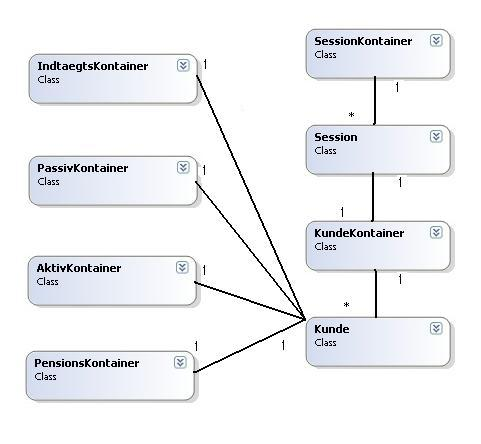
\includegraphics[width=1.0\textwidth]{Billeder/Klassediagram/ClassDiagramHoved.jpg} 
\end{center}
\caption{Klassediagram, Entiteter}
\label{Klassediagramhoved}
\end{figure}

De fire n�ste klassediagrammer viser forholdet mellem en kontainer klasser og den klasse som den er kontainer for. De viser ogs� hvorledes af vi har gjort brug af arv. Diagram \ref{fig:ClassDiagramIndtaegt} kan ses p� side \pageref{fig:ClassDiagramIndtaegt}, \ref{fig:ClassDiagramAktiv} kan ses p� side \pageref{fig:ClassDiagramAktiv}, 
\ref{fig:ClassDiagramPassiv} kan ses p� side \pageref{fig:ClassDiagramPassiv} og \ref{fig:ClassDiagramPension} kan ses p� side \pageref{fig:ClassDiagramPension}.

\begin{figure}
	\centering
		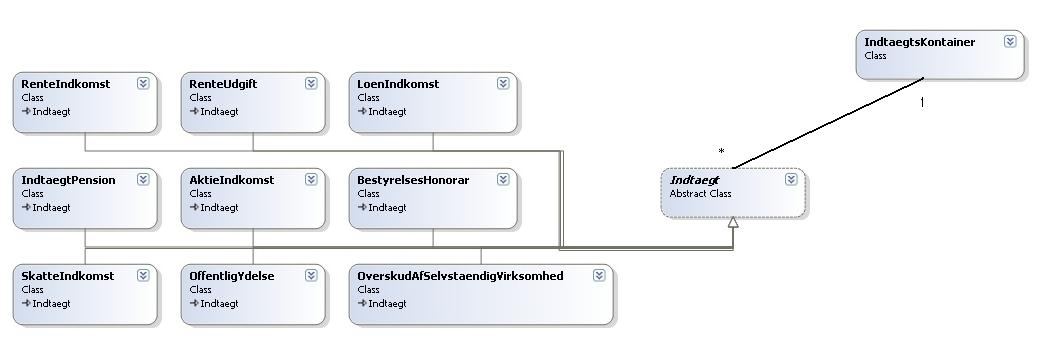
\includegraphics[width=1.00\textwidth]{Billeder/Klassediagram/ClassDiagramIndtaegt.jpg}
	\caption{Klassediagram, Int�gter}
	\label{fig:ClassDiagramIndtaegt}
\end{figure}

\begin{figure}
	\centering
		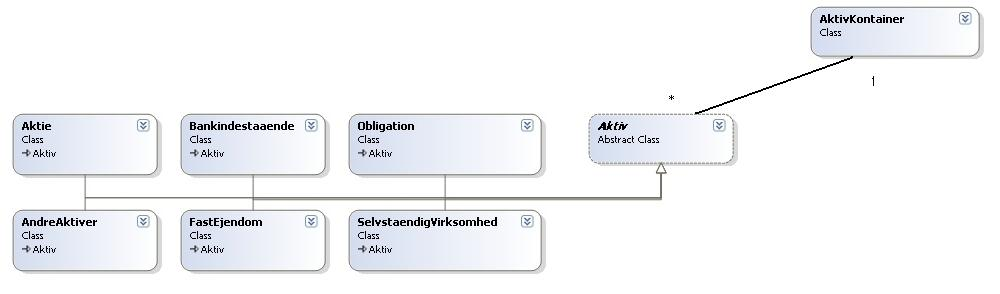
\includegraphics[width=1.00\textwidth]{Billeder/Klassediagram/ClassDiagramAktiv.jpg}
	\caption{Klassediagram, Aktiver}
	\label{fig:ClassDiagramAktiv}
\end{figure}

\begin{figure}
	\centering
		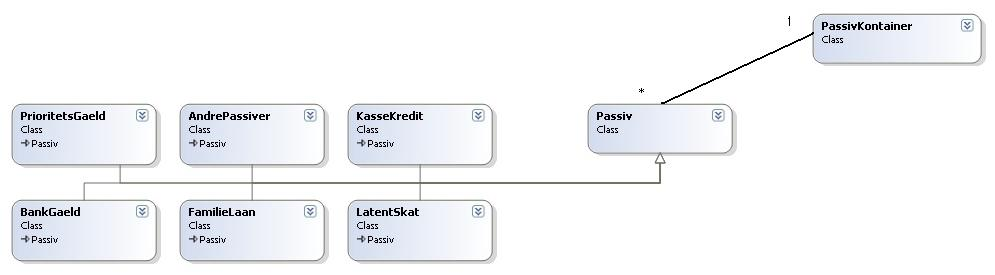
\includegraphics[width=1.00\textwidth]{Billeder/Klassediagram/ClassDiagramPassiv.jpg}
	\caption{Klassediagram, Passiver}
	\label{fig:ClassDiagramPassiv}
\end{figure}

\begin{figure}
	\centering
		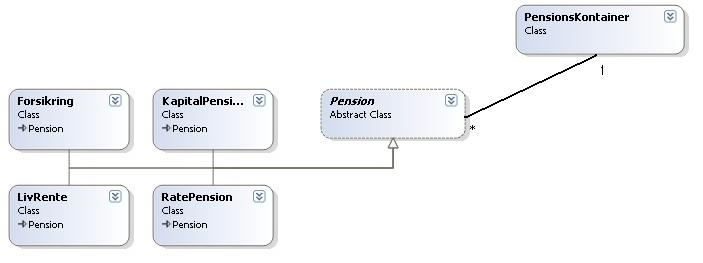
\includegraphics[width=1.00\textwidth]{Billeder/Klassediagram/ClassDiagramPension.jpg}
	\caption{Klassediagram, Pensioner}
	\label{fig:ClassDiagramPension}
\end{figure}

Efterf�lgende var vi et diagram som viser at der en 'kontrol' klasse som hver styer mellem 1 og 3 forme/skr�me. Dette repr�sentere kontrol og view i design patternet MVC, som der kan l�se om i afsnit \ref{MVC} p� side \pageref{MVC}.

\begin{figure}
	\centering
		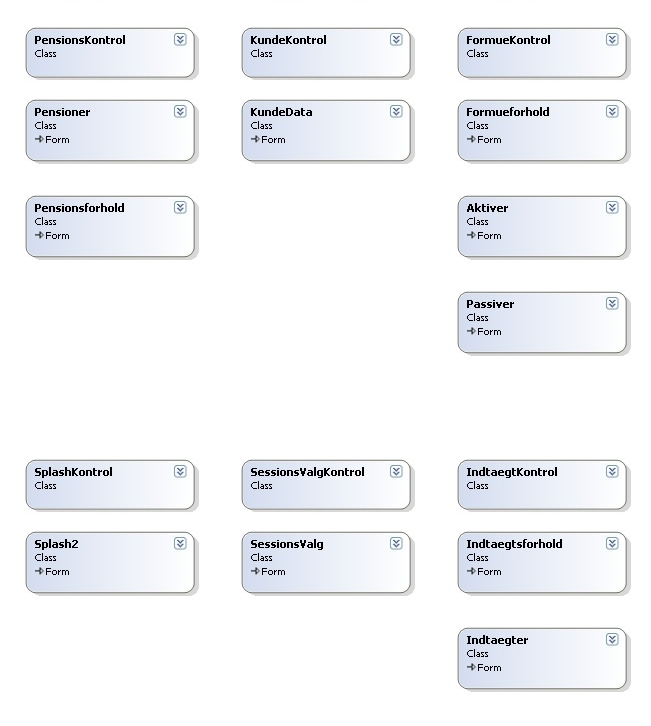
\includegraphics[width=1.00\textwidth]{Billeder/Klassediagram/ClassDiagramGuiKontrol.jpg}
	\caption{Klassediagram, Kontrol, View}
	\label{fig:ClassDiagramGuiKontrol}
\end{figure}

Det sidste klassediagram vi kan byde p� indeholde forskellige klasser. Dette hendler om klassen der tager sig af at kommunikere be databasen, vores post nr. klasse og to klasser som kan bruges til at sortere med. Diagram \ref{fig:ClassDiagramMiscdetaile} kan ses \pageref{fig:ClassDiagramMiscdetaile}.

\begin{figure}
	\centering
		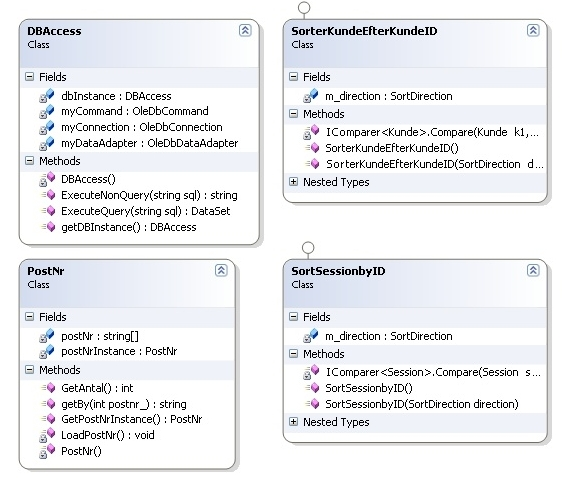
\includegraphics[width=1.00\textwidth]{Billeder/Klassediagram/ClassDiagramMiscdetaile.jpg}
	\caption{Klassediagram, Diverse}
	\label{fig:ClassDiagramMiscdetaile}
\end{figure}

Til sidst vil vi vise de mange af samme diagram, men denne gang med detailer som medlemsvariabler og -metoder.

\begin{figure}
	\centering
		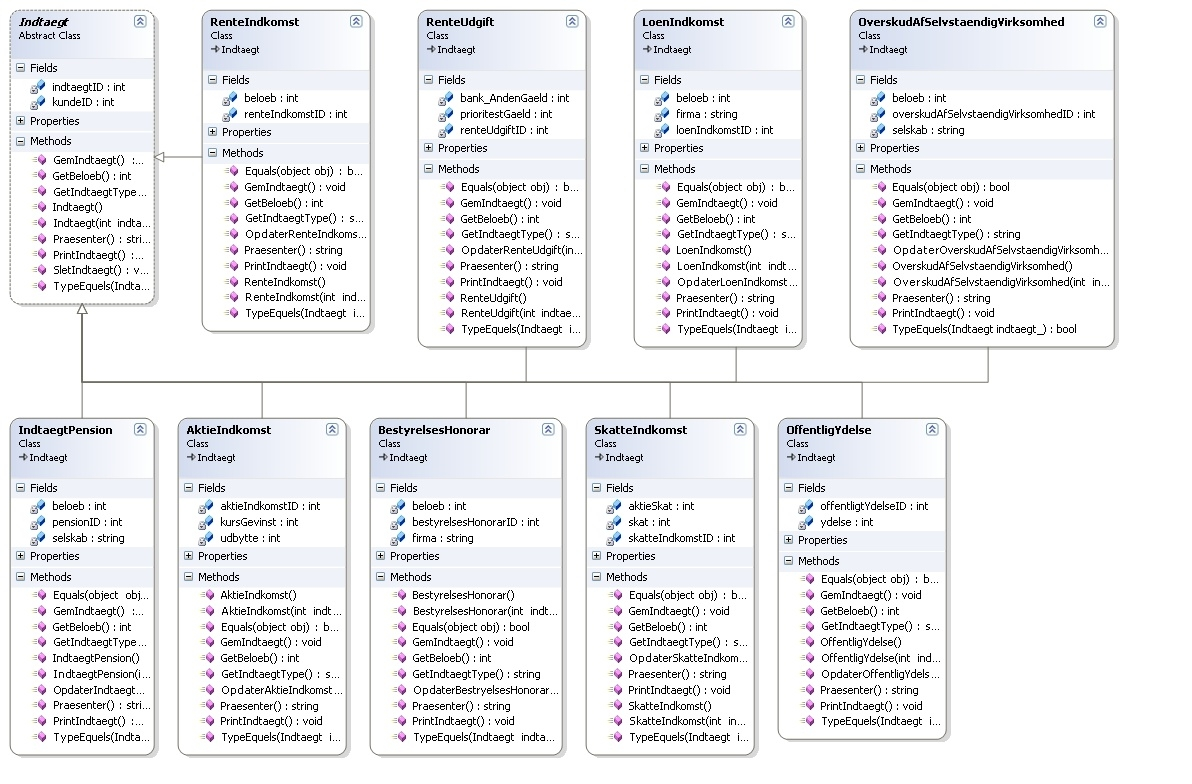
\includegraphics[angle=270, width=1.00\textwidth]{Billeder/Klassediagram/ClassDiagramIndtaegtDetaile.jpg}
	\caption{Klassediagram, Intaegt detailer}
	\label{fig:ClassDiagramIndtaegtDetaile}
\end{figure}

\begin{figure}
	\centering
		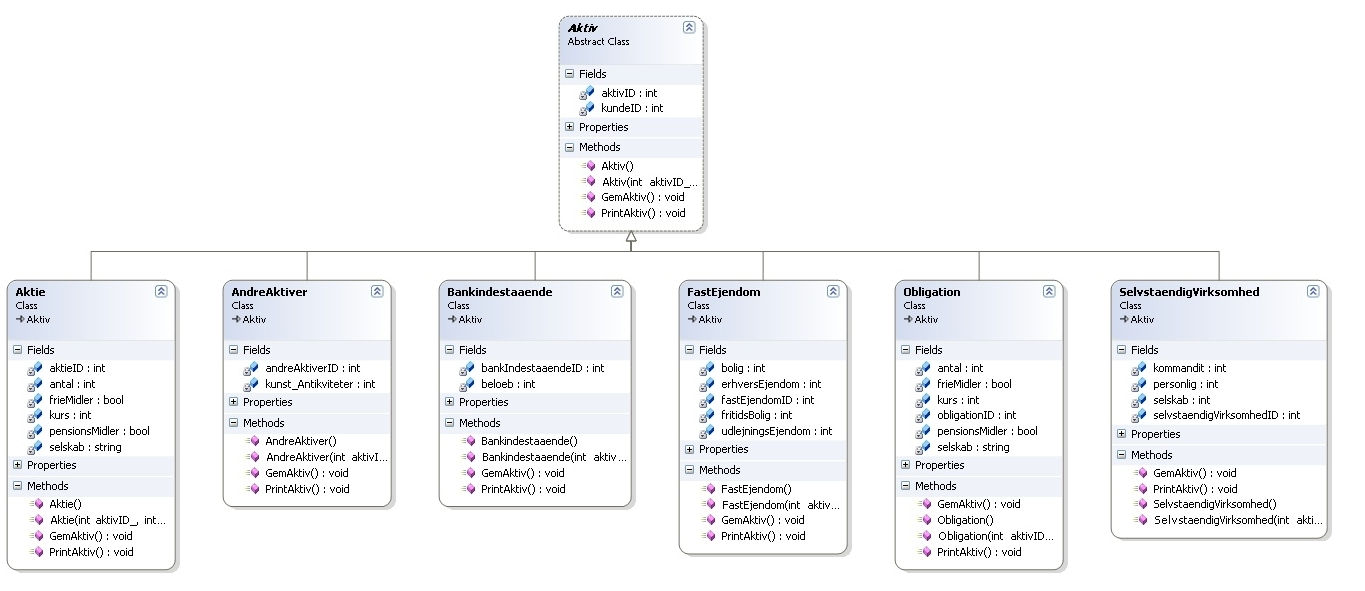
\includegraphics[angle=270, width=0.70\textwidth]{Billeder/Klassediagram/ClassDiagramAktivDetaile.jpg}
	\caption{Klassediagram, Aktiv detailer}
	\label{fig:ClassDiagramAktivDetaile}
\end{figure}

\begin{figure}
	\centering
		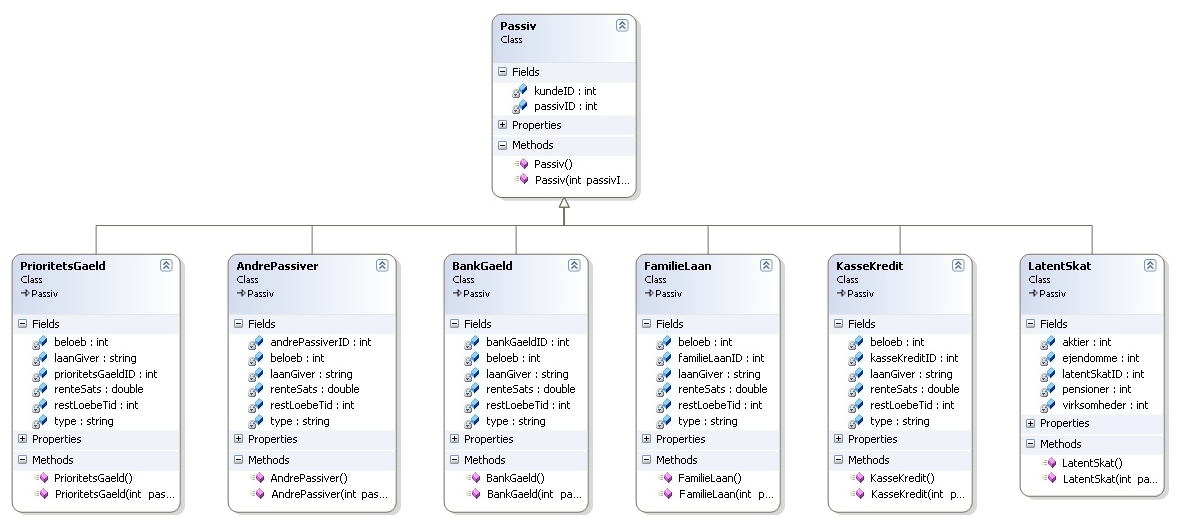
\includegraphics[angle=270, width=0.70\textwidth]{Billeder/Klassediagram/ClassDiagramPassivDetaile.jpg}
	\caption{Klassediagram, Passiv detailer}
	\label{fig:ClassDiagramPassivDetaile}
\end{figure}

\begin{figure}
	\centering
		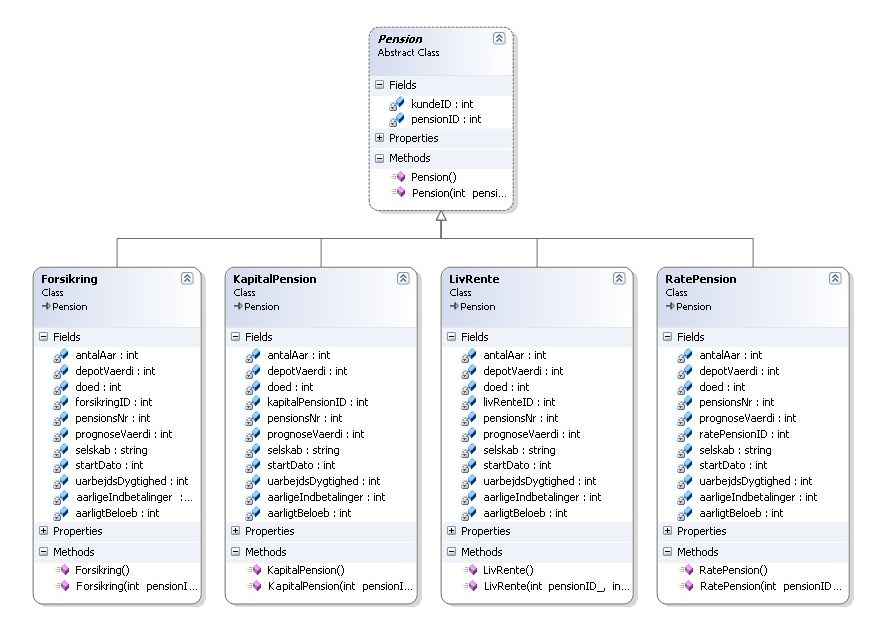
\includegraphics[angle=270, width=0.90\textwidth]{Billeder/Klassediagram/ClassDiagramPensionDetaile.jpg}
	\caption{Klassediagram, Pension detailer}
	\label{fig:ClassDiagramPensionDetaile}
\end{figure}


\newpage
\section{EIK Banks oprindelige opl�g}\label{EIK_Oplaeg}
PRIVATE BANKING V�RKT�J\\

Indledning: Private banking best�r i r�dgivning overfor formuende kunder indenfor investeringspleje, pensions- og skatteforhold, f.eks. i forbindelse med til- og fraflytning udlandet.\\Grundlag: Foruds�tningen for en professionel r�dgivning af kunder indenfor Private Banking er et overblik over kundens - og �gtef�lles indt�gtforhold, formueforhold, arbejdssituation, pensionsopsparing, forsikringsd�kninger samt fremtidige forventninger.\\ Dette overblik skabes i dag via registrering af alle ovenn�vnte oplysninger i Excel, hvorefter overblikket generes. Herefter skal man indtaste fornyede oplysninger for at simulere andre situationer i forbindelse med r�dgivningen af kunden. Dette kan p.t. v�re en besv�rlig proces.\\

Fremtidigt v�rkt�j:
Projektgruppen opgave vil v�re at finde frem til en mere automatiseret l�sning, som kan erstatte det nuv�rende excel ark. \\ Vi kan forestille os f�lgende l�sningsmulighed:\\ En database, hvor kundens oplysningen registreres i forskellige tabeller. \\ En r�kke andre tabeller/databaser med nyttige oplysninger, f.eks. \\

\begin{itemize}
\item offentlige pensioner 
\item test vedr. risikoanalyse vedr. risikoprofil
\item pensions- og d�kningsforhold for de foretrukne samarbejdspartnere/forsikringsselskaber
\item v�rdipapirer over foretrukne portef�ljer, f.eks. Eik Banks modelportef�lje   
\item skatteforhold i foretrukne udlande, f.eks. Frankring, Spanien, England m.fl.
\item g�ngse realkreditl�n, beregningsmotor, oml�gning af l�n
\end{itemize}

Noget af ovenn�vnte kunne t�nkes at v�re links til andre websites.\\

Her ovenp� l�gges et brugerinterface, hvor resultatet af kundens oplysninger vises i pr�sentabel format ( mulighed for udskrift). Det skal endvidere v�re muligt at simulere forskellige muligheder/situationer under m�det med kunden, b�de med hensyn til indt�gtsforhold, pension- og d�kningsforhold, Investeringspleje samt skattem�ssige forhold, dels p� grundlag af kundens egne oplysninger og dels de faste oplysninger, jf. ovenfor. Kunden vil dermed f� et relevant og grundigt overblik/grundlag for at tr�ffe beslutninger.
\newpage
\newpage
\section{Det eksisterende system}\label{Eksisterende}

F�lgende udklip er fra et af de excelark banken bruger og vises her som et eksempel p� det nuv�rende system.\\

\begin{figure}
	\centering
	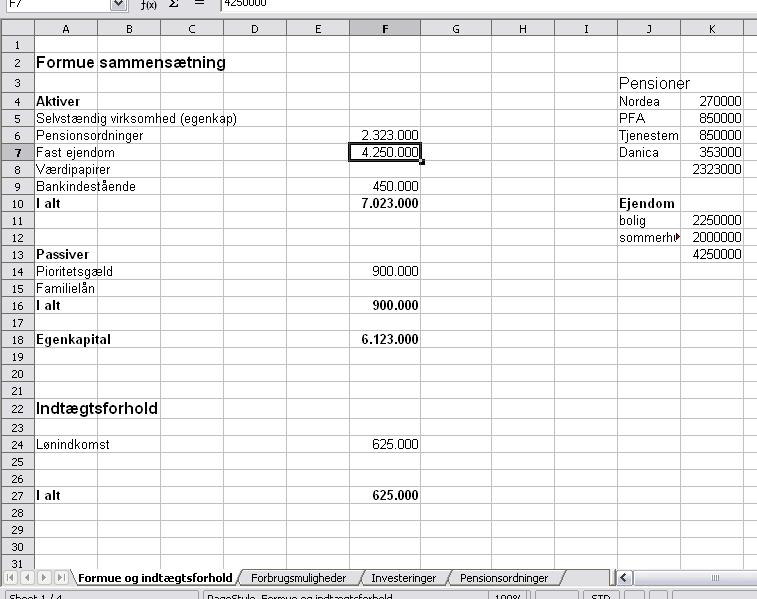
\includegraphics[width=1.00\textwidth]{Billeder/Eksisterende_system/Formue_og_indtaegt.jpg}
	\caption{Formue og indtaegt}
	\label{Formue_og_indtaegt}
\end{figure}
\newpage
\begin{figure}
	\centering		
	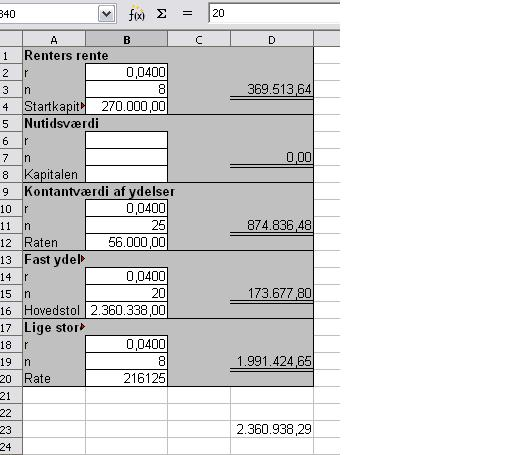
\includegraphics[width=1.00\textwidth]{Billeder/Eksisterende_system/Forbrugsmuligheder1.jpg}
	\caption{Forbrugsmuligheder}
	\label{Forbrugsmuligheder_1}
\end{figure}
\newpage
\begin{figure}
	\centering		
	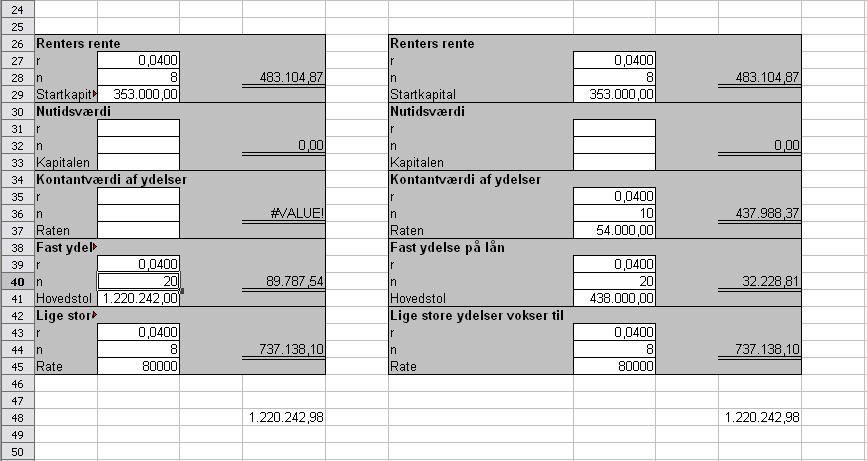
\includegraphics[width=1.00\textwidth]{Billeder/Eksisterende_system/Forbrugsmuligheder2.jpg}
	\caption{Forbrugsmuligheder 2}
	\label{Forbrugsmuligheder_2}
\end{figure}
\newpage
\begin{figure}
	\centering
	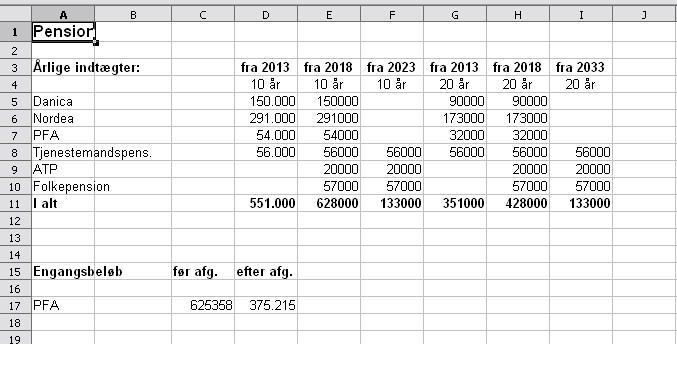
\includegraphics[width=1.00\textwidth]{Billeder/Eksisterende_system/Pension1.jpg}
	\caption{Pension 1}
	\label{Pension_2}
\end{figure}
\newpage
\begin{figure}
	\centering
	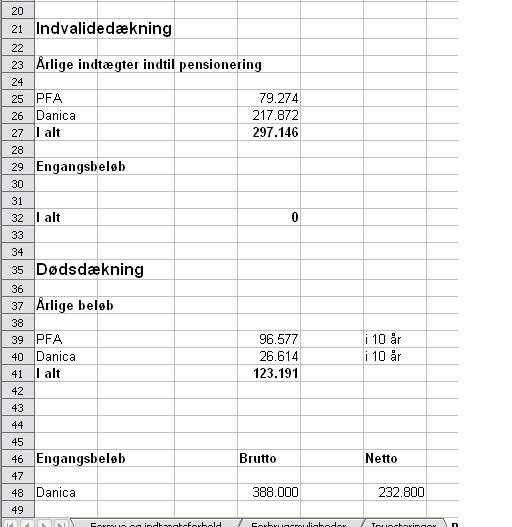
\includegraphics[width=1.00\textwidth]{Billeder/Eksisterende_system/Pension2.jpg}
	\caption{Pension 2}
	\label{Pension_2}
\end{figure}
\newpage









\newpage
\section{Morgenm�der}\label{Morgenmoeder}
\paragraph{Morgenm�de 24-01-06}

\begin{itemize}
\item Karakteristik af EIK: Ikke EDB-kyndige medarbejdere, brugere p� normalt nivau.

\item Valg af database?
Access indtil videre. Da der ikke bliver meget pres p� med 4 medarbejdere. Det ligger ogs� i kortetene at vi b�r g� efter en kostfri l�sning. Afpr�v en simpel database p� EIK filserveren.

\item Webservice?
Kan filserveren bruges til webservices

\item Rapportstruktur:
Kig gamle rapporter igennem.

\item Latex rapport header:
Lav en header til texfilerne til rapporten.

\item Videoproto af private banking session:
F� Dion til at vise hvordan et realistisk kunderforl�b ser ud. Se nuv�rende arbejdsgange og f� ham til at s�tte ord p� de nuv�rende problemer.

\item Lave en tidsoversigt:
Lave en tom 'skal' over tidsforl�bet.

\item Login delen:
P�begyndelse af logindelen er en mulighed allerede nu.

\item Kigge p� mulige faldgrupper i forl�bet som det ser ud nu (mild risikoanalyse).

\item Fastl�gge filosofierne:
\begin{itemize}
\item Crack the hardest nut first.
\item 'Stille dumme sp�rgsm�l filosofien' Ingen sp�rgsm�l er for dumme. Modvirker kommunikationsvanskeligheder.
\item KISS-Keep It Simple Stupid / KISBI: Keep It Simple But Intelligent
\end{itemize}

\item Fastl�gge arbejdsformerne:
Spiralmodellen.
Daglige m�der efter Scrum-forbillede.
Der er 7 iterationer. 1 uge er planl�gning og installation. Sidste 2 uger er til rapportskrivning.
K�re efter fastlagte ugentlige m�l. Det kan v�re et delsystem eller en papirmodel. el. M�let skal v�re f�rdigt n�r vi g�r hjem torsdag.
Afholde et ugentligt informationsm�de med EIK kontakterne. Prim�rt for at vise fremskridtet, engagement og for at hindre at vi kommer for langt ud p� et sidespor. Dette ugentlige m�de afholdes fredag formiddag (11-11.30 tiden).
NOTE: Vi skal informere EIK medarbejdere p� forh�nd om hvor meget tid vi regner med at der g�r ved samtaler og andre sessioner.
\end{itemize}


\paragraph{Morgenm�de 26-01-06}

Deltagere: Klaus, Jes og Christian

\begin{itemize}
\item Ting der skal ske i dag 26-04-06
\begin{itemize}
\item 1.Afklaret om hvorvidt vi kan g�re bruge en database server.
\item 1.Vi skal have Johann til at tjekke med SDC hvilke ting vi kan f� lov til p� deres file-server, og hvilket OS den k�re.
\item 2.Hvis der er Win2003Server om vi s� kan bruge IIS (som enten er instelleret eller som vi m� installerer) (dette skal unders�ges).
\item 3.Der er m�de mellem EIK og SDC p� mandag.
\item 4.Hvis ikke vi kan bruge en database server, s� bruger vi bruge en access database p� et delt netv�rks-drev.
\item 2.Afklaret om hvorvidt vi kan lave en web-server p� deres file-server. Ene og alene for at give os selv s� mange udviklings muligheder som muligheder.
\item 3.Noterne fra m�det i g�r med Dion (video session) skal skreves sammen, for at fjerne dublikater.
\item 4.Kort snakke om det m�de med Dion for at sikre at vi har samme opfattelse.
\item 5.Lave en skabelon/disposition til fredags m�det med EIK.
\end{itemize}

\item Ting som tidligst skal laves fra om fradagen d. 27-01-06
P� baggrund af video-session, Detaljeinformationsbehov (liste fra Dion 24-01-06) og regneark kan vi udf�rdige prototyper.
\end{itemize}
\paragraph{Morgenm�de 27-01-06}

Deltager Klaus, Jes og Christian.

Dagsorden.

\begin{itemize}
\item Der skal bestilles papir artiker.
\item Vi skal have planlagt n�ste uge.
\item Vi skal have Kim til at prioritere deres krav til systemet, samt at klarl�gge vigtigheden af pensionsdelen.
\item Opsummering af fredagsbriefing med EIK.

\item Forberedelse til LoFi Prototyping session:
\begin{itemize}
\item 830-930	Gennemg� materiale (Excel ark, printede regneark)
\item 930-1300	Kreativt stadie.  Form�l: En masse kreative tanke. OVERORDNET!
\item 930-1030	Individuelt udarbejde en l�sning i LoFi.  
\item 1030-1145	Vurdering i plenum. Diskuter for og imod.
\item 1145-1230	Frokost
\item 1230-1300	Beslut p� baggrund af diskussionen hvad der er den bedste l�sning.
\item 1300-1430	Konstruer prototypen.
\item 1430-1600	Uddeleger roller, og planl�g sessionen (foretages tirsdag kl 9.30)
\item 1600-	Afslut dagen. Opsumer i dagbogen.
\end{itemize}
\end{itemize}
\paragraph{Morgenm�de 01-02-2006} 

\begin{itemize}
\item Der skal sammenlignes indtryk og noter fra de 2 LOFI prototype-sessioner vi har afholdt og de indsamlede data skal analyseres og sammenfattes.
\item Problemformuleringen er oprettet som dokument under 'Rapport' og skal skrives f�rdig.
\item M�de med Dion er booket til i morgen torsdag (02-02-06) hvor vi skal have et crash-kursus i pensionsteori kl 14.
\item Planl�gningen af fredags-briefing p�begyndes.
\item Vi skal kigge n�rmere p� at specificere krav og afgr�nsninger til og af systemet. Det samme g�r sig g�ldende med at 'kn�kke den h�rdeste n�d f�rst'. Dette skal vi komme n�rmere ind p�, vi skal identificere den h�reste n�d.
\item Det er ved at v�re p� tide at vi kommer i gang med rapportskrivning. Her t�nkes specielt p� virkomshedsprofil, indledning og problemformulering.
\item P� fredag skal n�ste uge planl�gges.
\item N�r fredags-briefing er overst�et skal vi have en snak med Pia om projektet, produktet og systemudviklingen.
\item Vi skal huske at drikke nogle bajere efter arbejdstid p� fredag, vigtigt at f� tankerne lidt v�k.

\item Tilf�jelse:
Ide: For at indsamle krav til pr�sentationsdelen af applikationen kunne der afholdes en brainstorming session/m�de med Dion og Kim. Vi skal sk�re ind til benet og f� de vigtige ting p� banen. Hvad skal en pr�sentation for kunden indeholde. Hvilke grafer og p� hvilke tal skal graferne laves. Vi skal arbejde os hen imod at f� specificeret de enkelte indtastningsfelter i applikationen. 
\end{itemize}
\paragraph{Morgenm�de 03-02-06}

Deltagere Klaus, Jes og Christian\\

Planl�ge n�ste ugens forl�b.
Opsamling p� samtalen med Pia.
Opsamling p� fredags brifing
\paragraph{Morgenm�de 06-02-06}

Plan for i dag\\

Vi skal unders�ge om det er planen at der bliver rene indtastnings opgaver for sekret�rerne.
Der skal laves nye og p�ne items til den n�ste prototype. Dette g�r Jes og Christian i gang med.
Vi skal have diskuteret vore mappe struktur og placeringen af vores filer. Der er en reel risiko for at miste overbliket over alle vores noter.
Vi skal kigge n�rmere p� at identificere den h�rdeste n�d - dette skal vi komme n�rmere ind p�.



\paragraph{Morgenm�de 07-02-06}

Plan for i dag\\

Vi skal have diskuteret vore mappe struktur og placeringen af vores filer. Der er en reel risiko for at miste overblikket over alle vores noter.
Den nye prototype skal laves f�rdig, s� den er klar til brug ved session.
Principper og problemformulering skal behandles.
Vi skal have booket prototype-m�de, vi afs�tter en time til sessionen.
Alt efter hvor meget tid vi har til overs kan vi kigge n�rmere p� et studieomr�de og endvidere f� skrevet noget ned om prototyping.
\paragraph{Morgenm�de 08-02-06}

Plan for i dag\\

Kigge n�rmere p� et studieomr�de.
Endvidere f� skrevet noget ned om prototyping.
Problemformuleringen skal vi ordentlig i gang med.
Kigge p� Latex. Ang skrive afsnit sammen (Bibtex).
Misc.
\paragraph{Morgenm�de 08-02-06}

Deltagere: Klaus, Jes og Christian\\

Alle noter skal skrives ind.
Vi skal have skrevt vores tanke ind i prototyping dokumenter, omkring det netop afholde session.
Vi skal have lagt lyd og billed fra session skal l�gges op til deling.
Vi skal have indkaldt til fredagsbrefing.
\paragraph{Morgenm�de 10-02-06}

Dagsorden\\

Planl�gge og afholde fredagsbriefing.
Sammenskrivning af noter fra session 3.
Rapport-skrivning: Problemformulering,
Oprydning i mappe-strukturen.
Snakke om MVC og arkitektur.
Planl�gge uge 7.
Unders�ge muligheder for litteratur til studieomr�det.
Indledende tanker omkring n�ste uges design-fase.



\paragraph{Morgenm�de 13-02-06}

Dagsorden\\

Tage hul p� design.
Identificering af klasser
Strukturdokument (navnekonventioner)
Snakke om MVC og arkitektur.
Unders�ge muligheder for litteratur til studieomr�det.
Database tilgang unders�ges.
Test MVC-templaten af.
Skrive om MVC.



\paragraph{Morgenm�de 14-02-06}

Dagsorden\\

Database tilgang unders�ges: Kompilere dbTest og smide det p� EIKserveren for at teste det.
Tage hul p� design.
Identificering af klasser
Strukturdokument (navnekonventioner)
Snakke om MVC og arkitektur.
Unders�ge muligheder for litteratur til studieomr�det.
Skrive om MVC.




\paragraph{Morgenm�de 15-02-06}

Dagsorden\\

S�fremt at Johann er rask og p� arbejde, skal vi teste db tilgang mellem hans maskine og filserveren.
Design: Objekt-identifikation $\rightarrow$ pre-state klassediagram.
 
Navne-konventionering.
		
\paragraph{Morgenm�de 16-02-06}

Dagsorden\\

S�fremt at Johann er rask og p� arbejde, skal vi teste db tilgang mellem hans maskine og filserveren.
Mapping til DB -> DB-diagram.
Arv i forbindelse med C\# og DB.
Navnekonventionering.
Oprette et C\# projekt i Visual og samle de forberedte entitetsklasser.
Vi skal have fat i Kim ang�ende sp�rgsm�l i forbindelse med Pensionsforhold (popup), samt Obligationer.
Forberede fredags-briefing.


\paragraph{Morgenm�de 17-02-06}
 
Dagsorden\\

Forberede og afholde fredagsbriefing.
Hvis Johann er blevet rask $\rightarrow$ test DB.
Fredag er prim�rt en skrive-dag, hvilket betyder at vi skal arbejde med rapporten.
Problemstillingen/er, en mere specifik beskrivelse af dette omr�de.
Design patterns, observer m�nstret og vores form�l med at bruge design patterns.
Uddybning af de resterende omr�der.
Principperne for mapping af DB og vores valg af princip.
Planl�gning af n�ste uge (uge 8).
\paragraph{Morgenm�de 20-02-06}

Dagsorden\\

Der skal kigges p�/kodes kontainer-klasser til entitetsklasserne, og kunde \& session skal kodes.
Databaseproblematik; performance (hvorn�r/hvor ofte skal der l�ses fra db'en, hvor skal denne tilgang ligge?)
\paragraph{Morgenm�de 21-02-06}

Dagsorden\\

Navnekonvention: Alle reserverede SQL ord i query's skrives med stort.
Kode
GUI: dynamisk indhold p� Aktiver, Passiver, Indt�gter og Pensioner.
Generel kodning af systemetet
Hvordan f�r h�ndterer vi lister (dataudtr�k, s�gning og sortering)
Session \& kunde


\paragraph{Morgenm�de 22-02-06}

Dagsorden\\

Jes skal opdateres.
De resterende kontrol-klasser skal laves.
De resterende entitets-klasser skal kobles sammen med Kunde.
Database-klassen skal laves som en singleton. Hertil skal der skrives i rapporten, samt klarg�res et eksempel.
Hver kunde skal kunne loade sine Indtaegter, Aktiver, Passiver og Pensioner.
\paragraph{Morgenm�de 23-02-06}

Dagsorden\\

Kode
Lav 'gem-i-database' strukturen.
Videre kodning af 'hent-fra-database' strukturen, som blev lavet i g�r.
Bestemme hvordan programmet skal starte, hvad skal der ske n�r programmet starter, 'velkomstsk�rm' $\rightarrow$ lave en opstartsform.

Lavet og udsendt menu til fredagsbriefing.
\paragraph{Morgenm�de 24-02-06}

Dagsorden\\

Afholde fredags-briefing.
Opdatering af klassediagram i forhold til kode og opdatering af kode (navngivning).
Oprydning i dokumenter/filer.
Skrive-dag:
Database (normalisering, hvordan der skal gemmes etc.)
Indledende til projektet (problemstilling etc.)
Bedre/mere specifik beskrivelse af krav.
Bedre/mere specifik beskrivelse af afgr�nsninger.

Tale mere om afgr�sning af projektet.
\paragraph{Morgenm�de 27-02-06}

Dagsorden\\

Notesystemet: Afgr�nsning / en mulighed for at 'shine' systemet lidt op.
Hvordan ser startsiden til systemet ud? Man skal v�lge en tidl session eller starte en ny.
Kodning:
Load/save funktionerne skal f�rdigg�res. Skal denne funktion optimeres?
F�rdigg�relse af et sk�rmbillede og bruge det som skabelon til resten af systemet. Ogs� med henblik p� fremvisning af system p� fredagens briefing.
GUI. Begynde med velkomstsk�rmen. K�de teorien sammen med systemet.
Forberede noget til Pias bes�g.

\paragraph{Morgenm�de 28-02-06}

Dagsorden\\

Kodning
Opstarts screen skal forbedres. Navigeringen skal f�rdigg�res.
Overordnet design
Skal der sendes hele 'sessions' objekter mellem alle klasserne?
Pia kommer idag. 
Vi skal snakke om hvad der specifikt skal st� i rapporten. Opbygningen / struktur af rapporten, hvor meget skal det ene og det andet emne fylde (f.eks Fokusomr�det GUI og til dels Design Patterns).
Vi skal snakke afgr�nsning af systemet og dets funktionalitet.
\paragraph{Morgenm�de 28-02-06}

Dagsorden\\

Arbejde videre med fremsending af Sessionsobjekt.
Note skal l�ses ind i kundedata-formen.
Kod videre.
\paragraph{Morgenm�de 02-03-06}

Dagsorden\\

Indbydelse til fredags-briefing skal laves og fremsendes.
SaveKunde funktionen skal tjekkes igennem, da der er mistanke om fejl i denne funktion, der skal formentlig sendes et sessionsid med over.
Der skal arbejdes med 'Indtaegtforhold' og dens popup 'Indtaegter'. Vi tager udgangspunkt i �n af indtaegtforholdende og koder den igennem.



\paragraph{Morgenm�de 03-03-06}

Dagsorden\\

Afholde fredagsbriefing: demo af applikationen.
Skrive-dag:
Klaus har noget til DB
Polymorfi
Pias noter/forslag/input/meninger/id�er/


Pr�ve at booke et m�de med Kim og Dion for at f� kvantificeret krav.

Kode
Der skal arbejdes med gem-algoritmen



\paragraph{Morgenm�de 06-03-06}

Dagsorden\\

Kvantificering af krav med Kim og Dion. Forberede m�de. Book et m�de til tirsdag eftermiddag. CRUD (create/read/update/delete) funktionalitet. 
Research GUI / print.
Kode
Print funktionalitet.
GUI funktionalitet. 
De 10 gode r�d. 
Treeview. inkl. fejlcheck. Lav en algoritme.

Kommende dage:
Skrive noget om polymorfi.
\paragraph{Morgenm�de 07-03-06}

Dagsorden\\

Kvantificering af krav med Kim og Dion kl 14. Forberede m�de. Bruge kravslisten. Smid CRUD p�.
Research GUI / print.
Kode
Kigge p� Factory Design Patterns. 
Print funktionalitet.
Lave en eksperten. 
GUI funktionalitet. 
De 10 gode r�d. 
Treeview. inkl. fejlcheck. Lav en algoritme.

Evt / Kommende dage:
Skrive noget om polymorfi.
\paragraph{Morgenm�de 08-03-06}

Dagsorden\\

Noter til m�de med Kim, Claus og Dion.
Research GUI  - finde Bogen / print.
Kigge p� Factory Design Patterns. 
Print funktionalitet.
Check op p� Eksperten sp�rgsm�l, hvordan portes objekt med serialisation til XML og tilbage igen.
GUI funktionalitet. 
De 10 gode r�d. 
Treeview. Update mangler. Hvordan for vi sat bel�b p� p� oversigt under Indt�gtsforhold.
Vi skal have lavet en kravliste. Skal have d�kket alle funktioner i programmet ind med krav.
Have lavet et udkast hvordan rapporten fra udprintdelen af systemet kunne se ud.

Evt / Kommende dage:
Skrive noget om polymorfi.
\paragraph{Morgenm�de 09-03-06}

Dagsorden\\

Videre med Crystal Reports og XML serialization.
Knap til at tilf�je en post p� 'Indtaegter' der ikke lukker vinduet.
Treeview problemet skal l�ses.
Implementation af reglerne for hvorn�r elementer p� brugergr�nsefladen skal v�re synlige/brugbare (impl. de 10 regler i vores GUI).
GUI litteratur.
Kigge p� 'abstract factory' design patterns.
Forberede og udsende invitation til fredagsbriefing.
\paragraph{Morgenm�de 10-03-06}

Dagsorden\\

Fredagsbriefing.
Skrivedag.
Skrive om GUI / HCI.
Polymorfi / arv.
Opdatere design Patterns generelt, se vores gamle Design Patterns aflevering
Checke op p� dokumentet fra Pia m�det.
Rydde op i vores dokumentstruktur.
Arbejde videre med Crystal Reports.



\paragraph{Morgenm�de 14-03-06}

Dagsorden\\

Videre med Crystal Reports og dertilh�rende dataset.
Vi skal have lagt rediger og slet p� Indt�gtsformen.
GUI regler skal implementeres.
GUI design.
�ndre fra r�dgiver til kundenavn p� 'tidl session'.



\paragraph{Morgenm�de 14-03-06}

Dagsorden\\

Videre med Crystal Reports og dertilh�rende dataset.
Rediger-funktionalitet p� Indt�gtsforhold.
GUI regler skal implementeres.
GUI design.
Kommentering af koden.



\paragraph{Morgenm�de 15-03-06}

Dagsorden\\

Videre med Crystal Reports. Hvis ikke at vi kan f� det til at virke som vi har foresl�et at det skal virke, dvs. med flere koloner, s� kunne vi lave �n rapport pr kunde. 
//Vi kan/skal unders�ge hvordan man s�tterdynamiske felter p� rapporten.
Vi er blevet enige om at vi laver en rapport pr kunde.
GUI regler skal implementeres. Vi mangler indt�gter, login og sessionv�lger.
GUI design. Vi skal finde ikoner til vores knapper. Og vi skal efterleve gestalt lovene.
Kommentering af koden. Der mangler kommentarer til indtaegt og til en af dens subklasser.
Vi har haft en diskution om hvorvidt alt kodning skal lukkes p� fredag d. 17-03-06 eller om GUI design skal v�re �ben for forandringer i forbindelse med at vi bliver klogere p� det omr�de. Klaus mener at alt kode skal v�re lukket og at vi i rapport m� skrive hvad vi kunne have gjort bedre med henhold til GUI. Jes og Christian vil gerne holde GUI �ben s� �ndringerne kan blive lavet sidel�benede med at vi bliver klogere. Vi diskuterer dette igen efter frokost.



\paragraph{Morgenm�de 16-03-06}

Dagsorden\\

Crystal Reports:
Vi er blevet enige om at vi laver en rapport pr kunde.
Prim�rt m�l: Vi skal have noget simpelt data ud - vi forventer at ende med en skrabet version af rapporten.
Vi skal have h�rt vejleder Pia om hvordan man b�r forholde sig til et krav fra en virksomhed, som ikke kan l�ses/ikke kan l�ses fuldst�ndigt. Hvordan b�r man forholde sig i forhold til skolen (NB) og i forhold til virksomheden (EIK).
GUI regler skal implementeres. Vi mangler sessionv�lger. (slet og rediger i Indt�gtsforhold bliver ved med at v�re synlige, selv n�r der ingen indt�gt er).
GUI design. Vi skal efterleve gestalt lovene. (beskrive disse gestalt love). Skal implementeres ogs�.
Kommentering af koden. Der er skrevet kommentarer til det meste kode, de skal dog generelt g�s igennem og rettes til hvor n�dvendigt. Der mangler bla parameterlister og beskrivelser af disse, samt beskrivelser af hvad non-void funktionerne returnerer.
Vi skal indkalde til Fredags Briefing.
Her skal der tages stilling til om vi vil holde flere fredagsbriefings. Dette skal kommunikeres ud til EIK p� fredagsbriefingen.
Forslag: At udlevere hvad vi har skrevet af rapport indtil videre og lade dem l�se det igennem. Vi kunne evt. afholde m�de mandag hvor vi kunne tage imod evt. kritik.
Vi b�r nok ogs� afholde en lille session hvor tester programmet af med de kommende brugere. Vi b�r m�le fremgangen i forhold til tidl. arbejdsgange, og lade dem teste programmet lidt af.
\paragraph{Morgenm�de 17-03-06}

Dagsorden\\

Crystal Reports:
Formatering af rapporten. Venstrestilles.
Fredags Briefing skal afholdes.
Skrive noget om prototyping. 
Rydde op i mappestrukturen. Opstarte med at skrive i Latex. Se hvor mange sider vi har allerede?
GUI regler. TABs. (slet og rediger i Indt�gtsforhold bliver ved med at v�re synlige, selv n�r der ingen indt�gt er).
GUI Design gestalt lovene.
Kommentering skal der arbejdes lidt mere p�. Skal nok g�es lidt igennem. Mangler m�ske parametre nogen steder. (lav prioritet, evt f�rst efter forl�bet her er afsluttet).


ANG: Fredags Briefing.
Her skal der tages stilling til om vi vil holde flere fredags briefings. Dette skal kommunikeres ud til EIK p� Fredags Briefingen.
Forslag: At udlevere hvad vi har skrevet af rapport i den sidste del af ugen og lade dem l�se det igennem. Vi kunne evt. afholde m�de mandag hvor vi kunne tage imod evt. kritik.
Vi b�r nok ogs� afholde en lille session hvor tester programmet af med de kommende brugere. Vi b�r m�le fremgangen i forhold til tidl. arbejdsgange, og lade dem teste programmet lidt af.
\paragraph{Morgenm�de 20-03-06}

Dagsorden

Det sidste afsnit i prototyping skal gennemg�s. Dermed b�r Prototyping v�re t�t p� at v�re f�rdigt.
Samle op p� 1. h�nds noter og vores dokumenter generelt.
Finde ud af hvad vi skal bruge som r�d tr�d (gennemgangs-eksempel)
Virksomhedsprofil, indledning, problemstilling- og formulering.
Principper: Hvordan er det s� g�et med at bruge disse principper?
Studieomr�de dokumentet.
Database dokumentet.
Test: hvad skal bruges som testmateriale: Databasetilgang, gem-algoritmen.


Fra i dag, det vil sige nu, skriver vi direkte i latex-dokumenterne.
\paragraph{Morgenm�de 21-03-06}

Dagsorden\\

Finde ud af hvad vi skal bruge som r�d tr�d (gennemgangs-eksempel).
Arrangeret test af applikationen med brugere.
Studieomr�de dokumentet. (GUI \& Design patterns).
Principper: Hvordan er det s� g�et med at bruge vores principper?
Generel genneml�sning af rapporten, og rette fejl i den.
Test: hvad skal bruges som testmateriale: Databasetilgang, gem-algoritmen.


\paragraph{Morgenm�de 22-03-06}

Dagsorden\\

Der skal laves et gennemgangseksempel (r�d tr�d).
Test-sessionen skal forberedes.
Generel rapport-skrivning til de forskellige afsnit.
Evaluering af vores brug af de principper vi har defineret.
Studieomr�der.
Systemudviklingsmetode.
Test, her kan vi beskrive hvad vi har gjort indtil videre.

De sidste rettelser fra i g�r skal tilf�jes.
\paragraph{Morgenm�de 23-03-06}

Dagsorden\\

Test-sessionen skal forberedes.
Problemformuleringen skal der styr p�.
Konklusion opstartes, og rettes hen i retning af problemformuleringen.
Crystal reports / udprintsfunktionalitet skal der skrives om.
Design af Brugergr�nseflade. Hvor skal vi hen med dette punkt?
Generel rapport-skrivning til de forskellige afsnit.
\paragraph{Morgenm�de 24-03-06}

Dagsorden\\

Test-sessionen skal forberedes.
Test sessionen med deltager Kim skal afholdes.
Vi skal have sendt rapporten ud til Pia og EIK medarbejderne Johann, Dion, Kim.  
Hvor ligger vores hovedproblemer:
Hovedstudieomr�det GUI, vi skal have skrevet en sm�re til det emne. 
Vi skal have skrevet et dokument omkring udprintfunktionaliteten.
Det volder ogs� en del problemer at beskrive vores process, alts� hvilke valg vi traf p� hvilket tidspunkt, og hvorfor vi traf dette valg.
\paragraph{Morgenm�de 27-03-06}

Dagsorden\\

Feedback p� rapporten (rapporten har v�ret smidt ud til Johann og Kim og Pia).
Skrive.
Beskrive vores metode ud fra undervisningsbogen. Alts� bruge skabelonen fra SiP undervisningen til at beskrive vores metode. Bygge det op p� denne m�de: Beskrive hvordan den teoretisk er bygget op og derefter fort�lle hvordan og hvorn�r den er blevet brugt.
Vi skal have skrevet et dokument omkring udprintfunktionaliteten.
Vores process, alts� hvilke valg vi traf p� hvilket tidspunkt, og hvorfor vi traf dette valg.
\paragraph{Morgenm�de 28-03-06}

Dagsorden\\

Feedback p� rapporten (rapporten har v�ret smidt ud til Johann og Kim og Pia). Vi mangler Kim, Pia og lidt Johann.
Skrive.
Vi skal have skrevet et dokument omkring udprintfunktionaliteten.
Nogle af dokumenterne har for lange afsnit. De skal laves l�sevenlige ved at s�tte afsnit ind.
Afrundinger p� de 'f�rdige' dokumenter.
Prototyping. Manglende afsluttende evaluering.
Testsessionen skal afsluttes.
Rydde op i kravslisten.
Mantra: Vores process, alts� hvilke valg vi traf p� hvilket tidspunkt, og hvorfor vi traf dette valg.

\section{Dagb�ger}\label{Dagboeger}
\paragraph{I dag d. 23-01-06}

\begin{itemize}
\item Skal have overblik over rapporten. Hvordan er vores forestilling om den overordnede struktur. Der skal v�re fyld til 100 sider (puha :). Vi skal i gang med at skrive p� rapporten med det samme og skal absolut ikke vente til sidst med at g� i gang.
\item Vi har snakket om at vi skal kunne tage udgangspunkt i de forskellige omr�der n�r vi diskuterer, eller rettere fors�ge at adskille de forskellige omr�der: analyse, design, implementering. Fordelen er f.eks at vi ikke begr�nser vores kreative tankegang af sn�vre kodetankegange i en analyse situation hvor kreative muligheder skal udforskes. Alts� skal vi fors�ge at v�re mere bevidste p� hvilken situation vi befinder os i og tage den rette kasket p�. Alts� ikke noget med at tage analysekasket OG implementeringskasket p�. OFTE FORUDS�TTER DE FORSKELLIGE SITUATIONER HINANDEN OG B�R DERFOR UDF�RES I GENSIDIGT SAMSPIL ;)
\item Vi opfatter hver is�r de svar vi f�r forskelligt, hvilket kan ses som et resultat af d�rlig m�de-teknik og/eller som et resultat af et kommunikationsvanskeligheder (i gruppen og mellem EIK og os).
\item Vores m�de i dag var alt for uprofessionelt, vi skal foreberede os bedre (roller, ikke snakke i munden p� hinanden, have sp�rgsm�l klar f�r m�det, f�lles agenda). 

\item Vi har allerede nu en klar forestilling om at vi skal have en database ind over vores l�sning. Efter at have taget en lille samtale om fordele og ulemper med database eller ej.
\item EIK har en filserver, som databasen kan k�re p�. Dette skal testes.
\item Vi har ogs� l�st snakket om hvilke SU-metoder der skal indover udviklingsforl�bet. Der er stemning for eksperimentel prototyping og brug af UML.
\end{itemize}

\paragraph{I dag d. 24-01-06}

\begin{itemize}
\item Applikationsorienteret:\\
Vi er blevet usikre p� om en databaseret l�sning overhovedet kan lade sig g�re, da den p�g�ldende filserver findes ude p� SDC.

\item Vi har lavet en plan for ugen.
\item Aftalt m�de med Dion: Gennemgang af nuv�rende forl�b med video for at fastholde.
\item Der er blevet udarbejdet en tidslinie vi kan kigge p� og overskue hvor langt vi er n�et i forl�bet.
\item Der er blevet lavet en header i Latex til rapporten.
\item Der er blevet udarbejdet en udviklingsmodel for projektforl�bet.
\item PopstGreSQL Test database installeret p� vores PIII serveren i vores lokale.
\end{itemize}

\paragraph{I dag d. 25-01-06}

\begin{itemize}
\item Vi har installeret postgresql p� klaus's maskine og p� serveren. Vi kan komme i kontakt med klaus's postgres, men ikke den p� serveren.

\item Vi mangler CD'en til windows 2003 server, som skal bruges til at installere IIS p� serven. Denne CD skulle v�re klar til i morgen. S� kan vi teste om vi kan bruge web-services.

\item Vi har lavet videooptagelser over arbejdsgangene hos Dion.

Faldgrupper:
\item Vi skal passe op ikke at mister fokus p� den st�rste risiko. Der kan v�re en tendens/risiko for at komme til at fokusere p� en ting/emner der interessere os, frem for den 'h�rdeste n�d'. 

\item En l�sning kunne v�re at lave en 'risiko analyse' for p� den m�de at kunne prioritere hvad der er vigtigst. Dette analyse dokument skal l�bende holdes opdateret. Dokumentet skal ikke v�re super detaileret men heller ikke super simpelt.

\item Misforst�elser. Vi skal v�re obs p� hvad og hvordan vi kommunikere internt og eksternt. En l�sning kunne v�re: At vi skal arbejde p� at f� et f�lles sprog, ved at stille mange sp�rgsm�l, dumme sp�rgsm�l og uddybende sp�rgsm�l. Vi kan ogs� f� et f�lles sprog, EIK og os selv imellem, gennem brug af eksperimentielle udviklingsmetoder. F.eks. Lo-Fi. Man kunne lave en f�lles ordbog/ordliste, men dette bliver for administrativt tungt. 
Problemer med at f� de reelle krav ud af kunden. Der er risiko for at forveksle kundens krav, alts� de problemer som de tror de har, med de reelle problemer de har. Ikke sandsynligt at kunden har et fuldst�ndigt neutralt overblik. Der er ogs� risiko for at vi ikke for dykket dybt nok ned i disse problemer og EIK folkenes arbejdesgange. Vi skal ikke stille os tilfredse med det f�rste og bedste svar.

\item En l�sning kunne v�re: At bruge 5 times why?

\item Manglende mulighed for brug af database server. Hvis ikke at vi kan bruge deres file-server som db-server m� vi finde en anden l�sning. 
En l�sning kunne v�re at lave en af db-server p� en lokal maskine. Enten en decideret server eller en access database.

\item Vi har lavet et udrids til en indbydelse til den Ugentlige Briefing af EIK. Pia er inviteret til dette arrangement, som forg�r p� fredag.
\end{itemize}
\paragraph{I dag d. 26-01-06}

\begin{itemize}
\item Video fra m�det med Dion i g�r er klippet sammen.

\item Noterne fra videom�det er sammenskrevet.

\item Win Server 2003 Enterprise edition medbragt. Serveren er installeret og der arbejdes i �jeblikket p� forbindelse til PostgreSQL databasen gennem Visual Studio. IIS var ikke n�dvendigt, men der skulle manuelt lukkes op for TCP/IP filteret.

\item Sp�rgsm�l til SDC skal afleveres til Johann. Der er desv�rre risiko for at vi f�rst f�r endeligt svar mandag. Vi havde som ugentlig m�l at skulle have afklaret databasesp�rgsm�let. Vi bliver n�dt til, indtil videre i hvert fald, at g� ud fra at vi skal arbejde med en MS Access databasel�sning.

\item Vi har tilmelding af Johann, Kim og Dion til vores fredagsbriefing, Klaus var forhindret. Pia har meldt fra, men vil gerne komme i n�ste uge. Vi n�ede ikke at sende indbydelsen frem inden folk er g�et hjem desv�rre.  For fremtiden vil vi sende den ugentlige indbydelse ud torsdag kl 12.
\end{itemize}
\paragraph{I dag d. 27-01-06}

\begin{itemize}
\item Vi har afholdt en glimrende fredags briefing. Taget noter til det.

\item Bestilt materialer til LoFi prototyping i n�ste uge.\\

\item Vi har planlagt lidt af det der skal ske i n�ste uge. Prototyping sessioner tirsdag (Kim) og onsdag morgen (Dion). 
\item Mandag er indtil videre afsat til at planl�gge vores Lo-Fi prototype. Vi skal blandt andet lave et scenarie. Resultaterne behandles om eftermiddagen.

\item Kim fort�ller at vi skal betragte det som et stort f�lles samspil. Det er ikke til at prioritere.
\item Vi skal have alle data tastet ind vedr�rende Formue / indt�gter. Materialet til indtastning er altid p� papirform.
\item Alts� indtastning af StamData. Efterf�lgende sideopslag om udspecificeringer af f.eks pensionsordningner, aktier osv.
\item henter den information det skal bruge fra det indtastede StamData. K�rer nu s�dan her:

\begin{enumerate}
\item Indtastning af stamdata.
\item  Oversigtsbillede. (formue og indt�gter)
\item  Dyk ned i de underpunkterne hvor data er mere udspecificerede (pensioner, aktier osv.) 
\item  Ud fra disse udspecificeringer kan der s� laves lidt scenarier: (havd sker der hvis du i morgen: blev invalid, �gtef�lle d�de osv.)
\end{enumerate}
\end{itemize}
\paragraph{I dag d. 30-01-06}

\begin{itemize}
\item Fulgte vores plan for udarbejdelsen af Lo-Fi prototype.

\begin{tabular}{ll}
830-930	  &	Gennemg� materiale (Excel ark, printede regneark)\\
930-1300  &	Kreativt stadie.  Form�l: En masse kreative tanker. OVERORDNET!\\
930-1030  &	Individuelt udarbejde en l�sning i LoFi.\\
1030-1145	& Vurdering i plenum. Diskuter for og imod.\\
1145-1230	& Frokost.\\
1230-1300	& Beslut p� baggrund af diskussionen hvad der er den bedste l�sning.\\
1300-1430	& Konstruer prototypen.\\
1430-1600	& Uddeleger roller, og planl�g sessionen (foretages tirsdag kl. 9.30)\\
1600-		  & Afslut dagen. Opsumer i dagbogen.\\
\end{tabular}
\item Vi beslutter os til at g� i dybden, afgr�nse os til 'indtastning' i vores prototype.
\item Vi f�r kopieret materiale fra en eksisterende sag (Told og Skat, Bank, Pensionsoplysninger)
\item Vi har lavet Lo-Fi prototyperne og skal have feedbacken p� det i morgen p� sessionen med Kim.
\end{itemize}
\paragraph{I dag d. 01-02-06}

\begin{itemize}
\item Vi har afholdt en god prototype session med Dion. Masser af information. 
\item Vi har kogt meget ned p� al den information vi har samlet sammen i prototype sessionerne med Dion og Kim og lavet et dokument over informationen.
\item Vi har f�et svar fra Pia, hun vil gerne komme forbi p� fredag.
\item Vi har f�et begyndt p� at skrive lidt p� rapporten. Vi kan allerede nu tilf�je til indledning, problemformulering.
\item Vi har lavet en ny arbejdsgruppe 'Students' hvor vi har f�et kontakt fra alle maskiner til en Access DB p� vores server.
\item Vi skal have forberedt lidt disposition af vores problemformulering til rapporten til fredagsbriefingen.
\end{itemize}
\paragraph{I dag d. 02-02-06}

\begin{itemize}
\item Vi skal have sendt indbydelsen til fredags briefingen ud.
\item Vi skal have et crash course i Pensioner med Dion kl 14-15. M�let hermed er at vi har en klar forst�else af grundprincipperne i pensioner i relation til applikationen.
\item Vi fik foretaget et m�de med Kim vedr�rende krav til systemet og fik opklaret mange tvivlssp�rgsm�l, og fik nogle nye tvivlsp�rgsm�l.
\item Sammenfattet noterne fra de to f�rste prototyping sessioner, og lagt Kims oveni.
\item Arbejdet med krav generelt.
\end{itemize}
\paragraph{I dag d. 03-02-06}

\begin{itemize}
\item Vi har afholdt fredags briefing
\item M�de med Pia
\item Opsamling p� 'morgenm�de 01/02-06'. 
\item Vi har samlet op p� fredagsbriefingen og m�det med Pia.
\item Vi har udarbejdet plan for n�ste uge, hvori der indg�r de l�se ender som skal samles op indg�r.
\end{itemize}
\paragraph{I dag d. 06-02-06}

\begin{itemize}
\item Det er ved samtale med Kim blevet klargjort at indtil videre skal sekret�rerne ikke st� for indtastning. Dette 'files under future upgrade possiblities'.
\item Materialet til sessioner med Kim, Dion og Claus, hvor indtastningsfelterne skal klarl�gges, er fabrikeret.
\item H�rdeste n�d problematikken er beskrevet for nuv�rende stadie i processen.
\end{itemize}
\paragraph{I dag d. 07-02-06}

\begin{itemize}
\item Vi har f�et vedtaget regler for brug af vores mappestruktur. 
\item Vi har vedtaget at opdele i '1.gangs' og '2.gangs' dokumenter. I 2. gangs dokumenterne samles konkret information om et bestemt emne.  
\item De bruges endvidere til at forhindre at vi 'drukner' i information, og skal alts� give et overblik. 
\item Den formelle struktur ang. navngivningen af dokumenter i 1.gangsmappen er vedtaget. 
\item Vi har vedtaget ny m�de at navngive dokumenter. Dato (�r, m�ned, dag) + underscore + hint til emnet der behandles i dokumentet.
\item Selve mappestrukturen p� Tortoise repositoriet er opdateret.
\item Fik nedf�ldet lidt principper
\item Vi har n�sten f�rdiggjort vores prototype.
\item Aftalt og booket m�de med Dion, Kim og Claus.
\item Efterlyst kontorstol og telefon.
\end{itemize}
\paragraph{I dag d. 08-02-06}

\begin{itemize}
\item Vi har f�et skrevet en del p� 2.h�ndsdokument om emnet prototyping.
\item Vi har fastlagt vores studieomr�der til GUI, med design patterns som sekund�r studieomr�de.
\item Vi har p�begyndt research p� studieomr�det GUI. Der er skrevet lidt noter.
\item En litteraturliste er blevet klargjort i latex.
\item Vi har fastlagt et princip mere: Rotation af roller.
\end{itemize}
\paragraph{I dag d. 09-02-06}

\begin{itemize}
\item I dag har vi udf�rt en l�ngerevarende session for at fastl�gge de specifikke indtastningsfelter.
\item Vi har skrevet vores noter ind til ovenn�vnte session.
\item Der er tilf�jet til rapporten: Studieomr�de, prototyping, database problematik. 
\end{itemize}

\paragraph{I dag d. 10-02-06}

\begin{itemize}
\item Vi afholdte en godt, men kort fredags briefing. 
\item Problemformuleringen er skrevet ind. Meget kortfattet og koncis.
\item Mappestrukturen er ryddet lidt op, bla opretttet en skraldmappe.
\item Der er fundet lidt litteratur om GUI. Gestalt principperne.
\item Vi har skrevet noterne sammen om prototype session 3 (pr�cisering af indtastningsfelter)
\item Vi har planlagt uge 7: (Vi skal tr�de ind p� designdelen af systemet, vi skal teste DB connection)
\item MVC skabelon testes af.
\end{itemize}
\paragraph{I dag d. 13-02-06}

\begin{itemize}
\item Reasearchet p� GUI. Skrevet 3 sider.
\item Testet DB tilgang p� vores egne maskiner med succes.
\item Der er skrevet 2.h�nds omkring design patterns.
\item MVC templaten virker.
\end{itemize}

\paragraph{I dag d. 14-02-06}

\begin{itemize}
\item Vi har arbejdet lidt p� hvordan strukturen af klasserne kan bygges op. Der er skrevet et dokument, 'Identificering af klasser problematik' som ligger under noter i 1.h�nd, hvor der st�r lidt omkring de problematikker vi st�dte p�.
\item Vi er klar til at teste db forbindelse, men manglede Johann (mavesyg)
\item Problemet med manglende dansk orddeling og manglende isbn er rettet i latex.
\item K�rte d�d efter en h�rd middag og kaldte det en dag.
\end{itemize}


\paragraph{I dag d. 15-02-06}

\begin{itemize}
\item Identificeret objekter og udformet et klassediagram.
\item G�et i gang med at udforme et db-diagram. Her skal vi dog kigge mere p� db-inheritance.
\item Rettet lidt i GUI-teori-beskrivelsen.
\item Snakket med Hugo omkring test af db, vi har aftalt at vi tager fat i Johann n�r han kommer i morgen.
\item Spurgt Kim om de 4 poster i pensions-forhold virkelig skal v�re ens. Kim ville komme ned til os, men er formentlig blevet optaget af noget andet. Vi sp�rger Kim igen i morgen.
\item Vi g�r hver is�r hjem og laver entitets-klasser for henholdsvis indt�gtsforhold, aktiver og passiver. Pensionsforhold venter vi med da vi har uafklarede sp�rgsm�l til dette punkt.
\end{itemize}


\paragraph{I dag d. 16-02-06}

\begin{itemize}
\item Johann stadig syg, s� ingen test af DB idag.
\item Navnekonventionering er p�begyndt.
\item Vi har snakket med Kim omkring fastl�ggelse og pr�cisering af punkterne under Pensionsforhold. Ligeledes blev det opklaret hvilke punkter der skulle v�re under Formueforhold $\rightarrow$ aktiver $\rightarrow$ 'obligationer'.
\item DBen er mappet og implementeret.
\item De forskellige entiter (klasser) er blevet produceret siden i g�r aftes. De er nu samlet i et Visual Project, i hver sin mappe med dertilh�rende namespaces.
\item Fredags-briefingen er forberedt og menu sendt ud.
\end{itemize}
\paragraph{I dag d. 17-02-06}

\begin{itemize}
\item Afholdt fredagsbriefing, hvor Kim og bankdirekt�r Brian Toft, Klaus og Christian deltog. Referatet fra dette m�de ligger under M�der med EIK. Det er f�rste gang Brian Toft er med, s� han fik et indtryk af hvad det er vi er igang med at lave. Til m�det havde vi et udprint af klassediagrammet med, som Brian Toft og Kim fik at se.
\item Johann kom tilbage og vi har nu omsider f�et testet databasetilgangen fra Johanns maskine. Dermed kan vi g� ud fra at det ikke bliver noget problem at tilg� db'en fra EIKs workstations p� deres filserver (netv�rksdrev k:) hos SDC. \item Kim var nysgerrig og ville gerne se hvad dette gik ud p�, hvorfor vi har demonstreret vores test-applikation for ham. Om det levede op til hans forestilling om hvad en s�dan test gik ud p�, m� st� hen i det uvisse ;-)
\item Oprettet et dokument til beskrivelse af test og skrevet p� dette.
\item Skrevet omkring principperne for mapping af databasen og vores valg af model.
\item Generelt snakket database og fundet ud af at prim�r-n�glerne i alle subklasser er un�dvendige, hvormed vi sparer en kolonne pr. subklasse.
\item Databasen er opdateret, un�dige n�gler slettet i subklasser og pension re-mappet i henhold til 8d, resten af databasen forbliver i 8a.
\end{itemize}
\paragraph{I dag d. 20-02-06}

\begin{itemize}
\item Kodet kontainerklasser for baseklasserne.
\item Smidt ID's p� samtlige entitetsklasser.
\item P�begyndt at lave kunde og kundedata klasserne.
\item Tilf�jet DBAccess klassen.
\item Tilf�jet et kald til baseklassen fra hver af subklassernes konstrukt�rer.
\item Tilf�jet winforms (de involverede GUIs med indhold) (mangler indtastningsfelter)
\item Kodet sessionsklassen.

\item Skrevet om database tilgangsproblematik: performance. Hvorn�r og hvor ofte skal der l�ses og skrives, hvor skal det ligge i stukturen.
\end{itemize}
\paragraph{I dag d.21-02-06}

\begin{itemize}
\item Tilf�jet dynamisk indhold p� Indtaegter, Aktiver, Passiver og Pensioner.
\item Kontrollerklasse til 'Kunde' er tilf�jet og er funktionel.
\item Sorteringsklasser til sortering af Kunde- og Sessionslister er lavet.
\item Sessioner og Kunder kan l�ses fra databasen og ind i programmet.
\item Fundet ud af at man kan tilg� en liste som et array.
\end{itemize}


\paragraph{I dag d. 22-02-06}

\begin{itemize}
\item De resterende kontrol-klasser er lavet $\rightarrow$ Formue og Pension.
\item Kunde kan nu loade Indtaegter (indtil videre Aktieindkomster).
\item Vi kan printe 'helt ned' til Aktieindkomster.
\item Jes kom 'up-to-date'.
\item Skrevet lidt til database omkring fremtidig opgradering af database.
\item Skrevet at vi formentlig afgr�nser os fra at arbejde med 'sync' af database i denne omgang.
\item Databaseklassen er implementeret som en Singleton.
\item Foretaget sm�-rettelser i databasen (OverskudAfSelvstaendigVirksomhed).
\end{itemize}



\paragraph{I dag d. 23-02-06}

\begin{itemize}
\item Vi kan nu gemme i DB, gennem save til DB funktion (indtil videre kun p� SaveAktier i IndtaegtsKontainer)
\item Vi har lavet load funktioner til aktiver og passiver.
\item Lavet et udkast til splashscreen til Login sk�rm.
\end{itemize}


\paragraph{I dag d. 24-02-06}

\begin{itemize}
\item Vi har afholdt fredags Briefing (Der blev t�ndt lys\ldots og der blev t�ndt en flamme)
\item Vi har snakket afgr�nsninger. Vi fandt ud af at det absolut vigtigste krav til systemet er implementeringen af en 'Print' funktion. 
\item Der er tilf�jet information og overvejelser p� baggrund af fredagsbriefingen i et referatdokument.
\item Rapport skrivning.
\item Database problematik.
\item Krav er opdateret i henhold til info fra fredags briefingen.
\item Form�l er oprettet og skrevet p�.
\item Researchet info til printning i C\# .NET
\item Der er besluttet at fremsende en Latex kompileret rapport til vejleder Pia.
\item Planl�gning af kommende 3 uger er p�begyndt.
\end{itemize}


\paragraph{I dag d. 27-02-06}

\begin{itemize}
\item Notesystemet: Afgr�nsning / en mulighed for at 'shine' systemet lidt op.
Kode:
\item Funktionalitet p� Kundedata er lavet og virker (fra GUI til DB)
\item Slet, Rediger og Tilf�j
\item Personliste
\item Postnr funktion
\item Navigeringsknapper
\item Sessionsvalg form tilf�jet inkl. Kontrol klassen.
\end{itemize}
\paragraph{I dag d.28-02-06}

Kode:
\begin{itemize}
\item P�begyndt oprettelse af ny session (sessionsvalg)
\item Designet strukturen af og p�begyndt fremsendingen af sessionsobjektet

Haft bes�g af Pia hvor vi har snakket om:
\item Estimering og hvordan man kan blive bedre til dette
\item Vores fremsendte preview og de kommentarer Pia havde.
\item Omfang af studieomr�de og dokumentation.
\item Afgr�nsning af vores projekt 
\end{itemize}
\paragraph{I dag d. 01-03-06}

Kode:
\begin{itemize}
\item Fundet en perfomance-m�ssig fejl i postnummer funktionaliteten. Programmet hentede samtlige postnumre i databasen hver gang kundekontainerobjektet blev oprettet, dvs. hver gang en session blev oprettet. Nu er PostNr klassen implementeret som en singleton og kaldet foretages i session; der er nu kun �t databasekald til postnr pr. programstart, resten udf�res i programmets datastruktur.
\item Opstartsdelen fungerer nu efter hensigten, i denne omgang.
\item Sessionen oprettes f�rst ved tryk p� 'btnOK' og ikk rdoNySession som f�r.
\item Raadgiver tekststrengen sendes til sessionsobjektet.
\item KundeDatadelen fungerer nu efter hensigten, i denne omgang.
\item Notefeltet opdateres med noten fra sessionsobjektet ved formload.
\item Notefeltet gemmes ved tryk p� navigeringsknapperne.
\item Der kan skiftes mellem personerne i sessionen.
\item By hentes frem til teksfeltet hver gang formen opdateres.
\item SQL-kald i Sessionskontainer er opdateret i forhold til Default/Empty
\end{itemize}
\paragraph{I dag d. 02-03-06}

Kode:
\begin{itemize}
\item Rettet SaveKunde s� den ikke peger p� default-session, men p� den rette session.
\item Lavet polymorfi i Indtaegter, til at gemme indtaegter.
\item Identificeret at der er et/flere problemer med load funktionerne (indtaegter)
\item Funktionalitet til IndtaegtForhold (Note, navigeringsknapper, personliste)
\item Fredagsbriefingsmenu er lavet og udsendt.
\item Begyndt p� TreeView til at vise indtaegtsforhold.
\end{itemize}
\paragraph{I dag d. 03-03-06}

\begin{itemize}
\item Afholdt fredagsbriefing hvor vi informerede om ugens arbejde og n�ste uges fokus. Derefter s� deltagerne, Dion og Johann, en fremvisning af systemet med den funktionalitet det har indtil videre.

Rapport
\item Bearbejdet dele af Pias kommentarer til rapporten (Principper, database, problemformulering, prototyping etc.)
\item Skrevet til Database dokumentet omkring 
\item Skrevet til Design Patterns omkring


Kode
\item Rettet en fejl i gem-algoritmen til Indtaegter
\item Rettet sm�fejl i forbindelse med fremvisningen
\end{itemize}
\paragraph{I dag d. 06-03-06}

\begin{itemize}
\item M�de tirsdag omkring kvantificering af krav er booket til kl 14

Rapport: 
\item Der er researchet til GUI emnet (lidt gestalt bla). Ud af de 10 'Bud for GUI' er der fundet dem der er relevante. 

Kode:
\item Der er arbejdet p� printfunktionalitet.
\item Crystal Reports har stor funktionalitet, vi skal lige have taget p� det.
\item Der er blevet arbejdet p� treeview. 
\item Alle slags indt�gter kan nu tilf�jes.
\item Der kan slettes alle slags indt�gter. 

\end{itemize}
\paragraph{I dag d. 07-03-06}

\begin{itemize}
\item Ryddet op i strukturen/placeringen af klasser i Visual; Alle model klasser er samlet i en mappe 'Model' med undermapper til 'Aktiver' etc. Flyttet 'Login' og 'Sessionsvalg' op i 'GUI'.

\item Unders�gt teori omkring muligheden for brug af 'abstract factory' designpattern.

\item Unders�gt mulighed for brug af Crystal Reports, herunder: Mail korrespondence med Klaus Cohn omkring koden bag en Crystal Report. Korrespondence p� eksperten.dk omkring mulighed for at serialize et objekt til XML og dermed lade CR generere ud fra XML dokumentet.

\item Afholdt m�de omkring kvantificering af krav, med Dion, Kim og Claus P.
\end{itemize}

\paragraph{I dag d. 08-03-06}

\begin{itemize}
\item Skrevet noter ind fra m�det med Kim, Dion og Klaus P vedr. Kvantificering af krav.
\item De nye fremkomne krav er skrevet ind i kravsdokument i 2.h�nds mappen.
\item De nye krav er prioriteret.

\item Der er udarbejdet et udkast til den rapporten, som systemet skal udprinte.

\item Der er arbejdet videre med Crystal Report, kan stadig ikke f� data ud af datastrukturen.
\item Der er blevet researchet p� at eksportere objekter til en .XML fil ved hj�lp af serialize funktionen. (Hermed regner vi med at vi kan f� skabt kontakt mellem vores Crystal report og dataen i datastrukturen.)
\item Der er blevet afsendt en mail til Claus Cohn for at booke et m�de med ham for at f� l�st vores problem med at f� kontakt mellem Crystal reporten og vores datastruktur.

\item Problemer med treeview. Treeview indeholder knuder af strings. Strings ligner hinanden og man kan risikere at slette det forkerte, da de ikke er sammenlignelige med vores objekter. /*Der kan kun vises tekst, og IKKE tal.*/ 

\item Problem med arv. Ved at sammeligne f.eks indt�gt og aktieindt�gt, s� vil sammenligningen sige de er ens, da aktieindt�gt(subklassen) ogs� er en indt�gt (superklassen). Dette er et problem.

\end{itemize}
\paragraph{I dag d. 09-03-06}

\begin{itemize}
\item Hentet litteratur omkring design af brugergr�nseflader og brugervenlighed p� Nbs bibliotek. 
\item Fredags briefing afholdt.
\item Opdateret, opstartet og skrevet videre p� diverse dokumenter.
\item DB normalisering
\item Prototyping.
\item Keywords sat ind i problemformuleringen
\item Design Patterns
\item Udvidelses muligheder
\item GUI 2. h�nds opstartet
\item Referat fra sidste Pia vejlederm�de gennemg�et og rettelser lavet rundt omkring Udkast til printrapport er rettet.
\item Der er ryttet lidt, men ikke fyldestg�rende op i dokumentstrukturen
\item Databasen er opdateret (normalisering, fjernede redundans)
\end{itemize}

\paragraph{I dag d. 10-03-06}

\begin{itemize}
\item Hentet litteratur omkring design af brugergr�nseflader og brugervenlighed p� Nbs bibliotek. Har reserveret en bog mere (online), som skal hentes.
\item Lavet er regelset for hvorn�r elementer p� de enkelte sk�rme skal v�re synlige og brugbare. Disse regler skal implementeres.
\item Udsendt invitation til fredags-briefing i morgen.
\item �ndret 'btnIndtaegterOK' til 'btnIndtaegterTilfoej' og fjernet dispose fra denne knap. 'Anuller' er omd�bt til 'Afslut'. Hermed kan man tilf�je s� mange poster man vil uden at skulle forlade sk�rmen.
\item Lavet funktionalitet til treeview der loader listen og add'er summer p� de enktelte indt�gts-typer.
\end{itemize}


\paragraph{I dag d. 13-03-06}

\begin{itemize}
\item �ndret sessionvalg til at vise sessionens kunders navne samt r�dgiver, i stedet for dato og r�dgiver. Dette er efter �nske fra Dion.
\item Der er skrevet til udvidelsesmuligheder omkring sessionsvalg.
\item Der er skrevet kommentarer til koden i kunde, kundekontainer, session, sessionkontainer, dbaccess, kundekontrol, indtaegtkontrol, splashkontrol og sessionsvalgkontrol.
\item Der er oprettet et dataset til Crystal rapporten.
\item Implementation af GUI regler er p�begyndt
\end{itemize}
\paragraph{I dag d. 13-03-06}

\begin{itemize}
\item MVC: Fra Kontrol delen af KundeKontrol.cs er funktionalitet samlet i funktioner og flyttet til View delen Kundedata.cs.
\item Der er lavet funktionalitet til rediger/opdater knappen p� indtaegter (popup).
\item Der er lavet GUI regler for KundeData og Pension.
\item Der er skrevet teori omkring Gestalt-lovene i Designafbrugergr�nseflade.odt
\end{itemize}
\paragraph{I dag d. 15-03-06}

\begin{itemize}
\item Der er arbejdet videre med kommentering af koden.
\item Det g�r bedre med Crystal Report, der mangler dog stadig en del arbejde, specielt med formateringen.
\item Vi har nu f�et listet alle indtaegtsforholdende med deres summer.
\item Ikonerne til Slet, Rediger og Tilf�j er f�rdige og sat p� knapperne.
\item Der er skrevet lidt til prototyping.
\item GUI reglerne er mere eller mindre f�rdige, der mangler kun Slet og Rediger i Indtaegter der bliver ved med at v�re synlige (en bug) og tabulator-r�kkef�lge.
\item Der er udsendt invitation til fredagsbriefing i morgen kl 10.
\end{itemize}
\paragraph{I dag d. 17-03-06}

\begin{itemize}
\item Afholdt fredagsbriefing.
\item Skrevet til prototyping.
\item Lagt materiale fra .odt til latex.
\item Kigget p� tab-r�kkef�lge, der er dog problemer med niveauerne i dette.
\item Kigget p� design af sk�rmbillederne.
\end{itemize}
\paragraph{I dag d. 20-03-06}

\begin{itemize}
\item Lang dag p� kontoret.
\item Vi har samlet alle 2.h�nds dokumenter op og smeltet dem sammen i Latex rapport.tex. Inklusiv en del 1.H�nds dokumenter fra 'noter'.
\item Alt vi skriver fremover puttes direkte ind i latex.
\item Vi er oppe p� 54 sider pt. (noget skal skrives sammen, noget skal kortes ned og noget skal uddybes).
\item Indledningen af rapporten er t�t ved at v�re p� plads.
\item Der er skrevet noget p� polymorfi.
\item Prototyping er n�sten f�rdig. Skal dog l�ses igennem igen.
\item Der er skrevet til Design Patterns.
\item Der er skrevet til Brugergr�nseflade.
\end{itemize}
\paragraph{I dag d. 21-03-06}

\begin{itemize}
\item Tr�t dag p� kontoret.
\item Der er skrevet p� Test dokumentet. Vi har stadig ikke planlagt vores session, eller indbudt til den.
\item Vi har noget af den forl�bige rapport.
\item Der er noget fundet noget gengangeri i Brugergr�nseflade studieomr�det mellem 'Jes\_GUI\_notes' og design\_af\_brugergr�nseflade. Der skal ryddes op i det.
\end{itemize}





\paragraph{I dag d. 22-03-06}

\begin{itemize}
\item Lang dag p� kontoret.
\item Der er tilf�jet et 'eksempel', som skal danne basis som eksempel gennem hele rapporten.
\item Der er skrevet p� Design Patterns.
\item Der er skrevet p� Design af Brugergr�nseflade.
\item Der er skrevet til studieomr�de.
\item Der er skrevet note til Kravslisten omkring krav 41-45.
\item Der er tilf�jet til Testdokumentet, (testet GemAktiv() ) og p� test session.
\item Der er rettet genneml�sningsfejl i rapporten.
\end{itemize}




\paragraph{I dag d. 23-03-06}

\begin{itemize}
\item Tr�t dag p� kontoret.
\item Klaus 29 �rs f�dselsdag!
\item Der er skrevet videre p� GemIndt�gt-eksemplet.
\item Der er skrevet lidt p� testsessionen
\item Vi har booket m�de med Kim, Dion er forhindret pga. forvreden ankel.
\item Der er skrevet til databasen, (sikkerhed, transaktionsstyring).
\item Flere punkter er pillet fra hinanden og sat ind i passende steder i rapporten.
\end{itemize}



\paragraph{I dag d. 27-03-06}

\begin{itemize}
\item Tr�t dag p� kontoret.
\item Der er skrevet ind p� test session.
\item Flere andre steder er der skrevet.
\item Dette var en flad mandag, og du beh�ver ikke at \ldots tr�thed!
\end{itemize}


\paragraph{I dag d. 28-03-06}

\begin{itemize}
\item Metodologi er skrevet f�rdig.
\item Der er skrevet mere til punkterne i udvidelsesmuligheder, f�rdig (chr).
\item Udprintsfunktionalitet er skrevet, og er f�rdig som jeg ser det (chr).
\item Den r�de tr�d er i gang.
\item Strukturen i rapporten er opdateret og rettet til med kapitler.
\item Vi har sendt vores rapport til Pia, hun vil l�se den i dag og give kommentarer senere i dag.
\item Vi har f�et feedback fra Kim og Johann p� det de har l�st (udgave pr. fredag i sidste uge)
\item Der er skrevet til test-session.
\end{itemize}



\section{Uge planer}\label{uge_planer}
\input{KildeDok/MaalPlaner/uge_5_Plan}
\input{KildeDok/MaalPlaner/uge_6_Plan}
\input{KildeDok/MaalPlaner/uge_7_Plan}
\input{KildeDok/MaalPlaner/uge_8_Plan}
\paragraph{Projektplan for ugerne 10}

Dagsorden

Kvantificering af krav med Kim og Dion. Forberede m�de. Book et m�de til tirsdag. CRUD (create/read/update/delete) funktionalitet. 
Skrive noget om polymorfi.
Research GUI / print.
Kode
Print funktionalitet.
GUI funktionalitet. 
De 10 gode r�d. 
Treeview. inkl. fejlcheck. Lav en algoritme.
\paragraph{Projektplan for ugerne 9, 10 og 11}

Uge 9
Lav research p� udprint-funktionalitet
Unders�g og p�begynd bearbejdning af studieomr�de.
Forts�t udviklingen af det nuv�rende system.

Uge 10
	
Uge 11	

M�l der skal n�es/Ting der skal laves.
Sammenkoblingen af view og model.
Funktionaliteten til at udskrive noget simpelt.
Studieomr�de med fokus p� gui og udskrifter.

\section{M�der med EIK Bank}
\paragraph{M�de med Dion, Kim og Johann, eksempler p� Excel ark, d. 19-01-06}

Vi gennemgik 2 eksempler p� Excel ark, som Kim havde taget med til m�det. I disse eksempler s� vi hvilke informationer der indg�r og hvilke hovedpunkter vi kan dele en kundes �konomi op i. Herunder er Formue-, indt�gts- og pensionsforhold, samt forsikringsd�kninger.

Alle variable input (renter, skat etc.) taster r�dgiveren/brugeren selv ind.

Applikationen er et status- og simuleringsv�rkt�j, der viser konsekvensen af eventuelle �dringer i en kundes �konomi. Endvidere letter applikationen muligheden for at visualiere dette overfor kunden.

Applikationen repr�senterer et 'her-og-nu' billede af en kundes �konomi. Som det er nu har de simple regneark og mangler overblik over deres materiale.

Systemet skal kunne udvides, ogs� efter at vi er f�rdige med projektet. Dette er et argument for at lave systemet modul�rt opbygget og med lav kobling.

Vi fik overordnet information om SDC og hvilket engagement EIK har med dem.

\paragraph{Overordnede sp�rgsm�l til Dion og Johan, d. 23-01-06}

Har EIK pr�ferencer i forhold til hvilket sprog applikationen udvikles i?
Nej.

Login-funktionialitet?
Ja, ikke afdelings-vis, man skal kunne give adgang.

Nuv�rende arbejdsgang?
Dion sender skabelon og materiale. Data ligger i dag p� delte netv�rksdrev, i private kalendersystemer (individuelt) og i de enkelte r�dgiveres hukommelse.

Mulighed for central DB?
Ja, p� nuv�rende fil-server. DB med stamdata, sessioner etc. Skal EIK indk�be software i denne forbindelse? (nej)

Hvilke info har EIK private banking afdelingen p� kunderne (stamdata etc.)?
Dion sender skabelon og materiale.

Skabelon/udspecificering af formue-, indt�gts- og pensionsforhold samt forsikringsd�kninger ?
Dette tager vi ud fra skabelonen som Dion sender og fremtidige interviews.

Note-system i applikationen?
Dion foresl�r note-historik for hvert punkt (formue, indt�gt, etc.) og vi foresl�r envidere en generel note-historik for kunden.
Sessioner.
Der skal v�re muligheder for at gemme resultatet af en session med en kunde og derefter kunne finde den frem til f.eks. n�ste m�de med kunden.
Kontaktforhold fra EIK til os.
Vi har sendt en mail rundt til de relevante personer med Klaus's email (klaus\_edwin@hotmail.com).

\paragraph{Video med Dion d. 25-01-06}

Bearbejdede observationer, Video med Dion 25012006

Efter dette afsnit kommer de oprindelige notater.

Vi har valgt at inddele informationen vi har indsamlet i 5 kategorier efterfuldt af en kronologisk beskrivelse af arbejdsgangen vi s�. Sammen med videooptagelserne giver det er godt billede at opstille f�rste LO-FI prototype.

\textbf{Arbejdsgangens flow:}
Der er enighed om at flowet i arbejdsgangen forl�ber i 3 stadier:\\
1.Oprettelse af kunden.\\
2.Forberedelse af m�de med kunden.\\
3.Afholdelse af m�det med kunden.\\
1 og 2 �nskes lejlighedsvis at afholdt samtidigt.

\textbf{Katagorisering:}
1, 2, 3 og 4 Krav og �nsker fra EIKs side.\\
5 Krav, forst�else, problemer rettet mod vores applikation

\textbf{Forl�bet}\\
1.Fleksibilitet i systemet. Et prim�rt krav/�nske til systemet. Der skal kunne tastes ind og rettes i data, b�de f�r og under selve m�desituationen. Systemet skal v�re et godt v�rkt�j, og assistere konsulenterne.

2.Professionalisme / visualisering i systemet. Endnu et prim�rt krav/�nske til systemet. Det ser ikke professionelt ud n�r konsulenten sidder med kunderne og roder med et l�st Excel-ark. Yderligere skal de �konomiske implikationer og �ndringer i disse overskueligg�res overfor kunderne.

3.Kunde relaterede noter. Vigtigheden af et notesystem i applikationen blev tydeliggjort. Underopdeling af noter i kunde og EIK relaterede noter.

4.EIK relaterede noter. Vigtigheden af et notesystem i applikationen blev tydeliggjort. Underopdeling af noter i kunde og EIK relaterede noter.

5.Herunder problemer i og forst�else af nuv�rende arbejdsgang og krav, problemer og noter rettet mod udviklingen af vores applikation.

\textbf{1.Fleksibilitet:}\\
Der er forskel p� konsulenternes/r�dgivernes erfarings-grundlag og begge skal gerne kunne bruge systemet. De erfarne vil gerne have et system der er fleksibelt og som assisterer dem. De uerfarne vil have gavn at et mere strengt og dikterende system
R�dgiver er som s�dan indifferent overfor hvilket v�rkt�j han bruger, s� l�nge at det er bedre end det han har nu. Det skal v�re indtastningsvenligt og g�re det hurtigere og nemmere at korrigere i regnskabet.
Nogle kunder vil have et mere detaljeret overblik, andre ikke.


\textbf{2.Professionalisme og Visualisering:}\\
Procentfordelingen af v�rdien af de eksisterende aktier er vigtig og m� gerne kunne udbygges til f.eks. en lagkage-graf.
Det prim�re problem er at de ikke kan vise det v�rkt�j frem de har i dag, da dette ikke ser professionelt ud. (Jeg, Klaus kan se problemer i deres arbejdsgang. Dion mener ikke at arbejdsgangen er noget problem.) 

\textbf{3.Kunde relaterede noter:}\\
Der skal v�re mulighed for at indtaste og danne sig et overblik over kundens personlige forhold (b�rn, arvinger, skilsmisse, nuv�rende arbejde, kroniske sygdomme). Specielt hvis det er forhold der har indflydelse p� �konomien.
 f.eks s�reje. I tilf�lde af skilsmisse om der skal der betales hustrubidrag el. ej.
B�rn fra tidl. �gteskaber. (Udgifter der skal deles eller om det er samlet).
Arveret. Hvem arver hvad i tilf�lde af d�d.
Oversigt over kundens �nsker i fremtiden. (eks. �nske om at flytte til udlandet f.eks)

\textbf{4.EIK relaterede noter:}\\
Noter omkring uklarheder: Er der p� baggrund af de �konomiske dokumenter nogen uklarheder og uoverenstemmelser der skal opklares med kunden. Typisk opst�et inden egentlig m�de med kunden, pga ufuldst�ndige oplysninger.
Det skal v�re muligt at se hvem der har oprettet en sag, alts� hvem der er 'inde i sagen' og normalt har kundekontakten. Hvem der har lavet hvad i systemet. 

\textbf{5.Krav/problemer/forst�else og noter relateret til vores applikation.}\\
Der regnes i hele tusinder. Dette er i henhold til SPT metoden.
Som s�ge\-kri\-te\-rier foretr�kkes navn, da kunden ikke skal behandles som et tal. Ekstra s�ge\-mu\-lig\-heder ville dog ogs� v�re fint.
Oversigten over pension, formuesammens�tning, indt�gtsforhold skal kunne deles p� alle personer i forholdet(�gteskab, parforhold mv.)
Pensioner har et nr. Dette bruges til at kende forskel p� flere pensioner i samme pensionsselskab. Giver ogs� mulighed for at s�ge p� dem.
Depotindhold. Der skal v�re en summation s� det let at tjekke om alle forhold er indtastet.
Der skal v�re link til f.eks. told og skat. Dette bruges n�r det er ejendom skal v�rdis�ttes.
Hvis der er s�rregler eller udgifter der skal deles, eller om det er samlet. Der skal v�re mulighed for at taste om der er noget i et parforhold som kan f� indflydelse p� �konomien. Dette kunne v�re b�rn fra tidligere �gteskaber, s�reje eller ikke.
Det skal v�re muligt at se hvem der har oprettet en session, alts� hvem der er 'inde i sagen', hvem der har kundekontakten.
Det er et problem at formler er i et separat ark.
Mulighed for at notere pr�mier p� pensioner.

Pension ordninger skal se i en oversigt som er �rlig.
Nedsparingsoversigt skal v�re �rlig.
Opsparings oversigt 25-30�r kunne deles i 5 �rige perioder. S� man kun ser hver femte �r.

Invalide d�kning er en oversig HER OG NU. Den skal ikke fremskrives.
Det er ogs� et problem at de regneark de sidder med, der kan man komme til at slette forkerte ting.


\textbf{Selve forl�bet:}
Dion starter med at �bne et eksisterende regneark fra en tidligere session og bruger dette som skabelon til den nye sag/kunde. Dette kr�ver at han f�rst manuelt sletter de indtastede v�rdier i det eksisterende ark. 

Starter med at unders�ge kundens (Henning og Lise) formueforhold.
Dion unders�ger det udleverede materiale (fra Kims korrespondence med kunden) og kigger p� de relevante papirer. (Skatteopg�relser, bank-oversigter, kreditforeningsl�n, pensionsoversigter). Han taster de relevante total bel�b ind for at komme kunne komme frem til kundens formueforhold.
Da intet andet var angivet g�r Dion ud fra at Henning og Lise har f�lles �konomi.
Indtastningen foreg�r en enkelt person af gangen. Formuen m� i systemet gerne v�re person-specifik.
Dion tjekker at summen p� de opgivede tal stemmer overens med del-bel�bene og finder ud af at der mangler oplysninger.
Formueresultatet tastes ind f�r og efter afgift (60\%, n�r man f�r udbetalt sin pension f�r man g�r p� pension).
Links til andre sider bruges til at finde manglende/ekstra info, i dette tilf�lde kunne Dion se at kunden bor i en ejerlejlighed, men der er ingen info om denne. Derfor g�r han p� toldskat.dk og ud fra adressen finder lejlighedens v�rdi, denne regnes med i kundens formue.
Indtaster aktiver(Egenkapital, pensioner, fast ejendom, v�rdipapirer, kontanter og andet) og passiver(det kunden skylder, g�ld/l�n).
Indtaster indt�gtsforhold, individuelt.
Nu har r�dgiveren et overblik over kundens �konomi og gemmer derefter arket p� netv�rksdrevet. Der er intet sikkerhedsproblem i dette, da alle ansatte i realiteten er under samme tro-og-love erkl�ring.
De enkelte pensioner udspecificeres nu i en ny fane i regnearket, hvilket kr�ver at r�dgiveren (igen) f�rst skal slette de allerede indtastede v�rdier.
Herefter skal r�dgiveren have fat i et regneark med formler for at kigge p� det fremtidige aspekt. Dette ligger under Lotus Notes og er mere eller mindre besv�rligt at finde frem. Ikke optimalt.
Formlerne udfyldes og summerne udregnes.
Der indtastes v�rdier for kapitalforhold (pension) f�r og efter afgift (40\%).
R�dgiveren kan nu vurdere fremtidige pensionsforhold ved kundens alder p� 65.
'Jo tidligere man g�r i gang med at betale til en pensions-ordning, jo mindre skal man spare op p� grund af rente-effekten'.
Pensionsordninger vises generelt p� �rsbasis.
Ved vurderinger omkring 20 �r frem vil man normalt kigge p� de �knomiske forhold i 5 �rs intervaller.
R�dgiveren kigger nu p� livforsikringer/invadilitetsd�kning. Disse substitueres af f�rtidspension fra det offentlige, som modregnes i forhold til den indkomst man har. Dette forhold har ikke �ndret sig i meget lang tid og kan derfor betragtes som statisk. 
Dion har letl�selig bog om problematikken. Vi kunne m�ske tilf�je automatisk udregning af statens udbetaling i tilf�lde af invaliditet. 'ville v�re genialt'.
\paragraph{Noter til Lo-Fi prototypen med Kim, d. 31-01-06}

\textbf{Kunde data}
Savnede et tastetur. Men gik hurtigt med p� legen.
S� at Henning og Lise var gift. Og at de har b�rn.
Misforstod radioknapperne. Det skulle m�ske v�re en checkbox. Med hensyn til barn skal det nok v�re en checkbox.
Brugte han noterner til at fort�lle hvem der har sagen. (Klaus tror/mener at kim bruger note feltet ud fra hvad der stod i feltet).
Der var tvivl om hvordan Tilf�j Person virkede. 
Fandt hurtig navigationsknapperne og brugte dem flittigt.

\textbf{Formueforhold}
Rest skat hedder Latent skat.
Latent skat = brutto v�rdien af depot v�rdien minus 60%.
P� listen over formuer mangler de en total sum og sum pr. person.
Han springer mellem de forskellige sk�rme som han lyster. (Det er hans m�de at arbejde p�).
Kender ikke til k�bs prisen p� aktierne. Indtastede nuv�rende pris i stedet for.
Vi har misforst�et kurs. Vi kunne lave kurs pr. aktie, eller en samlet pris, hvilket hedder kursv�rdi.

B�rs Kursen er det kurs som aktierne st�r til lige nu p� B�rsen.
Kursv�rdi = antal aktier * kurs pr aktie. Alts� hvor mange penge aktierne i det p�g�ldende selskab er v�rd.

�nskede et f�r og nu billede p� aktier, s� man kan se tab/vind over tid.
Kim overser, at der er tilf�j knapper b�de til aktiver og til passiver. (Klaus mener, at dette kunne afhj�lpes med groupboxes).
P� sk�rmbilledet 'tilf�j nyt aktiv' som h�rer til Formueforhold, der fovirrer knappen pensionordning. Den knap skal ikke v�re der. Pensionsordning p� formueforhold (opdatere) forvirrer. De b�r ikke v�re der.
Pensionordninger b�r selv opdatere aktiver. 
N�r navigerings knapperene bruges s� skal de �vrige sider opdateres.
Overskydende skat er overfl�dig og er blevet fjernet.
Liste over aktiver mangler summer. Pensioner kan v�re splittede, men beh�ves ikke.

\textbf{Indt�gsforhold}
Der var tvivl om sk�rmbilledet. 
Bruger udelukkelse metoden. 
Radio knapperne var ikke forst�et.
Overskydende skat un�dvendig.
Renteudgifter mangler.
Vil gerne taste det hele ind p� en gang. Er dette hensigtsm�ssigt.
Kim leger med selv om at ikke alting virker. :)
Kim afpr�ver opdaterer, men forst�r ikke hvad det skal bruges til.
Bruger renteindt�gter med negativt fortegn for at f� sine rente udgifter. Og s� p� den forskerte person.
Renten skal nu �ndres (pga forkert person) ved at flytte noget af renten over p� Henning. Hvilket ikke var noget problem da de er gift og har f�lles �konomi.

\textbf{Pensionsforhold}
Kim forstod ikke livsvarigt og/kontra antal �r p� samme side.
Vi har ikke forst�et at der er 3 forskellige pensioner: Rate pension (10-25�r), engangs og livsvarige.
Der skal byttes om p� pensionstype og selskab.
Der mangler Depotv�rdi, som af sig selv skal opdatere aktiver Depotv�rdi er den opsparing der er p� pensionen i dag.
Liste af pensioner mangler sum om forventet bel�b p� pensionstidspunktet. Og depot sum, sum ved invalided�kning og sum af d�dsd�kning.
Der mangler en total sum.
Ville gerne kunne se begge personers pensioner, men er ikke n�dvendig.

\textbf{Generelt}
Vi havde forstillelt os at indtastning og rapporting/beregning skulle ses som 2 forskellige ting.
Oplysninger om b�rn er p� 'nice to know' basis, men ikke mere. Ikke alle data skal printes.
Formueforhold er et overbliks billede\ldots

\textbf{Ekstra noter}
Vi skal have lavet en gennemgang af de enkelte punkter der skal indtastes. Dette er dog detaljeringsarbejde og vi fokuserer nu p� overblikket.
STATUSSIDE Problematik.
Skal indeholde Aktiver, Passiver og en 'Sum'. (AKT+PAS=SUM)
Kim lavede en skabelon over hvad der skal med i en statusside.
Man skal kunne se Mand, Kone og Samlet.
Der skal v�re overblik over aktiver, passiver, indkomst og pension �rligt.
Pensionsoversigt: Hvordan ser det ud n�r jeg/vui bliver gamle. Her skal vises b�de f�r og efter justeringer.
Hvordan skal man mest optimalt : Hente eksisterende kunder og tidl. sessioner.
\paragraph{M�de med Klaus Pommern og Johann, Bekymringer omkring SDC, d. 31-01-06}

\textbf{Vi fandt ud af f�lgende p� m�det.}
Indtastning / justering skal v�re mulig hos kunden. Dette pga af at der ofte vil v�re rettelser og tilf�jelser ude hos kunden. Det vil ogs� gavne fleksibiliteten i systemet. Der skal selvf�lgelig ogs� v�re mulighed for at lave justeringer i kundernes �konomi i henhold til deres �nsker.
Dette kr�ver nok at vi laver en lille 'buffer-DB'  p� applikationssiden, hvor data opbevares indtil der kan synkroniseres med 'moder-databasen'.
Vi fik sl�et fast at det ikke er en mulighed at f� SDC til at s�tte en server op p� dette stadie i projektet. Det er alt alt for dyrt.
Aspektet backup skal medtages i overvejelser omkring data opbevaring.
Fremtidsmuligheder:
Systemet skal naturligvis v�re modulopbygget s�ledes at der eksisterer en mulighed for at have 2vejs kommunikation med SDC database, evt Lotus notes.
Vi m� i den nuv�rende situation g� ud fra at vi skal lave en l�sning med en Access database p� EIK�s f�llesdrev.

\textbf{HUSK: }
Hold os for �je at vi skal 'crack hardest nut first' = chNf.

\textbf{En vigtig reflektion p� baggrund af vores lille m�de:}
Vi skal passe p� med at love for meget. Ogs� selvom vi m�ske ikke direkte lover noget, men derimod erkl�rer interesse for aspektet, skal vi passe meget p�. Der er meget kort vej fra at erkl�re interesse til at love. Misforst�elsen opst�r relativt nemt og det er noget vi skal v�re obs p�. Yderligere skal vi nok lige tage teten op p� fredags briefingen og forklare vores tanker omkring dette.

\paragraph{Noter til Lo-Fi session med Dion, Der er ogs� brugt video. D. 01-02-06}

\textbf{OM VORES PROTOTYPING SESSION:}
Forklare mere om hvad sessionen indeb�rer. Det skal g� langsomt, Det er ikke ham der er under test. Computeren er dum og reagerer udelukkende p� sessionsdeltagerens input.
F�lge reglerne. Roller. Sessionsdeltageren skal forst� at det k�rer i et langsomt tempo.
Lade forklaringsarket ligger fremme s� forst�else for eksempelvis radiobuttons bliver mere tydelig.
Sk�rmbilleder skal gemmes for brugeren. (han m� ikke sidde og smugkigge p� andre sk�rmbilleder der ikke b�r kunne ses p� 'sk�rmen'.
Ikke s� meget hj�lp til sessionsdeltageren. Sessionsdeltageren blev guidet meget i starten
Undervisning om hvordan computeren bruges.


\textbf{Generelle noter til/om/fra Dion}
Dion kom 20 min for sent, s� sessionen blev rykket 20 min i den anden ende.
Dion var god til at lege med.
Dion var alt for hurtig. Dette var et problem for Observator og Computer.
Dion sotere papirerne til forskel for Kim. Dvs at Dion indtaster oplysningerne slagvisk.
Faneblade til at spinge frem og tilbage er at fortr�kke.
Alle indtastninger skal v�re Brutto bel�b. (Dvs. f�r skat)
Opdatere skal hedde �ndre.
Mangler noter til pr. aktiv/passiv.

\textbf{Noter til Kundedata}
Har ingen problemer med at indtaste person data. 
Man mangler at kunne indtaste om b�rn er f�llesb�rn eller ej.
Troede f�rst at en person skulle k�res hele vejen i gennem, f�r man startede p� den n�ste. Det kom Dion hurtigt ud over.
Mangler informationer om personen har virksomhed, om han er selvst�ndig(a/s, aps, el.), eller ej, hvad han arebjder med ol. Dette er for at kunne tale i billeder som kunden kan forholde sig til.
Mangler at kunne taster noter til b�rnene. F.eks. at de havde b�rneopsparinger, deres navne, cpr ol. Dette kunne g�res i en note til b�rnene. B�rn er ikke en kunde.

\textbf{Noter til Indt�gtsforhold}
Tilf�j systemet er fint forst�et.
Er der tale om f�r eller efter arbejdsmarkedsbidrag. F�r fortr�kkes.
Radioknapper er ikke forst�et.
Overskydende skat skal v�k.
Mangler Kapital indkomst.
Mangler aktieudbytte. Hvor og hvorn�r de er k�bt er ret, men ikke n�dvendigt.
Overser OK og Fortryd til at starte med.
Opdatere og tilf�j blandes sammen. Kan ikke kende forskel
Der mangler ligningsm�ssige fradrag.
Dion er glad for notesystemet.
Opdatere ses som opdatering af sk�rmen. Derfor skal opdatere hedde �ndre.
Mangler Pension (sum udbetaling) Der mangler udbetalingsperiode p� pensioner.
Der mangler en Kapital pension. Kapital pension kan hedde Sum udbetaling.
Dion s�tter tomme poster ind. Dvs. han siger tilf�j $\rightarrow$ ok uden at taste noget ind.
Bruger generelt siden om Skatte beringning/regnskab.

\textbf{Noter til Formueforhold}
Mangler link til www.skat.dk s� Dion kan tjekke huspriser. Dette er en afgr�nsning af kravenede set fra vores side.
Til Aktiverne mangler der investeringsbeviser.
Dion bruger ikke alle felter n�r han indtaster aktiver, bank indest�ende og fast ejendom.
Under passiver blev Navn. Misforst�et. Skal hedde l�ngiver i sted for.
For�ldre l�n skal hedde Famile l�n.
Kassekredit skal have Max overtr�k, Nuv�rende overtr�k, rente sats og rest l�betid.
Kredit l�n skal have Rest l�betid, Type af l�n (rentetilpasningsl�n, lo.) og rente sats.
S�tter igen tomme poster ind.
Ser ikke sk�rmen som status/overbliksbillede som Kim gjorde det.


\textbf{Noter til Pensionforhold}
Der mangler under tilf�j Pension 'Bank Ordning' og den skal have �rlig indbetaling, Kvart�rlige indbetaling og m�nedlige indbetalinger, samt hvorn�r disse indbtalinger startede
Undlander at taste alle informationer om en pension.
Inds�tter tomme poster.
Dion skelner mellem bank(prognose afkast) og forsikringspension (garanteret afkast). Vores tilf�j passer fint til forsikrings pension.
Bank forsikring skal have felterne. V�rdi i dag/reserve, �rlig, halv�rlig, kvartal, mdr. indbetaling, stigning fra en eller anden dato til s� og s� meget og/eller en procentsats.
Til bankordning (Pension) det ville v�re ret at kunne se fordelingen af Aktier, obligationer o.l. B�de med bel�b og forrentning.

\begin{tabular}{ll}
Aktie 50.000 & forrentning 7\%\\
Obligation 20.000 & forrentning 5\%\\
Kontant 100.000 & forrentning 2\%\\
\end{tabular}
\paragraph{Nedkogt materiale om Lo-Fi prototype session 1 d. 01-02-06}



Hvad er g�et godt?\\
\begin{itemize}
\item Vi skal s�rge for at applikationen bliver fleksibel at arbejde med. Alts� at den ikke er arbejdsgangdikterende, men derimod arbejdsgangassisterende. Dette er s� vidt muligt overholdt: 
\item Man kan springe frem og tilbage mellem sk�rmbillederne, samtidig med at programmet gemmer den indtastede information.
\item Opdelingen af arbejdsgangen i en indtastnings- og en talbearbejdningsdel lader til at virke fint.

Hvad skal rettes/ hvilke problemer skal til revision?\\
\item Radioknapper er sv�rt forst�elige. 
\item B�de ved personer(hvor man v�lger den person, som man taget udgangspunkt i i �jeblikket. Her skal b�rn kunne tilf�jes med en checkboks i stedet.
\item Radioknapper ved Pop-Ups er problemet at al information fors�ges indtastet p� en gang.
\item 'Opdater/slet/tilf�j' g�r de ofte fejl af, det er ikke nemt nok at forst�, ikke intuitvt at forst�. Dette kunne m�ske rettes ved at pr�cisere hvad knapperne g�r (hvad er det der i denne situation bliver opdateret, slettet og tilf�jet). Opdatere kunne hedde �ndre m�ske.
\item For at opn� endnu mere fleksibilitet skal vi have lavet en sideoversigt nederst p� sk�rmbillederne, som g�r det muligt at springe mellem siderne en slags 'faneblads' l�sning i stedet for bare 'en side frem/tilbage l�sningen'. N�r disse benyttes skal de �vrige sider opdateres.
\item Notesystemet skal gennemg�es og revideres. Med henblik p� hvad det skal bruges til, hvor det skal v�re muligt at tage noter til. Hvad med historikken: Skal man kunne se tidligere noter.
\item Hvem har tilf�jet noten med tidsstempel.
\item Mulighed for at rette i tidligere noter.
\item Overskydende skat skal v�k under indt�gtsforhold.
\item Formueforhold: Under passiver blev Navn misforst�et. Det skal hedde l�ngiver i sted for.
\item Formueforhold: For�ldre l�n skal hedde Famile l�n.
\item Pensions ordninger under Formueforhold -> tilf�j skal v�k.
\item Formueforhold $\rightarrow$ tilf�j: Rest skat skal hedde latent skat. Latent skat er brutto v�rdien af depotv�rdien minus 60\%.
\item Formueforhold $\rightarrow$ tilf�j: Kurs er prisen p� en aktie. Kursv�rdi er antal * kurs. S� er der b�rs kurs er den aktuelle kurs p� b�rsen.
\item Pensionsforhold: Der skal byttes om du pensionstype og selvskab.

Skal fjernes:\\
\item Overskydende skat fra indt�gtsforhold.

Hvad skal tilf�jes?\\
\item Alle indtastninger skal v�re brutto (alts� f�r skat)
\item Under indt�gtsforhold: Vi b�r benytte F�R arbejdsmarkedsbidrag og ikke EFTER arbejdsmarkedsbidrag.
\item Det skal v�re muligt at tilf�je noter til Aktiver og Passiver under Formueforhold.
\item Det skal v�re muligt at f� et overblik over kunden og deres personlige forhold. 
\item Har de b�rn, hvis ja hvor mange og hvad er deres navne og CPR numre. Er b�rnene f�llesb�rn eller ej? Er der tilknyttet nogen b�rneopsparing? B�rn skal ikke opfattes som en kunde. 
\item Hvilken virksomhed arbejder de i, er de l�nmodtagere/selvst�ndige, hvis selvst�ndige er det Aps. eller er det A/S. Dette er for at kunne tale i billeder som kunden kan forholde sig til.
\item Det skal m�ske v�re mere synligt hvem der er kontaktperson for kunden.
\item Indt�gtsforhold: Mangler Kapital indkomst.
\item Indt�gtsforhold: Aktier skal upspecificeres med kurs de er k�bt til, antallet og dagens kursv�rdi p� B�rsen. M�ske info om hvor og hvorn�r de er k�bt, men absolut ikke essentielt.
\item Indt�gtsforhold: Der mangler ligningsm�ssige fradrag.
\item Indt�gtsforhold: Mangler Pension (sum udbetaling) Der mangler udbetalingsperiode p� pensioner. Der mangler en Kapital pension. Kapital pension kan hedde Sum udbetaling.
Indt�gtsforhold: Der mangler Rente udgifter.
\item Formueforhold: Mangler link til www.skat.dk s� Dion kan tjekke huspriser. Dette er en afgr�nsning af kravenede set fra vores side.
\item Formueforhold: Til Aktiverne mangler der investeringsbeviser.
\item Formueforhold: Kassekredit skal have:
\item Max overtr�k. 
\item Nuv�rende overtr�k
\item Rente sats 
\item Rest l�betid.
\item Formueforhold: Kredit l�n skal have Rest l�betid, Type af l�n (rentetilpasningsl�n, lo.) og Rente sats.
\item Pensionsforhold: Der er 3 typer af pensioner. Rate pension (10-25 �r), Engang udbetaling og livsvarigt udbetaling.
\item Pensionsforhold: Der mangler under tilf�j Pension 'Bank Ordning'.  Skal have 1/1, �, �  �rlige indbetalinger, samt m�nedlige indbetalinger, samt hvorn�r disse indbetalingerne startede.
\item Pensionsforhold: Dion skelner mellem bank(prognose afkast) og forsikrings pension (garanteret afkast). Vores tilf�j passer fint til forsikrings pension.
\item Pensionsforhold: Bank forsikring skal have felterne. V�rdi i dag/reserve, �rlig, halv�rlig, kvartal, mdr. indbetaling, stigning fra en eller anden dato til s� og s� meget og/eller en procentsats.
\item Pensionsforhold: 
\item Til bankordning (Pension) det ville v�re ret at kunne se fordelingen af Aktier, obligationer o.l. B�de med bel�b og forrentning.

\begin{tabular}{ll}
Aktie	50.000	&	forrentning 7\%\\
Obligation	20.000	&	forrentning 5\%\\
Kontant	100.000	&	forrentning 2\%\\
\end{tabular}

\item De forskellige lister af Aktiver, Passiver og Pensioner skal haver koloner med summer. En total og en for hver part i familien.
\item Pension skal have bel�b p� pensionstidspunket, depotv�rdi (depotv�rdi = den v�rdi, invalided�kning og d�dsd�kning.
\item Formueforhold $\rightarrow$ tilf�j: Ville gerne kunne se et f�r og nu kurs p� aktier s� man kan se tab/vind over tid.

Vores indtryk og erfaringer med sessionerne:
\item Forklare mere om hvad sessionen indeb�rer. Det skal g� langsomt, Det er ikke ham der er under test. Computeren er dum og reagerer udelukkende p� sessionsdeltagerens input.
\item F�lge reglerne. Roller. Sessionsdeltageren skal forst� at det k�rer i et langsomt tempo.
\item Lade forklaringsarket ligger fremme s� forst�else for eksempelvis radiobuttons bliver mere tydelig.
\item Sk�rmbilleder skal gemmes for brugeren. (han m� ikke sidde og smugkigge p� andre sk�rmbilleder der ikke b�r kunne ses p� 'sk�rmen'.
\item Ikke s� meget hj�lp til sessionsdeltageren. Sessionsdeltageren blev guidet meget i starten
\item Undervisning om hvordan computeren bruges.
\end{itemize}
\paragraph{Noter fra m�de med Kim, 02-02-06}

\begin{itemize}
\item 'Det system vi udvikler skal v�re et v�rkt�j der hj�lper kunden med at f� et bedre overblik over dennes �konomi og relevante fremskrivninger p� en variabel m�de' - resten er 'nice to have'

\item 'Systemet vi udvikler skal bruges til at forst� alle kundens bankm�ssige forhold og vel at m�rke f� kunden til at forst� de �konomiske aspekter i deres nuv�rende situation'

\item At beregne skatter, det ville v�re fint hvis systemet automatisk tager skat fra bel�bene n�r de skal behandles, eksempelvis et skema der er variabelt efter renteindt�gter og antal �r efter behov.

\item Det blev i �vrigt pointeret igen at vi endelig skal 'forstyrre' hvis der er information vi har brug for.

\begin{tabular}{p{8.0cm}p{2.8cm}}
Alle bel�b indtastes som brutto, dvs. f�r skat (man taler ikke om skat f�r til sidst). & must have\\
Formlerne (de 4) skal som s�dan ikke med i systemet	&	nice to have \\
Det er fint at opremse b�rne-forhold, men kun for at n�vne familie- og �konomiske forhold (b�rneopsparing,  generationer etc.) B�rn noteres generelt som en note.	&	nice to have, Hele familen opfattes som en kunde\\
Hvis kunden har virksomhed indg�r virksomhedens v�rdi under aktiver	(v�rdi=egenkapital (+goodwill))	&	must have\\
Links til anden info betyder ikke meget &	nice to have \\
Systemet skal ikke n�dvendigvis identificere r�dgiveren over for kunden	&	nice to have\\
Identificering af r�dgiver internt i EIK er ubetydelig & nice to have\\
Opsummering af aktiver og passiver & must have\\
Notesystemet skal bare v�re simpelt & could have\\
Udbygget notesystem er & nice to have\\
\end{tabular}

\item Hver kunde har �n r�dgiver 
\item PB rapport laves typisk en gang hvert �r.
\item Der er en kun �n overordnet ansvarlig r�dgiver pr. kunde
\item Gamle rapporter uv�sentlige
\item Der gemmes kun �n version af rapporten, da man ellers
\item risikerer at forveksle gamle og nye versioner.
\item PB rapporten g�lder ikke som en 'aftale'

\begin{tabular}{p{0.7\textwidth}p{0.3\textwidth}}
Simulering af fremskrivninger er & must have\\
Login ja hvis smart for os, ellers & nice to have\\
Central DB er vigtig i forbindelse med fremtidige muligheder (i fremtiden kan man lave statistik p� kundemassen etc.)		 & could have \\
Udprint-funktion er & must have\\
\end{tabular}

\item Status-sidens indhold �ndrer sig ikke.
\item De dele der kan �ndres i er Aktier, Obligation og Pension.

\item Forbrugsmuligheder def.: 'Hvorn�r er dine 10 millioner spist op, hvad kan du tillade dig'

\item En note i forbindelse med DB snakken: Skulle det ske at en r�dgiver kunne finde p� at skifte til en konkurrerende bank, ville han kun kunne tage en kopi af sin kundebase med sig hvis systemet arbejder med en central db. Hvis hver r�dgiver derimod kun har deres kundebase liggende lokalt ville han kunne tage hele basen med uden at virksomheden ville kunne f� fat p� den. Dette er i EIKs interesse da de gerne vil holde p� kunderne, med andre ord ligger der et CRM aspekt her.	

\end{itemize}
Session 3							09.02.06

Prototype 2, f�rdig udgave af indtastningsdelen

N�GLE: Pr�cisere hvilke felter der skal v�re i indtastningsdelen i systemet.

Christians noter

Kundedata

Samboende/samlever: Forskel i forhold til pension, men i praksis ingen forskel. Derfor fjernes denne person-status.
Information om selvst�ndig virksomhed m.m. kan fint noteres/l�gges i notesystemet.
'�ndr person' omd�bes til '�ndr oplysning'
'Fraskildt' omd�bes til 'Enlig'
Information omkring b�rn kan fint noteres/l�gges i notesytemet, fyldestg�rende nok.
Et felt til 'udlands-dansker' er ikke n�dvendigt, denne info l�gges i notesystemet.
Der beh�ver ikke v�re plads til mere end 2 personer i person-listen.

Indt�gtsforhold

Hvilke information i listboxen: 'Hans, hendes og en total' Alts� en kolonne (lodret) til person 1, en kolonne til person 2 og en kollonne hvor der summeres. I r�kkerne (vandret) listes indt�gterne. 
Kim kunne godt �nske sig 6 kolonner i alt, hvor fremskrivninger inddrages. Der bliver dog enighed om at holde sig til 'indtastnings-delen' i denne omgang.
B�de Kim og Dion er med p� workflowet/arbejdsgangen.

Indt�gtsforhold, popup

Fradrag fjernes da dette ikke er en skatte-beregning/selvangivelse.
Kapital pension og Pensioner fjernes.
'Vi t�nker i skat, men skriver ikke noget om det her' s� altid: f�r skat!
Posternes grupperes efter type
De 4 f�rste grupperes efter typen 'l�n' $\rightarrow$ A-Indkomst (kildeskat p� alle 4)
AktieUdbytte omd�bes til AktieIndkomst (kursgevinst og udbytte er skattem�ssigt det samme)
Renteindkomst kommer med
'Skat' tilf�jes, denne regner r�dgiveren selv ud og taster ind.
Der skelnes ikke mellem forskellige typer af pensioner 'Pensioner'

1.L�n indkomst
Firma
Bel�b

2.Offentlig ydelse
Ydelse (Der er kun �t bel�b, der findes kun f�rtids- og folkepension og man kun f� enten den ene eller den anden samtidigt)

3.Bestyrelses honorar
Firma
Bel�b

4.Pensioner
Selskab
Bel�b


5.Overskud selvst�ndig virksomhed
Selskab
Bel�b

6.Rente indkomst
Bel�b (evt. flere indtastningsfelter s� der kan regnes sammen, dog prioriteres et enkelt bel�b h�jest for at holde det simpelt)

7.Aktie indkomst
Udbytte	(n�r virksomheden v�rdi-s�tter sine aktier)
Kursgevinst/tab	(n�r man s�lger sin aktie)

8.Rente udgift
Prioritetsg�ld
Bank/anden g�ld

9.Skat
2 former:
Skat af l�n og kapital indkomst (beskattes ens)
Skat af aktieindkomst (beskattes lavere)

Generelt: Indt�gtsforhold omfatter ogs� udgifter (renteudgifter og skat)

Formueforhold

F�lles for listboxes tilh�rende aktiver og passiver: 3 kolonner (Person 1, person2 og total)

Aktiver, popup

Egenkapital er ikke et aktiv, denne fjernes.
'Investeringsbevis' er det samme som 'aktie'.
'Anparter' erstattes med 'selvst�ndig virksomhed'. (anpart beskattes som en selvst. Virk.)
Poster:
Fast ejendom
Selvst�ndig virksomhed
Aktie
Obligation
Bank indest�ende
Andre akriver

1.Fast ejendom
Bolig
Fritids bolig
Ervervs ejendom
Udlejnings ejendom

2.Selvst�ndig virksomhed
Selskab
Personlig
KS (Komadit selskab)
Her skriver man bel�bet ud for den type virksomhed det drejer sig om.

3.Pensioner
Der tastes ikke noget ind her, dette hentes fra 'Pensions forhold'



4.Aktie
Opdeleles som:
Frie midler
Pensionsmidler

Her �nsker Kim en lidt anderledes opstilling, da han gerne vil kunne taste alle aktier ind i samme vindue. Dermed kommer der kolonner med Selskab, Kurs, Kursv�rdig og Antal, samt en markering af hvilken type det drejer sig om (frie midler vs. pension.)
Aktierne kan dermed tastes ind nedaf.
De frie midler inkluderes i aktiv-massen, dette g�r pensionsmidlerne ikke.

5.Andre aktiver
Kunst/Antikviteter

6.Bank indest�ende
Bel�b

Passiver, popup

Kreditl�n(?) fjernes. (Realkredit og prioritetsl�n er det samme)
Andre passiver tilf�jes
6 punkter
Prioritetsg�ld
Familiel�n
Kassekredit
Bank g�ld
Andre passiver
Latent skat

1.Prioritetsg�ld
L�ngiver
Type
Rentesats
Rest L�betid
Bel�b

I rente tastes sats og ikke bel�b, alts� �rlig procent sats.
Type (Kontantl�n, obligationsl�n og flex l�n)

2.Familiel�n
Magen til 1.

3.Kassekredit
Magen til 1 og 2.
(Max tr�k etc. er ligegyldigt. Hvis kun 25.00 tr�k ud af 100.000 gr�nse, posted 75.000 som kontanter under aktiver)

4.Bank g�ld
Magen til 1, 2 og 3.

5.Andre passiver
Andre former for l�n (pantebrevs-g�ld, g�ldsbrev(ikke familie-l�n) m.m.)
Magen til 1, 2, 3 og 4.

6.Latent skat
Opdeles i 4 typer:
Pensioner
Ejendomme
Virksomhed
Aktie

Pensionsforhold

Informationer i listbox:
Der skelnes mellem d�kninger:
Reelle pensioner
D�kning uarbejdsl�s
D�kning d�dsfald.
Type
Tidsbegr�nset

og andre:
Livrente
Engangsbel�b

Pensionsforhold, popup

Kapital
Rate
Livrente
Forsikring

Indtastningsmulighedern er de samme for alle 4, der hvor de er forskellige undlader r�dgiver at taste noget ind (prognosev�rdi, bel�b �rligt).

'Start dato' omd�bes til 'Start Udbetaling'.
'Antal �r' omd�bes til 'Udl�bsdato'.
'Bel�b' omd�bes til Prognose v�rdi'



Jes Noter

Kundedata:

Information om firmaforhold smides i notefeltet.
Der skal tilf�jes information om landeforhold. (i tilf�ldet det er en udlandsdansker)
Knappen '�ndre person' b�r hedde '�ndre oplysninger'

Indt�gtsforhold:

Det handler her kun om indt�gt og renteudgifter.
I oversigtsfeltet, blev der foresl�et at der kunne v�re 6 kolonner istedet for 3. Dette er dog mere i henhold til fremskrivningdelen af systemet, og er derfor ikke s� relevant i denne sammenh�ng.
Alle fradrag fjernes fra indt�gtsforhold.
Det er vigtigt at fokusere p� at alle poster er f�r skat. Grunden til dette er at man kan rykke rundt p� forskellige parametre og poster inden skatten beregnes.
De 4 f�rste poster betegnes A-INDKOMST (l�nindkomst, bestyrelseshonorar, offentlige ydelser, pension)
De 2 n�ste poster betegnes som KAPITAL-INDKOMST (overskud af selvs. Virksomhed, renteindkomst)
Aktieindkomst (g�lder b�de salg af aktier og den �rlige udbetalte pr�mie).
Offentlige ydelser d�kker over (folkepension og f�rtidspension). Dette skal ikek specificeres ud i systemet.
Renteindt�gt (her kan der v�re flere $\rightarrow$ det skal v�re muligt at l�gge flere bel�b sammen. En anden l�sning er at brugeren selv indtaster summen af disse flere bel�b)
Renteudgift. Best�r af:
prioritetsg�ld (bolig g�ld, som har f�rste prioritet)
bank/anden g�ld (forbrugsg�ld)
Skat. Best�r af:
Skat (kapitalindkomst og l�nindkomst har samme skattesats)
Aktieskat (heraf betales mindre skat end ved posten ovenover)
'Skat' posten beregnes ud fra information fra Told\&Skats hjemmeside.


Formueforhold.

AKTIVER:
Alle poster er grupperet efter likviditet. Dvs hvor hurtigt det kan oms�ttes til kontanter.
Aktier (indeholder b�de Aps og A/S)
Selvst�ndig virksomhed d�kker over f.eks. Anpart i en vindm�lle, osv. Der skal her v�re plads til flere indtastninger.
'Pension'. Her hentes data fra indtastningen i Pensionsforhold.
'Aktier':
Indtastningen forg�r i f�lgende skema p� �N gang.

SELSKAB	ANTAL	KURS	KURSV�RDI	PENSION / FRIE MIDLER

Pension/frie midler er et enten eller felt. Hvis det er en 'pensionsaktie' skal den v�re en del af den samlede 'pension' post. Form�let her er kun at f� et overblik over fordelingen af aktieposter under pensionsforhold.  Det er kun 'frie midler' aktier, alts� de aktier der er markeret som 'frie midler', der skal indg� under posten Formueforhold $\rightarrow$ aktiver $\rightarrow$ 'aktier'.
PASSIVER:
Kassekredit: 
V�rdien for den maksimale af banken tilladte overtr�k (eks. 100.000) kan godt tastes ind som fuld v�rdi under kassekredit, men s� skal forskellen mellem det nuv�rende reelle overtr�k (eks. 25.000) og det maksimalt tilladte overtr�k 100000-25000=75000 overf�res til aktiver under kontanter.



Pensionsforhold:
Der findes 3 forskellige slags d�kning:
1.Pension
2.Sygdom
3.D�d
Der findes 4 forskellige typer pensioner:
1.rate
2.Livsvarig
3.Livsrenter
4.Kapital (engangs)
Vores indtastningskema skal ligne det som Kim tidligere har udleveret.
Prognosev�rdi feltet angiver v�rdien af pensionen den dag du bliver pensioneret. Alts� inklusiv forrentning og fremtidige �rlige indbetalinger.
\paragraph{Session 3, 09.02.06}

Prototype 2, f�rdig udgave af indtastningsdelen

N�GLE: Pr�cisere hvilke felter der skal v�re i indtastningsdelen i systemet.

Christians noter

\textbf{Kundedata}
Samboende/samlever: Forskel i forhold til pension, men i praksis ingen forskel. Derfor fjernes 'samboer' status.
Information om selvst�ndig virksomhed og firmaforhold m.m. kan fint noteres/l�gges i notesystemet.
'�ndre person' omd�bes til '�ndre oplysning'
'Fraskildt' omd�bes til 'Enlig'
Information omkring b�rn kan fint noteres/l�gges i notesytemet, fyldestg�rende nok.
Et felt til 'udlands-dansker' er ikke n�dvendigt, denne info l�gges i notesystemet.
Der beh�ver ikke v�re plads til mere end 2 personer i person-listen.


\textbf{Indt�gtsforhold}
Indt�gtsforhold omfatter kun indt�gt og udgifter (renteudgifter og skat).
'Vi t�nker i skat, men skriver ikke noget om det her' s� altid: f�r skat! Det er vigtigt at fokusere p� at alle poster er f�r skat. Grunden til dette er at man kan rykke rundt p� forskellige parametre og poster inden skatten beregnes.

Hvilke information i listboxen: 'Hans, hendes og en total' Alts� en kolonne (lodret) til person 1, en til person 2 og en hvor der summeres. I r�kkerne (vandret) listes indt�gterne. 
Kim kunne godt �nske sig 6 kolonner i alt, hvor fremskrivninger inddrages. Der bliver dog enighed om at holde sig til 'indtastnings-delen' i denne omgang.
Opfattelse: B�de Kim og Dion er med p� workflowet/arbejdsgangen.


\textbf{Indt�gtsforhold, popup}
Alle fradrag fjernes fra indt�gtsforhold, da dette ikke er en skatte-beregning/selvangivelse.
Posternes grupperes efter type
De 4 f�rste poster betegnes A-INDKOMST = kildeskat(l�nindkomst, bestyrelseshonorar, offentlige ydelser, pension) 
De 2 n�ste poster betegnes som KAPITAL-INDKOMST (overskud af selvs. Virksomhed, renteindkomst) 
AktieUdbytte omd�bes til AktieIndkomst (kursgevinst og udbytte er skattem�ssigt det samme)
Renteindkomst kommer med 'Skat' tilf�jes, denne regner r�dgiveren selv ud og taster ind.
Der skelnes ikke mellem forskellige typer af pensioner under 'Pensioner'

\textbf{1.L�n indkomst}
Firma
Bel�b

\textbf{2.Offentlig ydelse}
Ydelse (Offentlige ydelser d�kker over folkepension og f�rtidspension. Dette skal ikke specificeres ud i systemet.)

\textbf{3.Bestyrelses honorar}
Firma
Bel�b

\textbf{4.Pensioner}
Selskab
Bel�b


\textbf{5.Overskud selvst�ndig virksomhed}
Selskab
Bel�b

\textbf{6.Rente indkomst}
Bel�b (evt. flere indtastningsfelter s� der kan regnes sammen, dog prioriteres et enkelt bel�b h�jest for at holde det simpelt)

\textbf{7.Aktie indkomst}
Udbytte		(den �rlige udbetalte pr�mie)
Kursgevinst/tab	(n�r man s�lger sin aktie)

\textbf{8.Rente udgift}
Prioritetsg�ld 	(bolig g�ld, som har f�rste prioritet)
Bank/anden g�ld 	(forbrugsg�ld)

\textbf{9.Skat}
2 former:
Skat af l�n og kapital indkomst (beskattes ens)
Skat af aktieindkomst (beskattes lavere)
'Skat' posten beregnes ud fra information fra Told\&Skats hjemmeside.

\textbf{Formueforhold}
F�lles for listboxes tilh�rende aktiver og passiver: 3 kolonner (Person 1, person2 og total)

\textbf{Aktiver, popup}
Alle poster er grupperet efter likviditet. Dvs hvor hurtigt det kan oms�ttes til kontanter.
Egenkapital er ikke et aktiv, denne fjernes.
'Investeringsbevis' fjernes da det er det samme som 'aktie'.
'Anparter' erstattes med 'selvst�ndig virksomhed'. (anpart beskattes som en selvst. Virk.)
Poster:
Fast ejendom
Selvst�ndig virksomhed
Aktie
Obligation
Bank indest�ende
Andre aktiver

\textbf{1.Fast ejendom}
Bolig
Fritids bolig
Ervervs ejendom
Udlejnings ejendom

\textbf{2.Selvst�ndig virksomhed}
Selskab
Personlig
KS (Komadit selskab)
Her skriver man bel�bet ud for den type virksomhed det drejer sig om.

\textbf{3.Pensioner}
Der tastes ikke noget ind her, dette hentes fra 'Pensions forhold'

\textbf{4.Aktie}
Aktier (indeholder b�de Aps og A/S)
Opdeleles som:
Frie midler
Pensionsmidler

Her �nsker Kim en lidt anderledes opstilling, da han gerne vil kunne taste alle aktier ind i samme vindue. Dermed kommer der kolonner med Selskab, Kurs, Kursv�rdig og Antal, samt en markering af hvilken type det drejer sig om (frie midler vs. pension.)
Indtastningen af Aktier foreg�r en af gangen nedefter og p� �n gang.
SELSKAB	ANTAL	KURS	     KURSV�RDI	     PENSION / FRIE MIDLER
De frie midler inkluderes i aktiv-massen (alts� medregnes i den v�rdi der vises p� oversigten p� Formueforhold), dette g�r pensionsmidlerne ikke.

\textbf{5.Andre aktiver}
Kunst/Antikviteter

\textbf{6.Bank indest�ende}
Bel�b

\textbf{Passiver, popup}
Kreditl�n(?) fjernes. (Realkredit og prioritetsl�n er det samme)
'Andre passiver' tilf�jes
6 punkter
Prioritetsg�ld
Familiel�n
Kassekredit
Bank g�ld
Andre passiver
Latent skat

\textbf{1.Prioritetsg�ld}
L�ngiver
Type
Rentesats
Rest L�betid
Bel�b

I rente tastes sats og ikke bel�b, alts� �rlig procent sats.
Type (Kontantl�n, obligationsl�n og flex l�n)

\textbf{2.Familiel�n}
Magen til 1.

\textbf{3.Kassekredit}
Magen til 1 og 2.
(Max tr�k etc. er ligegyldigt. Hvis kun 25.00 tr�k ud af 100.000 gr�nse, posted 75.000 som kontanter under aktiver)

\textbf{4.Bank g�ld}
Magen til 1, 2 og 3.

\textbf{5.Andre passiver}
Andre former for l�n (pantebrevs-g�ld, g�ldsbrev(ikke familie-l�n) m.m.)
Magen til 1, 2, 3 og 4.

\textbf{6.Latent skat}
Opdeles i 4 typer:
Pensioner
Ejendomme
Virksomhed
Aktie

\textbf{Pensionsforhold}
Informationer i listbox:
Type
Tidsbegr�nset

Der findes 3 forskellige slags d�kning:
1.Pension
2.Sygdom
3.D�d
Der findes 4 forskellige typer pensioner:
1.Rate pension
2.Livsrenter (Livsvarig) 
3.Kapital (engangs)
4.Forsikring
Der er her lidt tvivl under noteindtastningen hvorvidt 'livrenter' og 'forsikring' er det samme?

Vores indtastningskema skal ligne det som Kim tidligere har udleveret.
'Bel�b' omd�bes til Prognose v�rdi'
Prognosev�rdi feltet angiver v�rdien af pensionen den dag du bliver pensioneret. Alts� inklusiv forrentning og fremtidige �rlige indbetalinger.

\textbf{Pensionsforhold, popup}
Indtastningsmulighedern er de samme for alle 4, der hvor de er forskellige undlader r�dgiver at taste noget ind (prognosev�rdi, bel�b �rligt).
'Start dato' omd�bes til 'Start Udbetaling'.
'Antal �r' omd�bes til 'Udl�bsdato'.

\paragraph{Sp�rgsm�l til m�de med EIKBank 07-03-2006}

\begin{itemize}
\item Hvad er brugervenlighed?
\item Fejl-40?
\item Styre input i felter? (kun tal i cpr)

\item Hvad er nemt er l�re?
\item Hvor lang tid m� det tage for en ny person?
\item Hvor lang tid m� det tage en erfaren person?
\item Hvor mange gange m� man pr�ve/fors�ge at bruge systemet f�r man klare tidskravet?

\item Hvad er et professionel look?
\item Hvad er et nemt/overskueligt overblik?
\item Kunne I komme med et forslag p� papir til hvordan data skal stilles op?

\item Hvad med layout?
\item Skal der printes p� brevpapir?

\item Hvad er udvidelsesvenligt?
\item Med hvad? Nye felter, funktioner(arbejd ude/nye database), typer (pensioner/forsikringer/indkomster oa.)?
\end{itemize}


	




\bibliographystyle{is-abbrv} %der kan bruges prsty, abbrv, alpha, plain and unsrt, is-abbrv, is-alpha, is-unsrt
\bibliography{Litteratur} %referer til filen med litteraturlisten


\listoffigures
\listoftables
\end{document}